\appendix

\chapter{Confusion matrices on the final configuration}
\label{app:confusionmatrices}

Figure~\ref{fig:app_cm} reproduces the test-sample confusion matrices for each MLP architecture on the v3~+~equal-$\sigma$ configuration. The three specialised classifiers and the global binary classifier complement the multi-class confusion matrix already reported in Section~\ref{sec:multiclass_classification} (Figure~\ref{fig:multiclass_cm}).

\begin{figure}[htbp]
\centering
\begin{subfigure}[b]{0.38\textwidth}
\includegraphics[width=\textwidth]{ConfusionMatrices-vbfrnn-v3-equal-signal-crosssection/CM_test_weighted_specialisedscalar.png}
\caption{Specialised scalar.}
\end{subfigure}
\hfill
\begin{subfigure}[b]{0.38\textwidth}
\includegraphics[width=\textwidth]{ConfusionMatrices-vbfrnn-v3-equal-signal-crosssection/CM_test_weighted_specialisedmixed.png}
\caption{Specialised mixed.}
\end{subfigure}
\hfill
\begin{subfigure}[b]{0.38\textwidth}
\includegraphics[width=\textwidth]{ConfusionMatrices-vbfrnn-v3-equal-signal-crosssection/CM_test_weighted_specialisedtensor.png}
\caption{Specialised tensor.}
\end{subfigure}

\medskip

\begin{subfigure}[b]{0.38\textwidth}
\includegraphics[width=\textwidth]{ConfusionMatrices-vbfrnn-v3-equal-signal-crosssection/CM_test_weighted_globalbinary.png}
\caption{Global binary.}
\end{subfigure}
\hfill
\begin{subfigure}[b]{0.38\textwidth}
\includegraphics[width=\textwidth]{ConfusionMatrices-vbfrnn-v3-equal-signal-crosssection/CM_test_weighted_multiclass.png}
\caption{Multi-class.}
\end{subfigure}
\caption{Confusion matrices for the five MLP discriminants on the v3~+~equal-$\sigma$ version.}
\label{fig:app_cm}
\end{figure}

\chapter{Feature-ranking plots per classifier}
\label{app:featureranking}

The permutation feature-importance results discussed in Section~\ref{sec:feature_ranking} are summarised per classifier in the following figures. Both the normalised importance ranking and the per-feature ROC curve are shown for each trained model.

\begin{figure}[H]
\centering
\begin{subfigure}[b]{0.40\textwidth}
\includegraphics[width=\textwidth]{FeatureRanking-vbfrnn-v3-equal-signal-crosssection/SpecialisedScalar/plot_FR_Rank_norm.png}
\caption{Scalar, importance.}
\end{subfigure}
\hfill
\begin{subfigure}[b]{0.40\textwidth}
\includegraphics[width=\textwidth]{FeatureRanking-vbfrnn-v3-equal-signal-crosssection/SpecialisedScalar/plot_FR_ROC.png}
\caption{Scalar, ROC.}
\end{subfigure}

\medskip

\begin{subfigure}[b]{0.40\textwidth}
\includegraphics[width=\textwidth]{FeatureRanking-vbfrnn-v3-equal-signal-crosssection/SpecialisedMixed/plot_FR_Rank_norm.png}
\caption{Mixed, importance.}
\end{subfigure}
\hfill
\begin{subfigure}[b]{0.40\textwidth}
\includegraphics[width=\textwidth]{FeatureRanking-vbfrnn-v3-equal-signal-crosssection/SpecialisedMixed/plot_FR_ROC.png}
\caption{Mixed, ROC.}
\end{subfigure}

\medskip

\begin{subfigure}[b]{0.40\textwidth}
\includegraphics[width=\textwidth]{FeatureRanking-vbfrnn-v3-equal-signal-crosssection/SpecialisedTensor/plot_FR_Rank_norm.png}
\caption{Tensor, importance.}
\end{subfigure}
\hfill
\begin{subfigure}[b]{0.40\textwidth}
\includegraphics[width=\textwidth]{FeatureRanking-vbfrnn-v3-equal-signal-crosssection/SpecialisedTensor/plot_FR_ROC.png}
\caption{Tensor, ROC.}
\end{subfigure}
\caption{Permutation importance for the three specialised binary classifiers using v3~+~equal-$\sigma$}
\label{fig:app_fr_specialised}
\end{figure}

\begin{figure}[H]
\centering
\begin{subfigure}[b]{0.40\textwidth}
\includegraphics[width=\textwidth]{FeatureRanking-vbfrnn-v3-equal-signal-crosssection/GlobalBinary/plot_FR_Rank_norm.png}
\caption{Importance.}
\end{subfigure}
\hfill
\begin{subfigure}[b]{0.40\textwidth}
\includegraphics[width=\textwidth]{FeatureRanking-vbfrnn-v3-equal-signal-crosssection/GlobalBinary/plot_FR_ROC.png}
\caption{ROC.}
\end{subfigure}
\caption{Permutation feature importance and per-feature ROC curves for the global binary classifier on the v3~+~equal-$\sigma$ configuration.}
\label{fig:app_fr_global}
\end{figure}

\begin{figure}[H]
\centering
\begin{subfigure}[b]{0.32\textwidth}
\includegraphics[width=\textwidth]{FeatureRanking-vbfrnn-v3-equal-signal-crosssection/Multiclass/plot_FR_Rank_norm_class0_1.png}
\caption{Bkg vs scalar.}
\end{subfigure}
\hfill
\begin{subfigure}[b]{0.32\textwidth}
\includegraphics[width=\textwidth]{FeatureRanking-vbfrnn-v3-equal-signal-crosssection/Multiclass/plot_FR_Rank_norm_class0_2.png}
\caption{Bkg vs mixed.}
\end{subfigure}
\hfill
\begin{subfigure}[b]{0.32\textwidth}
\includegraphics[width=\textwidth]{FeatureRanking-vbfrnn-v3-equal-signal-crosssection/Multiclass/plot_FR_Rank_norm_class0_3.png}
\caption{Bkg vs tensor.}
\end{subfigure}

\medskip

\begin{subfigure}[b]{0.32\textwidth}
\includegraphics[width=\textwidth]{FeatureRanking-vbfrnn-v3-equal-signal-crosssection/Multiclass/plot_FR_Rank_norm_class1_2.png}
\caption{Scalar vs mixed.}
\end{subfigure}
\hfill
\begin{subfigure}[b]{0.32\textwidth}
\includegraphics[width=\textwidth]{FeatureRanking-vbfrnn-v3-equal-signal-crosssection/Multiclass/plot_FR_Rank_norm_class1_3.png}
\caption{Scalar vs tensor.}
\end{subfigure}
\hfill
\begin{subfigure}[b]{0.32\textwidth}
\includegraphics[width=\textwidth]{FeatureRanking-vbfrnn-v3-equal-signal-crosssection/Multiclass/plot_FR_Rank_norm_class2_3.png}
\caption{Mixed vs tensor.}
\end{subfigure}
\caption{Permutation feature importance for the six one versus one tasks of the multi-class classifier on the v3~+~equal-$\sigma$ configuration. Class~0 is the background, classes~1, 2 and 3 are the scalar, mixed and tensor signal categories.}
\label{fig:app_fr_mc_rank}
\end{figure}

\begin{figure}[H]
\centering
\begin{subfigure}[b]{0.32\textwidth}
\includegraphics[width=\textwidth]{FeatureRanking-vbfrnn-v3-equal-signal-crosssection/Multiclass/plot_FR_ROC_class0_1.png}
\caption{Bkg vs scalar.}
\end{subfigure}
\hfill
\begin{subfigure}[b]{0.32\textwidth}
\includegraphics[width=\textwidth]{FeatureRanking-vbfrnn-v3-equal-signal-crosssection/Multiclass/plot_FR_ROC_class0_2.png}
\caption{Bkg vs mixed.}
\end{subfigure}
\hfill
\begin{subfigure}[b]{0.32\textwidth}
\includegraphics[width=\textwidth]{FeatureRanking-vbfrnn-v3-equal-signal-crosssection/Multiclass/plot_FR_ROC_class0_3.png}
\caption{Bkg vs tensor.}
\end{subfigure}

\medskip

\begin{subfigure}[b]{0.32\textwidth}
\includegraphics[width=\textwidth]{FeatureRanking-vbfrnn-v3-equal-signal-crosssection/Multiclass/plot_FR_ROC_class1_2.png}
\caption{Scalar vs mixed.}
\end{subfigure}
\hfill
\begin{subfigure}[b]{0.32\textwidth}
\includegraphics[width=\textwidth]{FeatureRanking-vbfrnn-v3-equal-signal-crosssection/Multiclass/plot_FR_ROC_class1_3.png}
\caption{Scalar vs tensor.}
\end{subfigure}
\hfill
\begin{subfigure}[b]{0.32\textwidth}
\includegraphics[width=\textwidth]{FeatureRanking-vbfrnn-v3-equal-signal-crosssection/Multiclass/plot_FR_ROC_class2_3.png}
\caption{Mixed vs tensor.}
\end{subfigure}
\caption{Per-feature ROC curves for the six one versus one tasks of the multi-class classifier on the v3~+~equal-$\sigma$ configuration.}
\label{fig:app_fr_mc_roc}
\end{figure}

\chapter{Discriminant correlations}
\label{app:correlations}
\begin{figure}[htbp]
\centering
\begin{subfigure}[b]{0.38\textwidth}
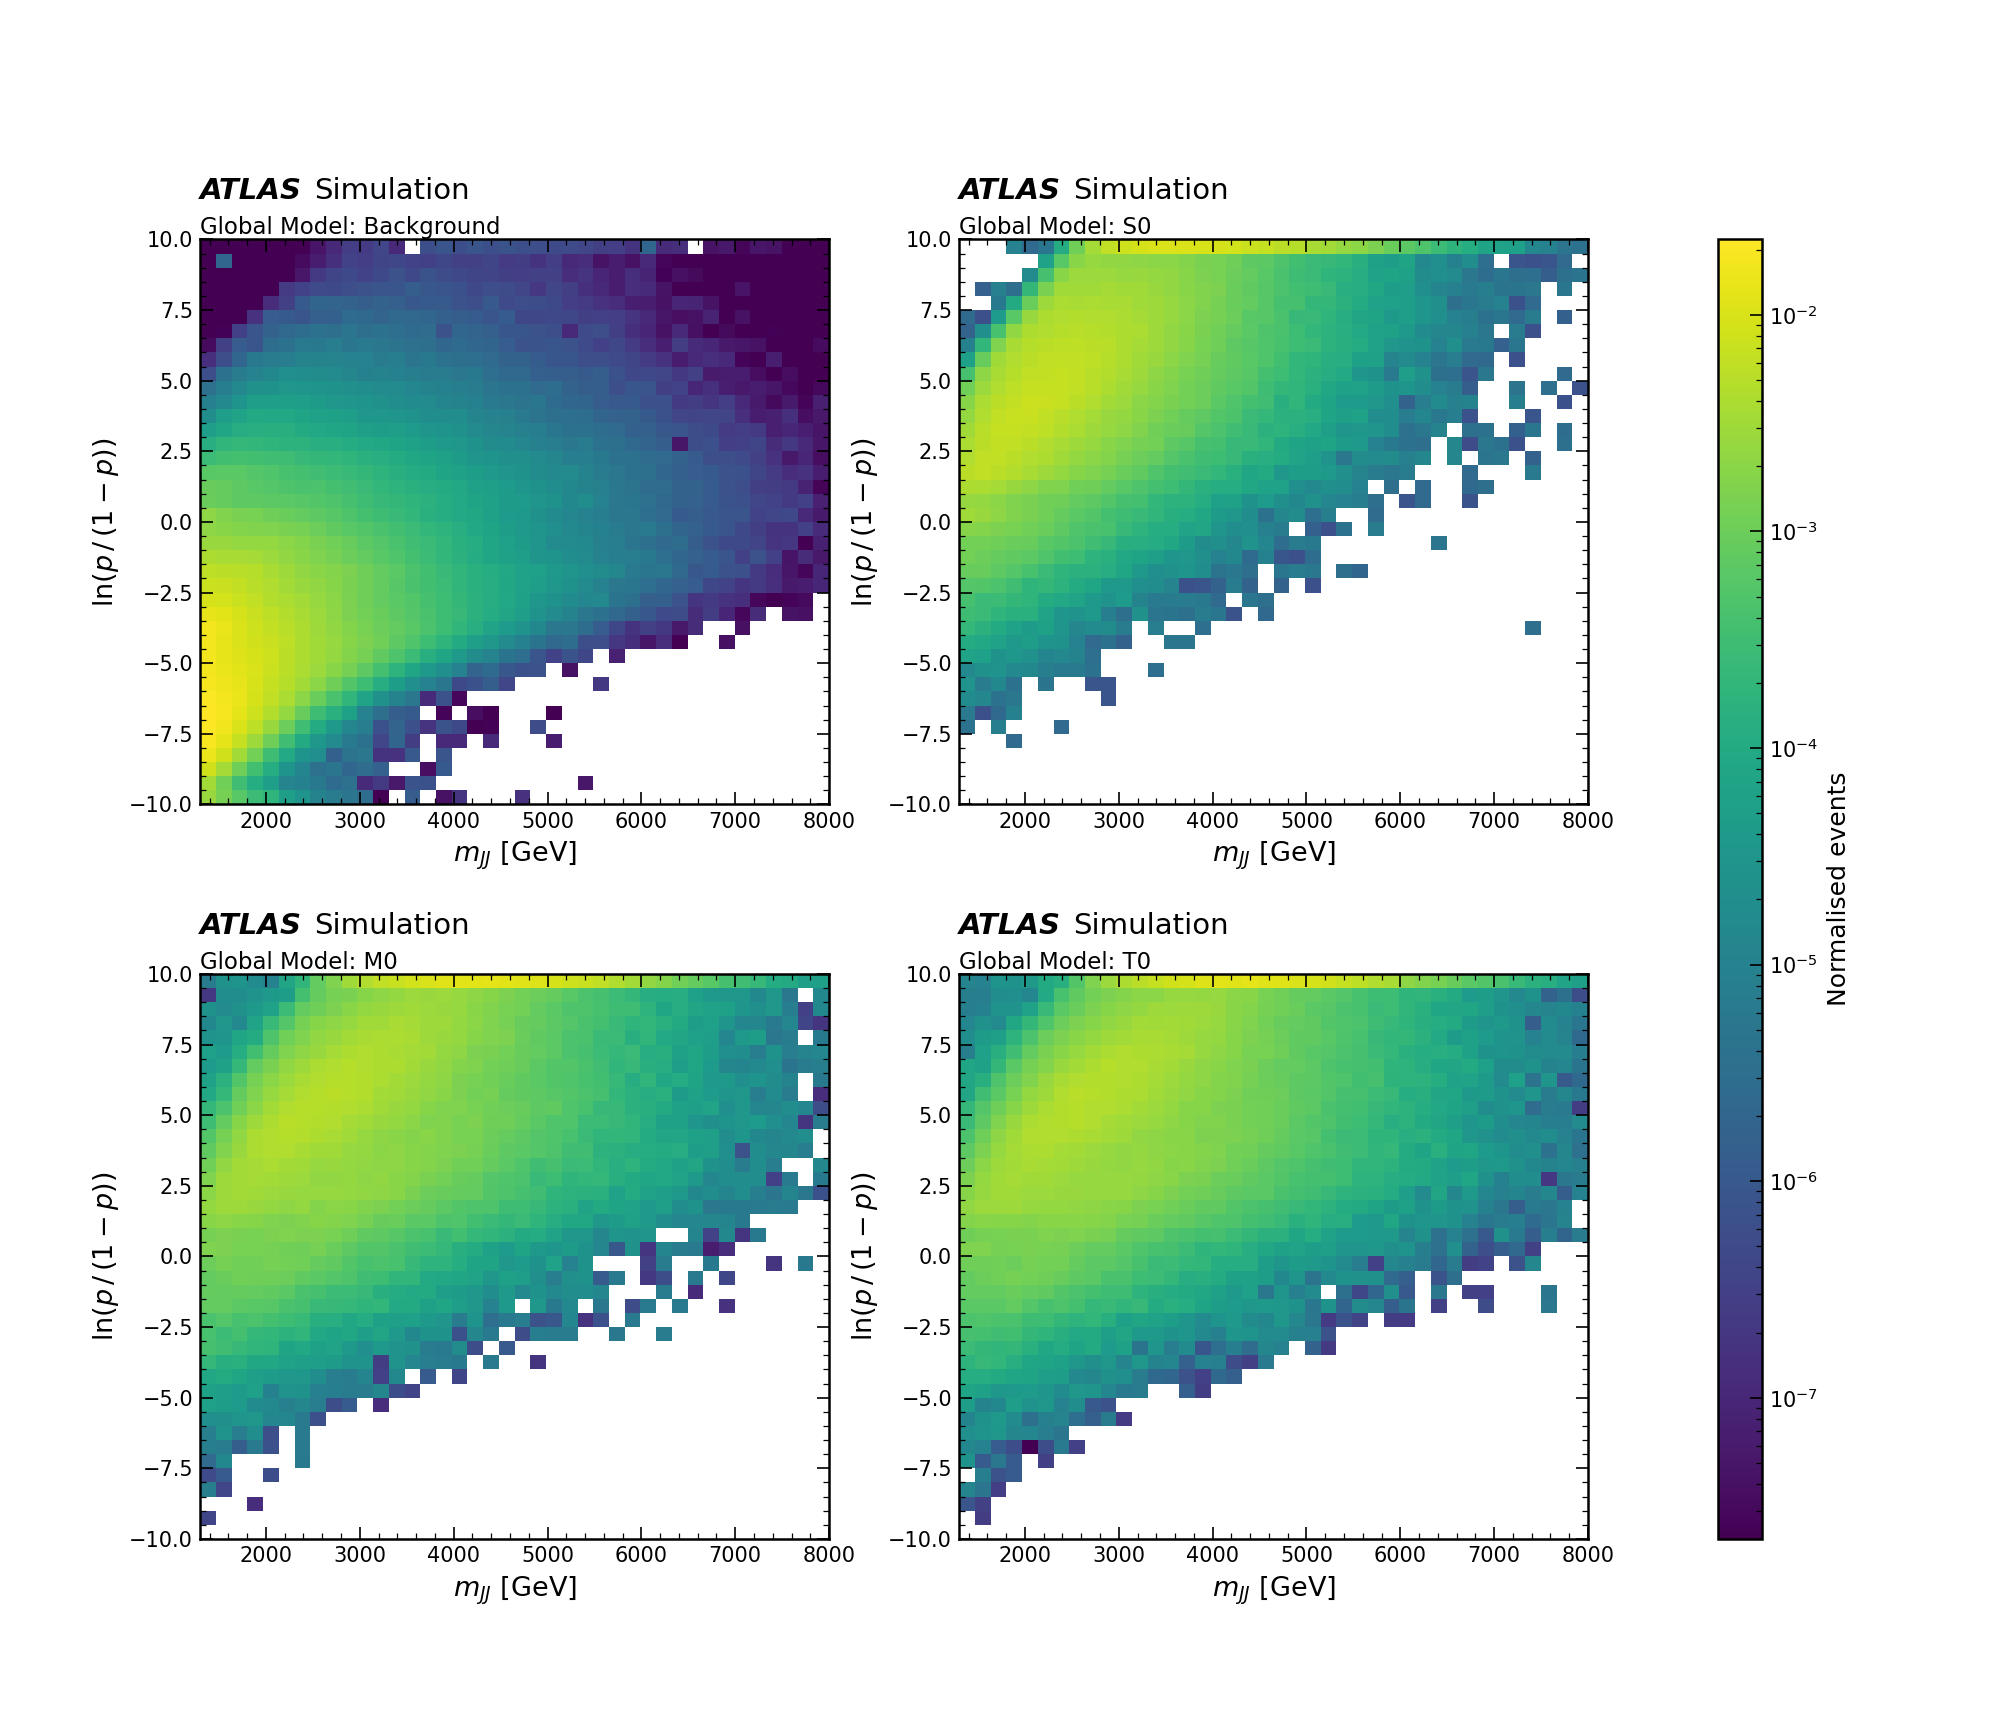
\includegraphics[width=\textwidth]{combined_var_disc-vbfrnn-v3-equal-signal-crosssection/binary_combined_JJ_M_NOSYS.png}
\caption{$m_{JJ}$.}
\end{subfigure}
\hfill
\begin{subfigure}[b]{0.38\textwidth}
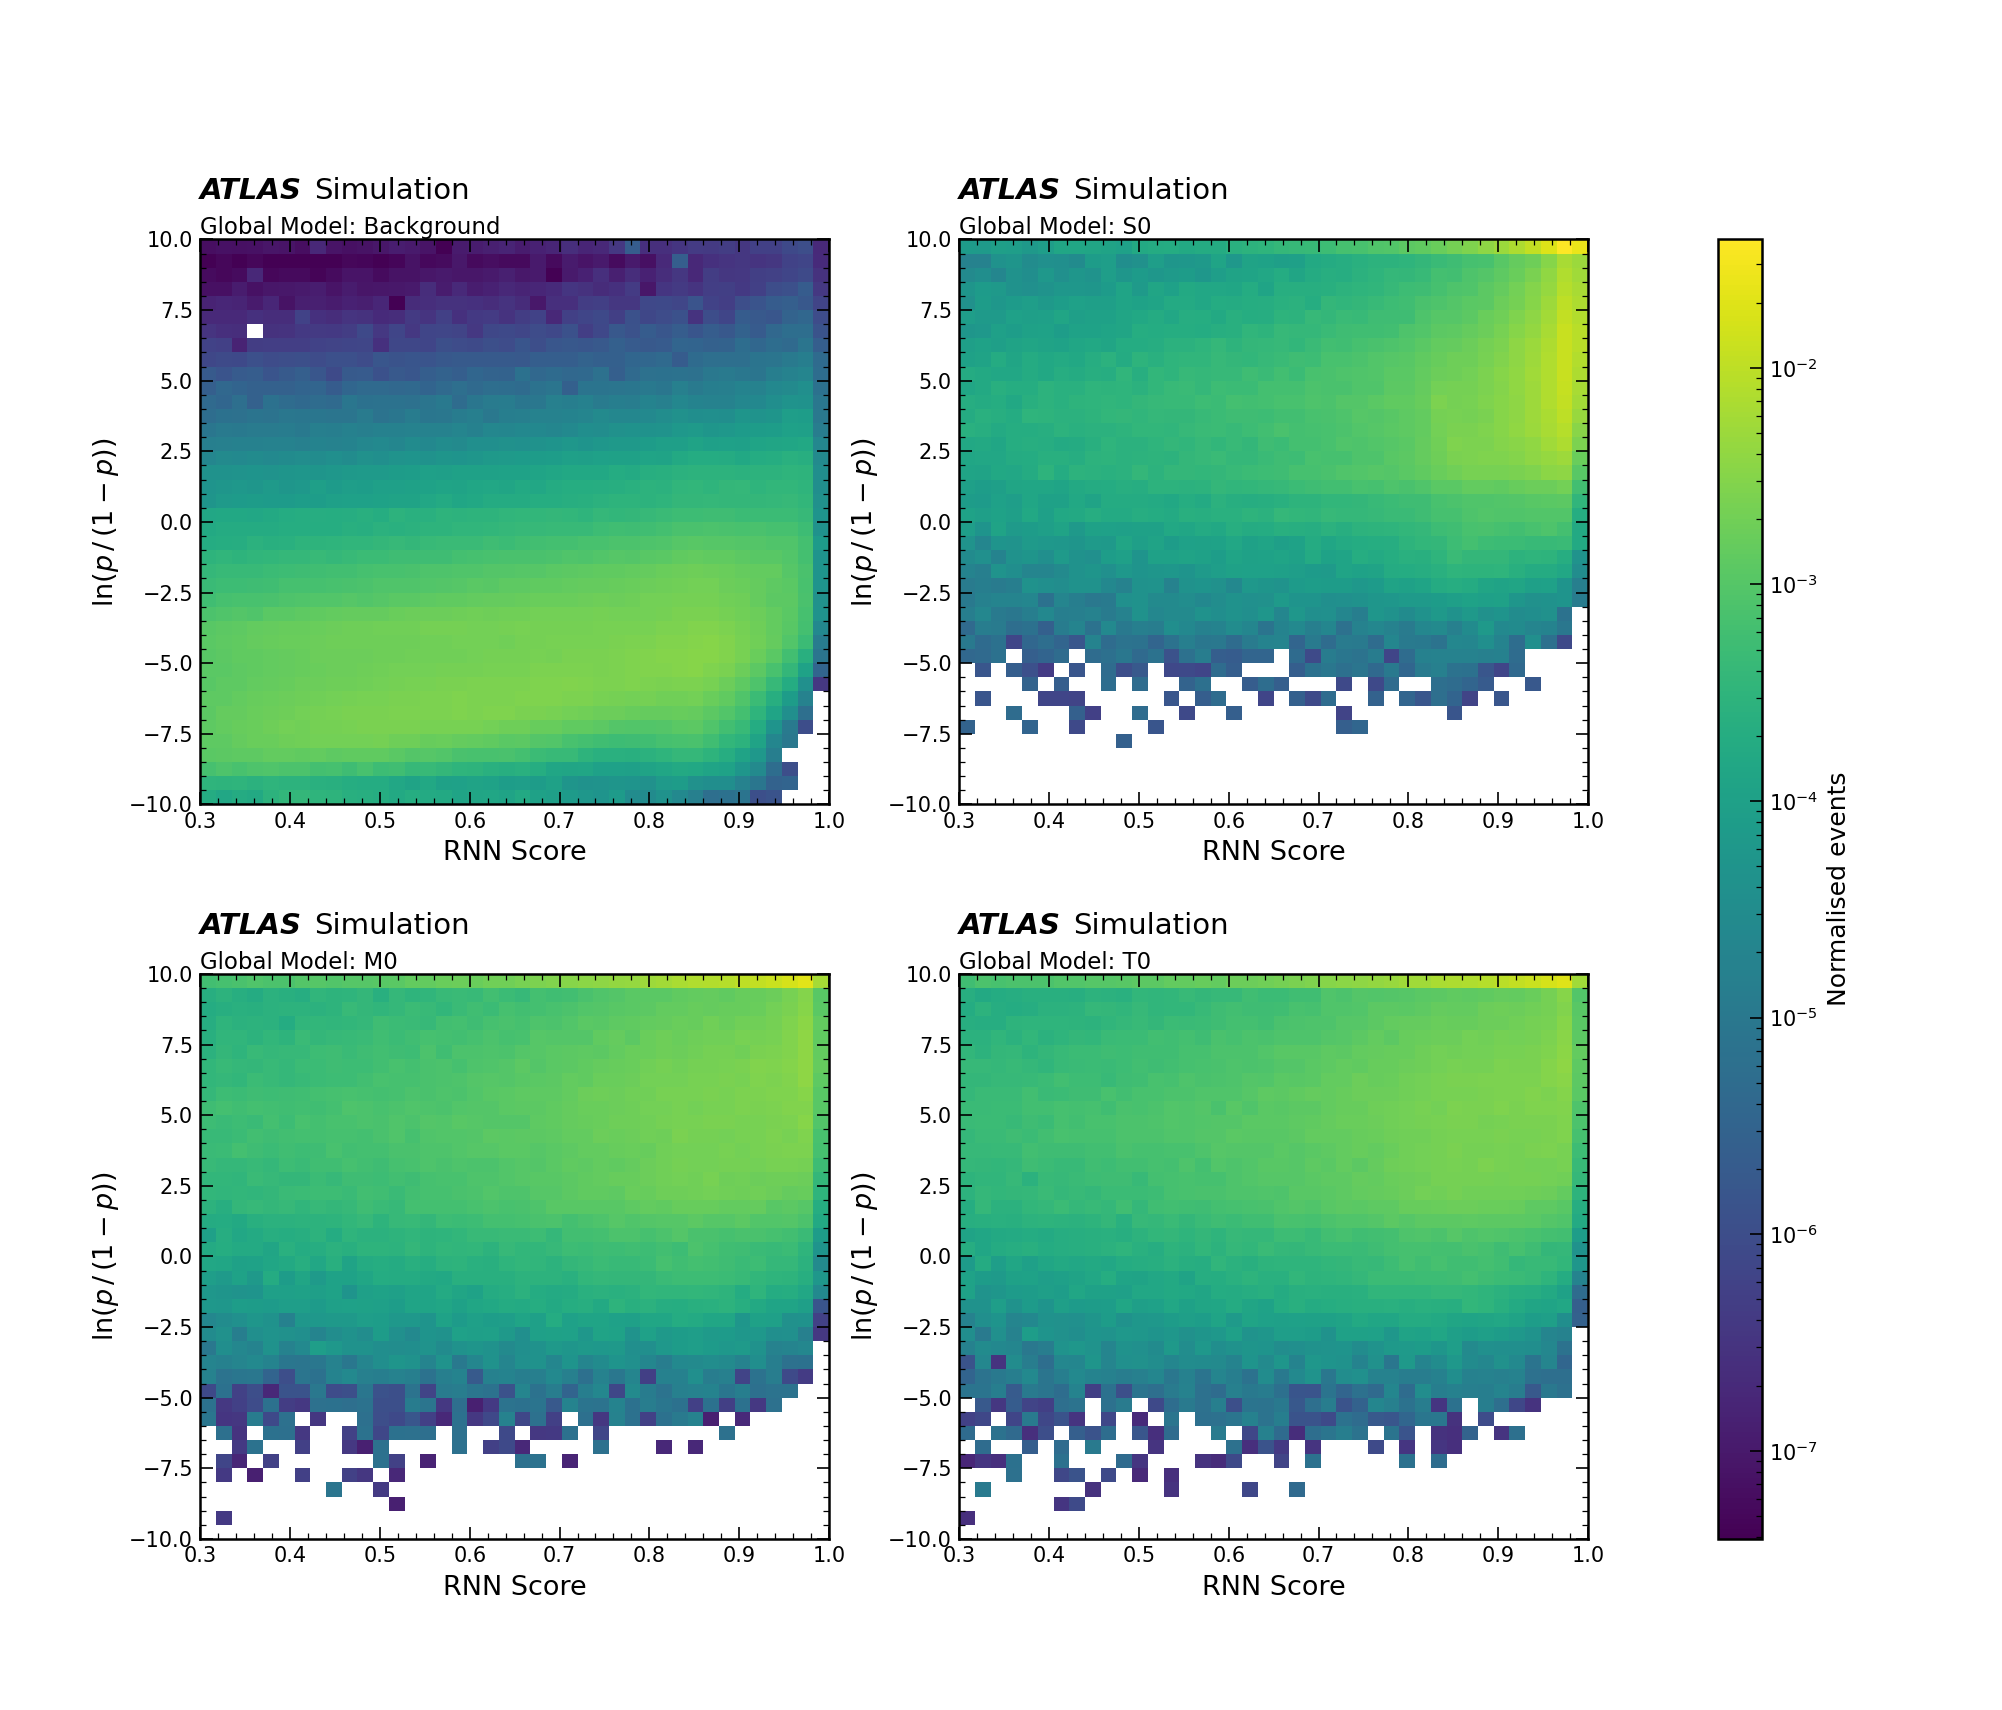
\includegraphics[width=\textwidth]{combined_var_disc-vbfrnn-v3-equal-signal-crosssection/binary_combined_RNNScore_NOSYS.png}
\caption{VBF-RNN score.}
\end{subfigure}

\medskip

\begin{subfigure}[b]{0.38\textwidth}
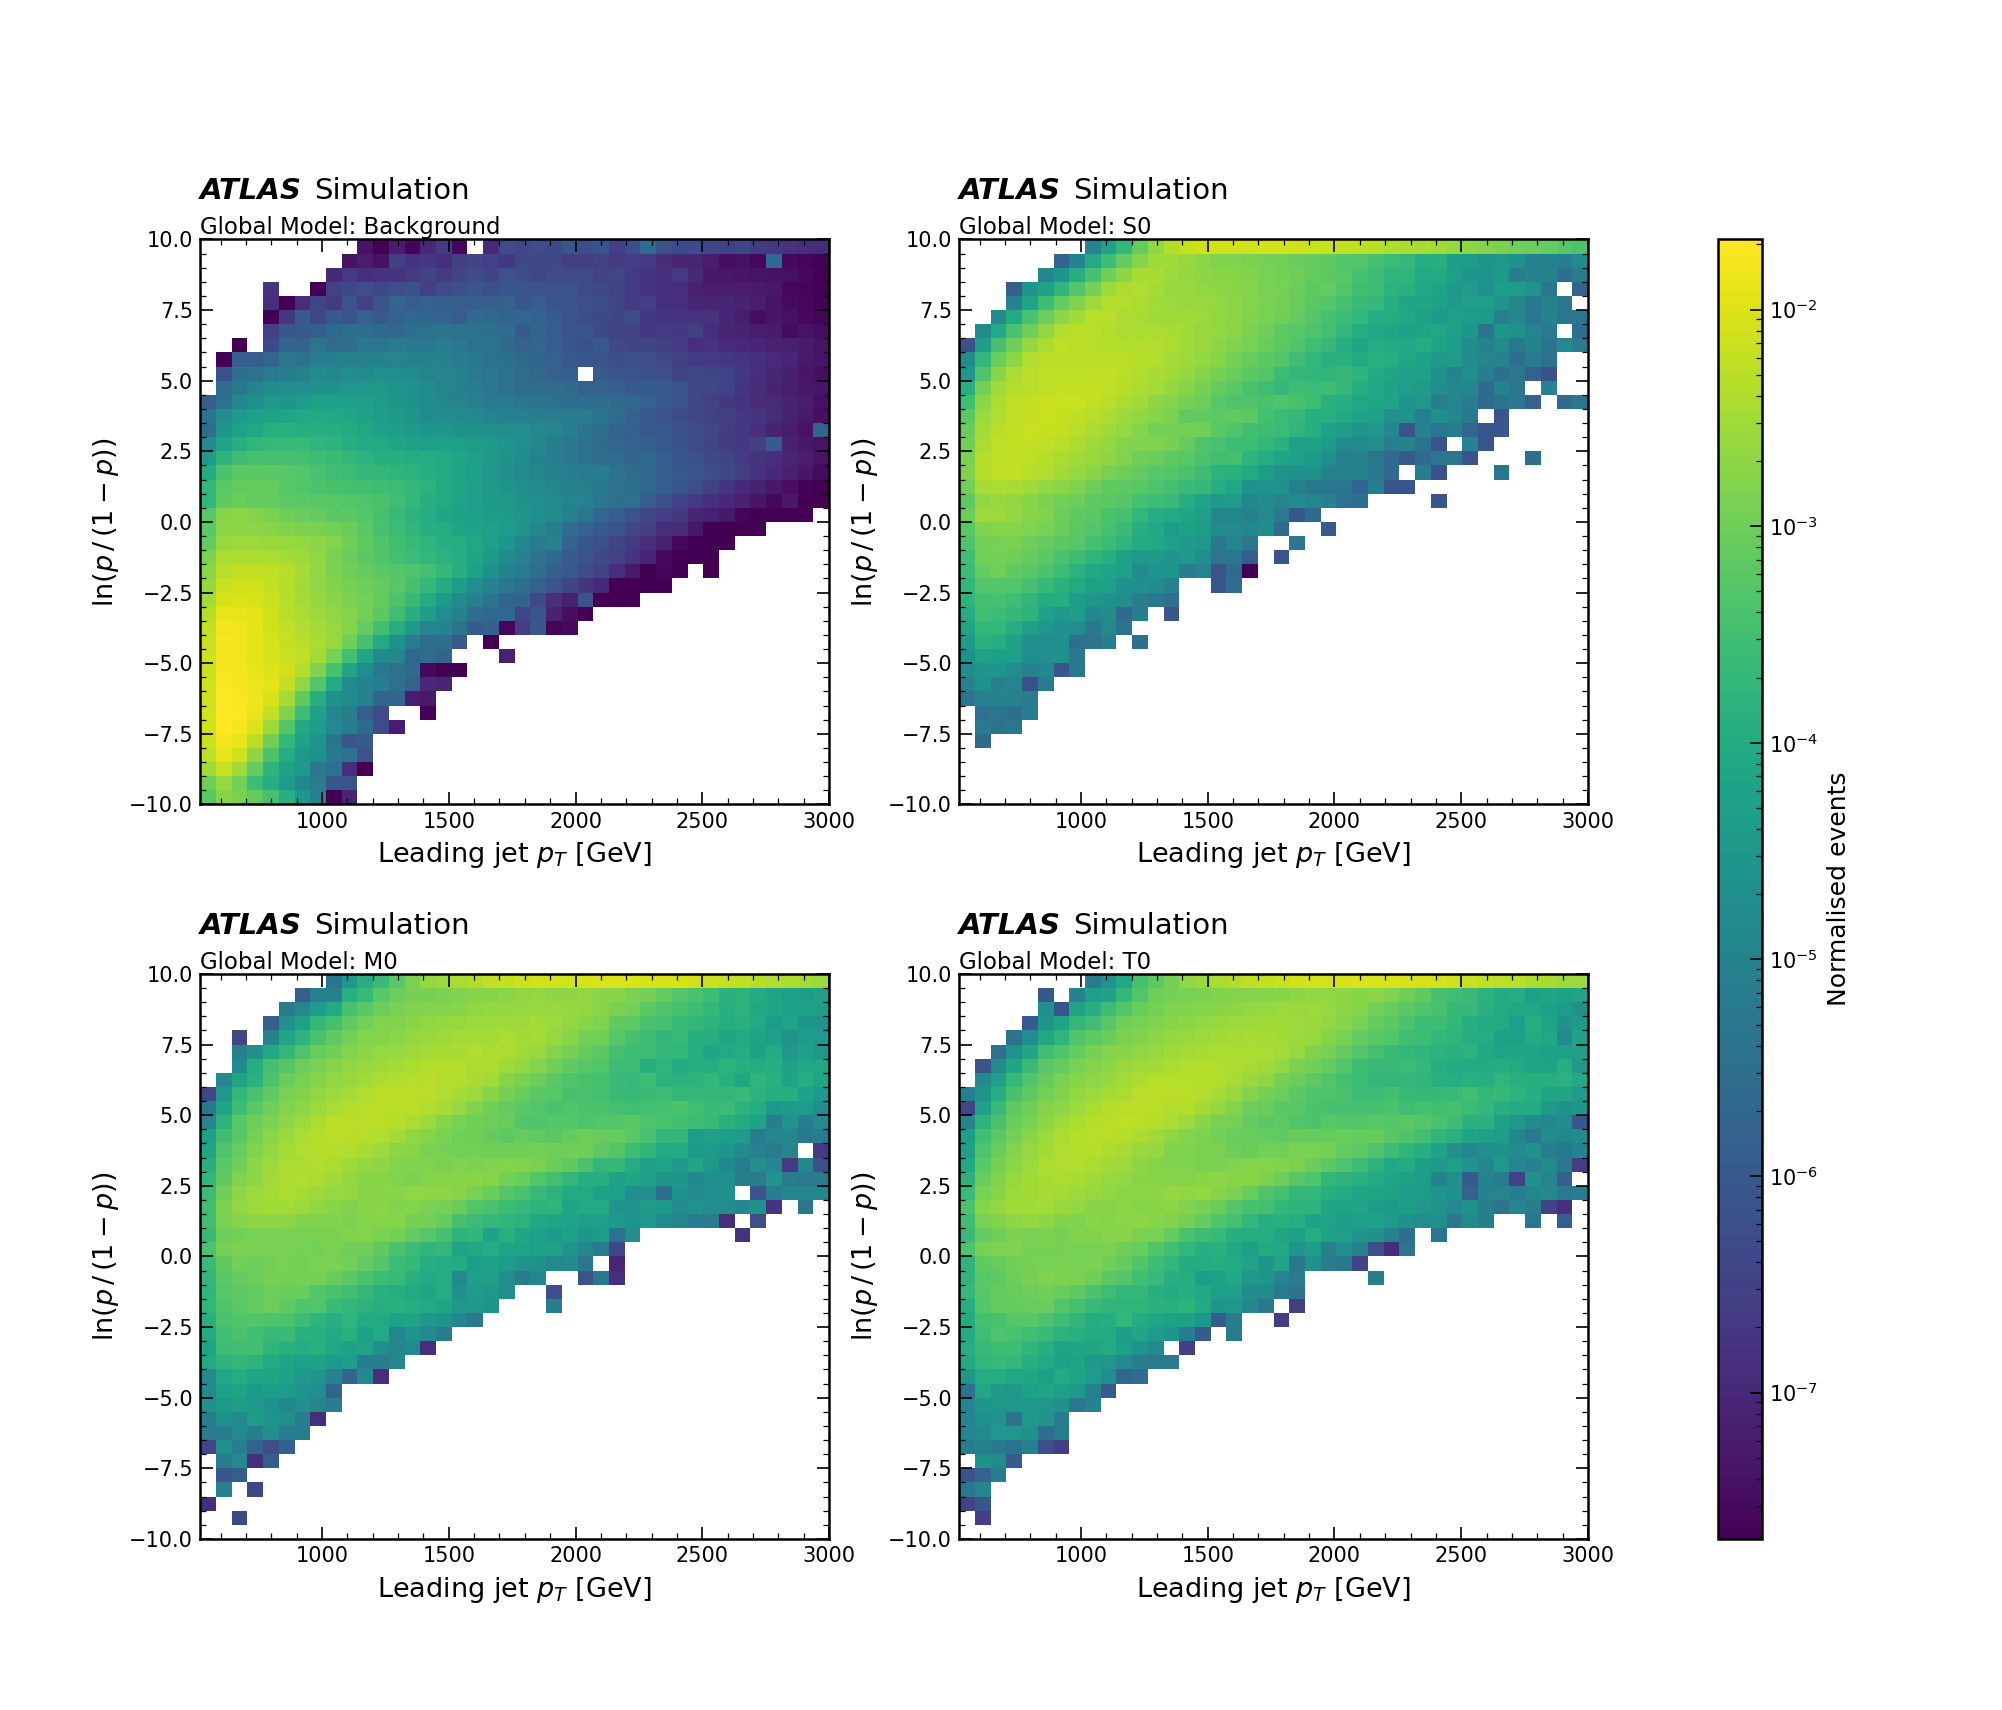
\includegraphics[width=\textwidth]{combined_var_disc-vbfrnn-v3-equal-signal-crosssection/binary_combined_SigJet1_pT_NOSYS.png}
\caption{Leading $p_T$.}
\end{subfigure}
\hfill
\begin{subfigure}[b]{0.38\textwidth}
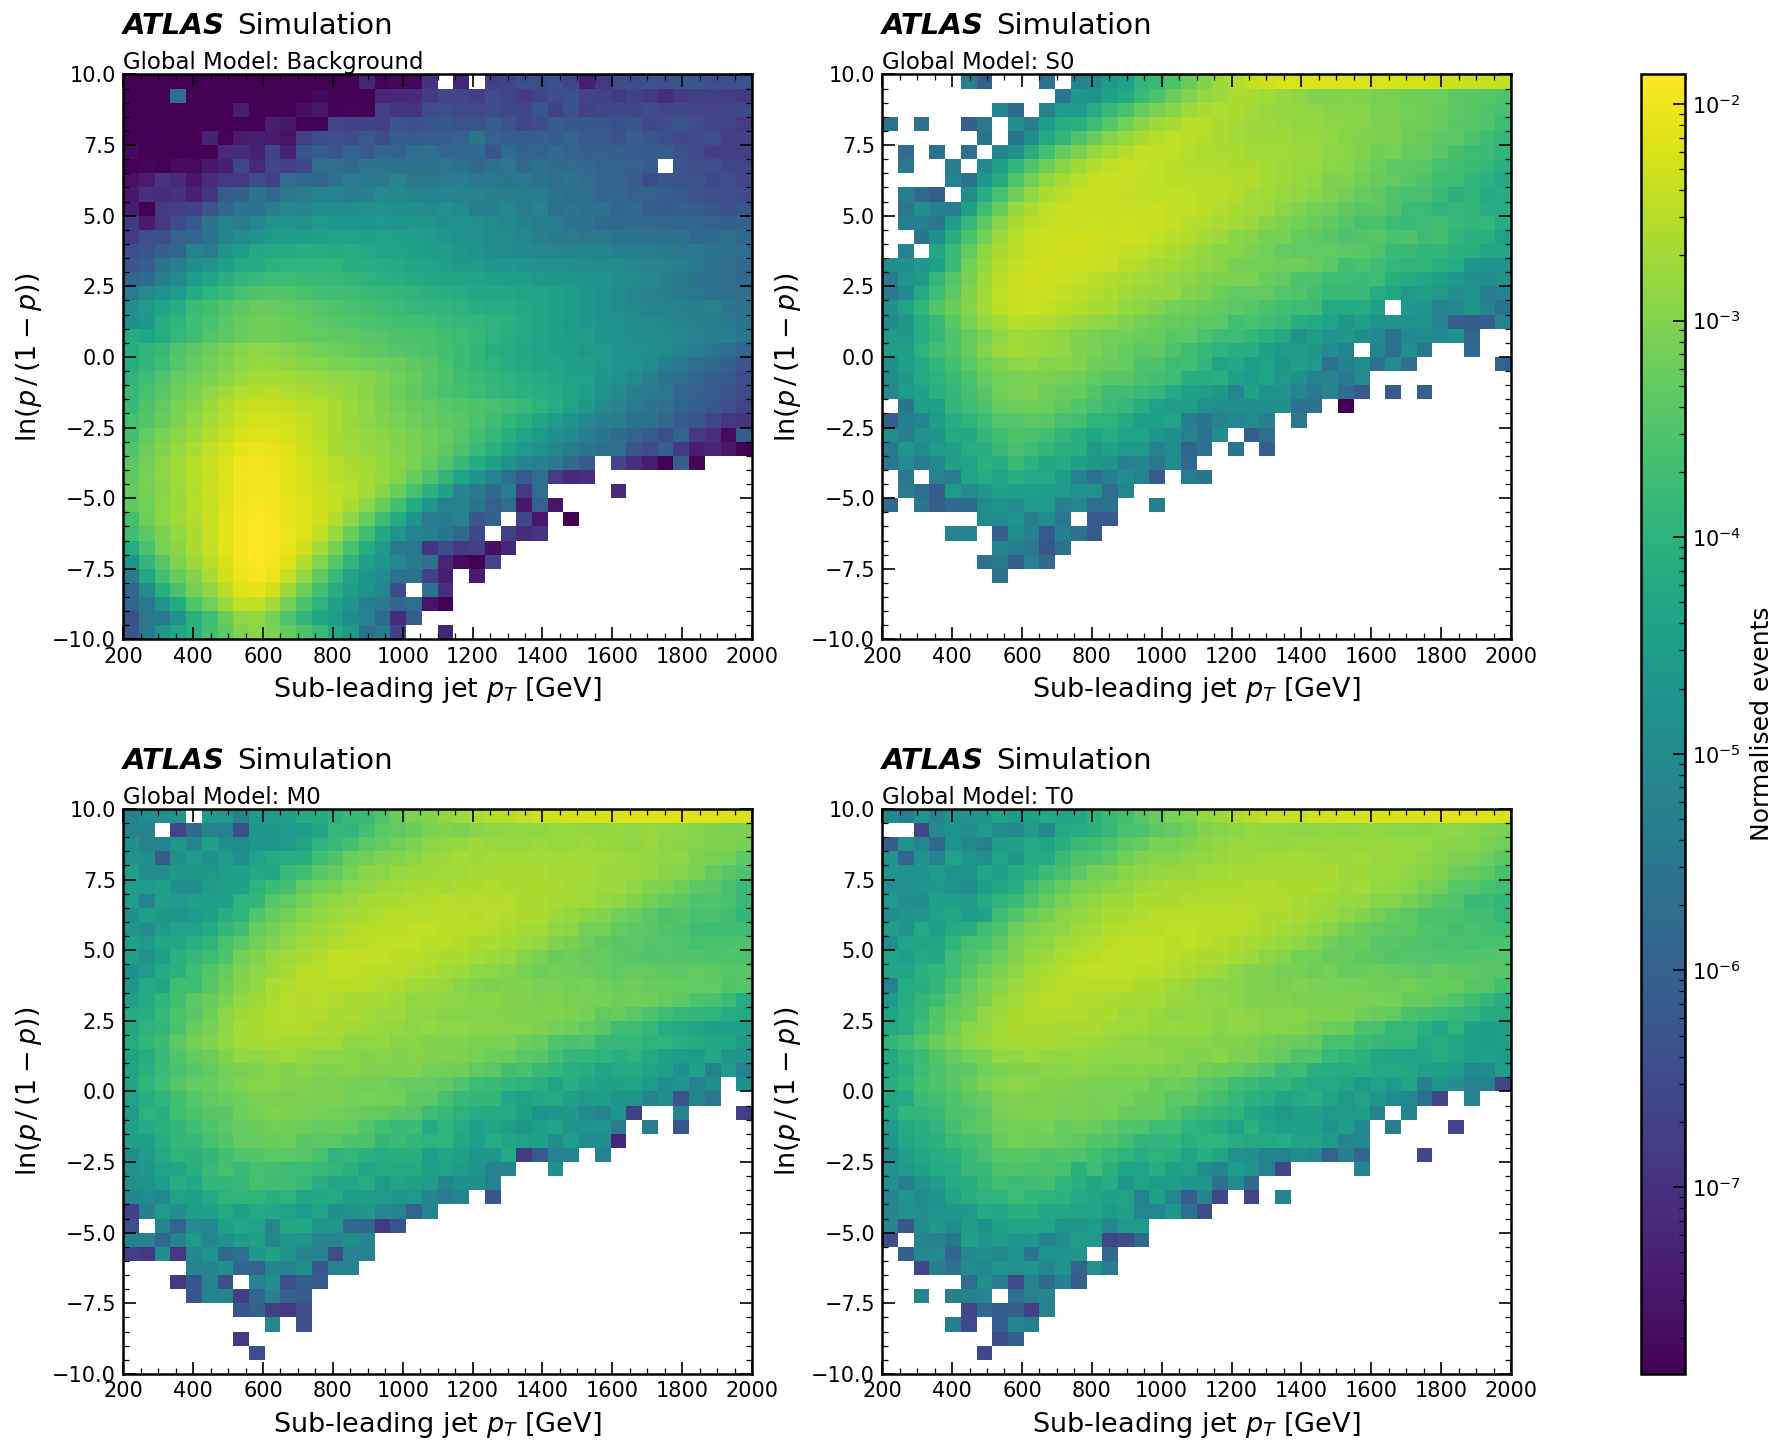
\includegraphics[width=\textwidth]{combined_var_disc-vbfrnn-v3-equal-signal-crosssection/binary_combined_SigJet2_pT_NOSYS.png}
\caption{Sub-leading $p_T$.}
\end{subfigure}

\medskip

\begin{subfigure}[b]{0.38\textwidth}
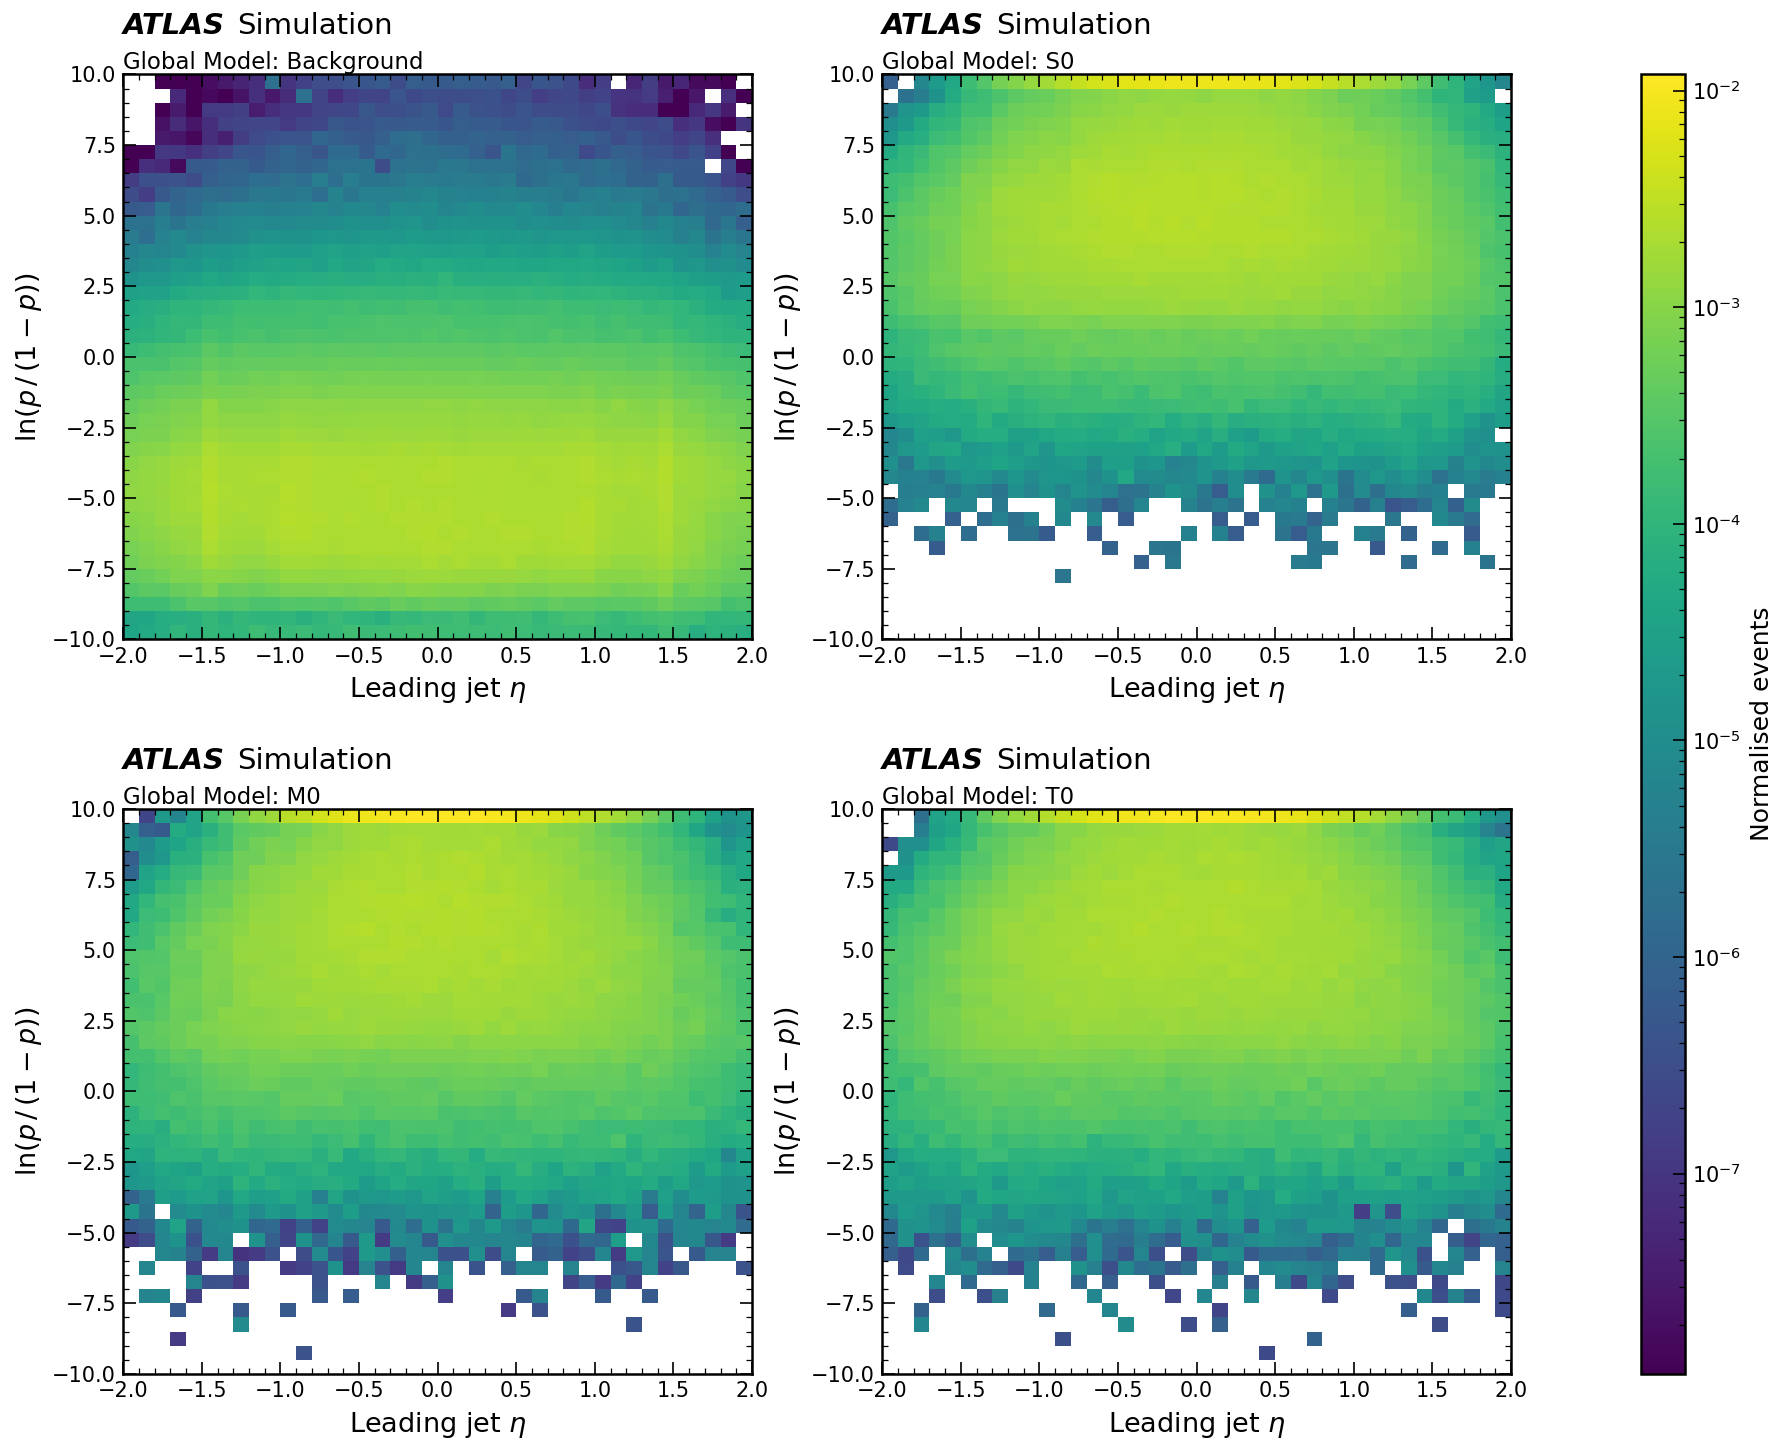
\includegraphics[width=\textwidth]{combined_var_disc-vbfrnn-v3-equal-signal-crosssection/binary_combined_SigJet1_eta_NOSYS.png}
\caption{Leading $\eta$.}
\end{subfigure}
\hfill
\begin{subfigure}[b]{0.38\textwidth}
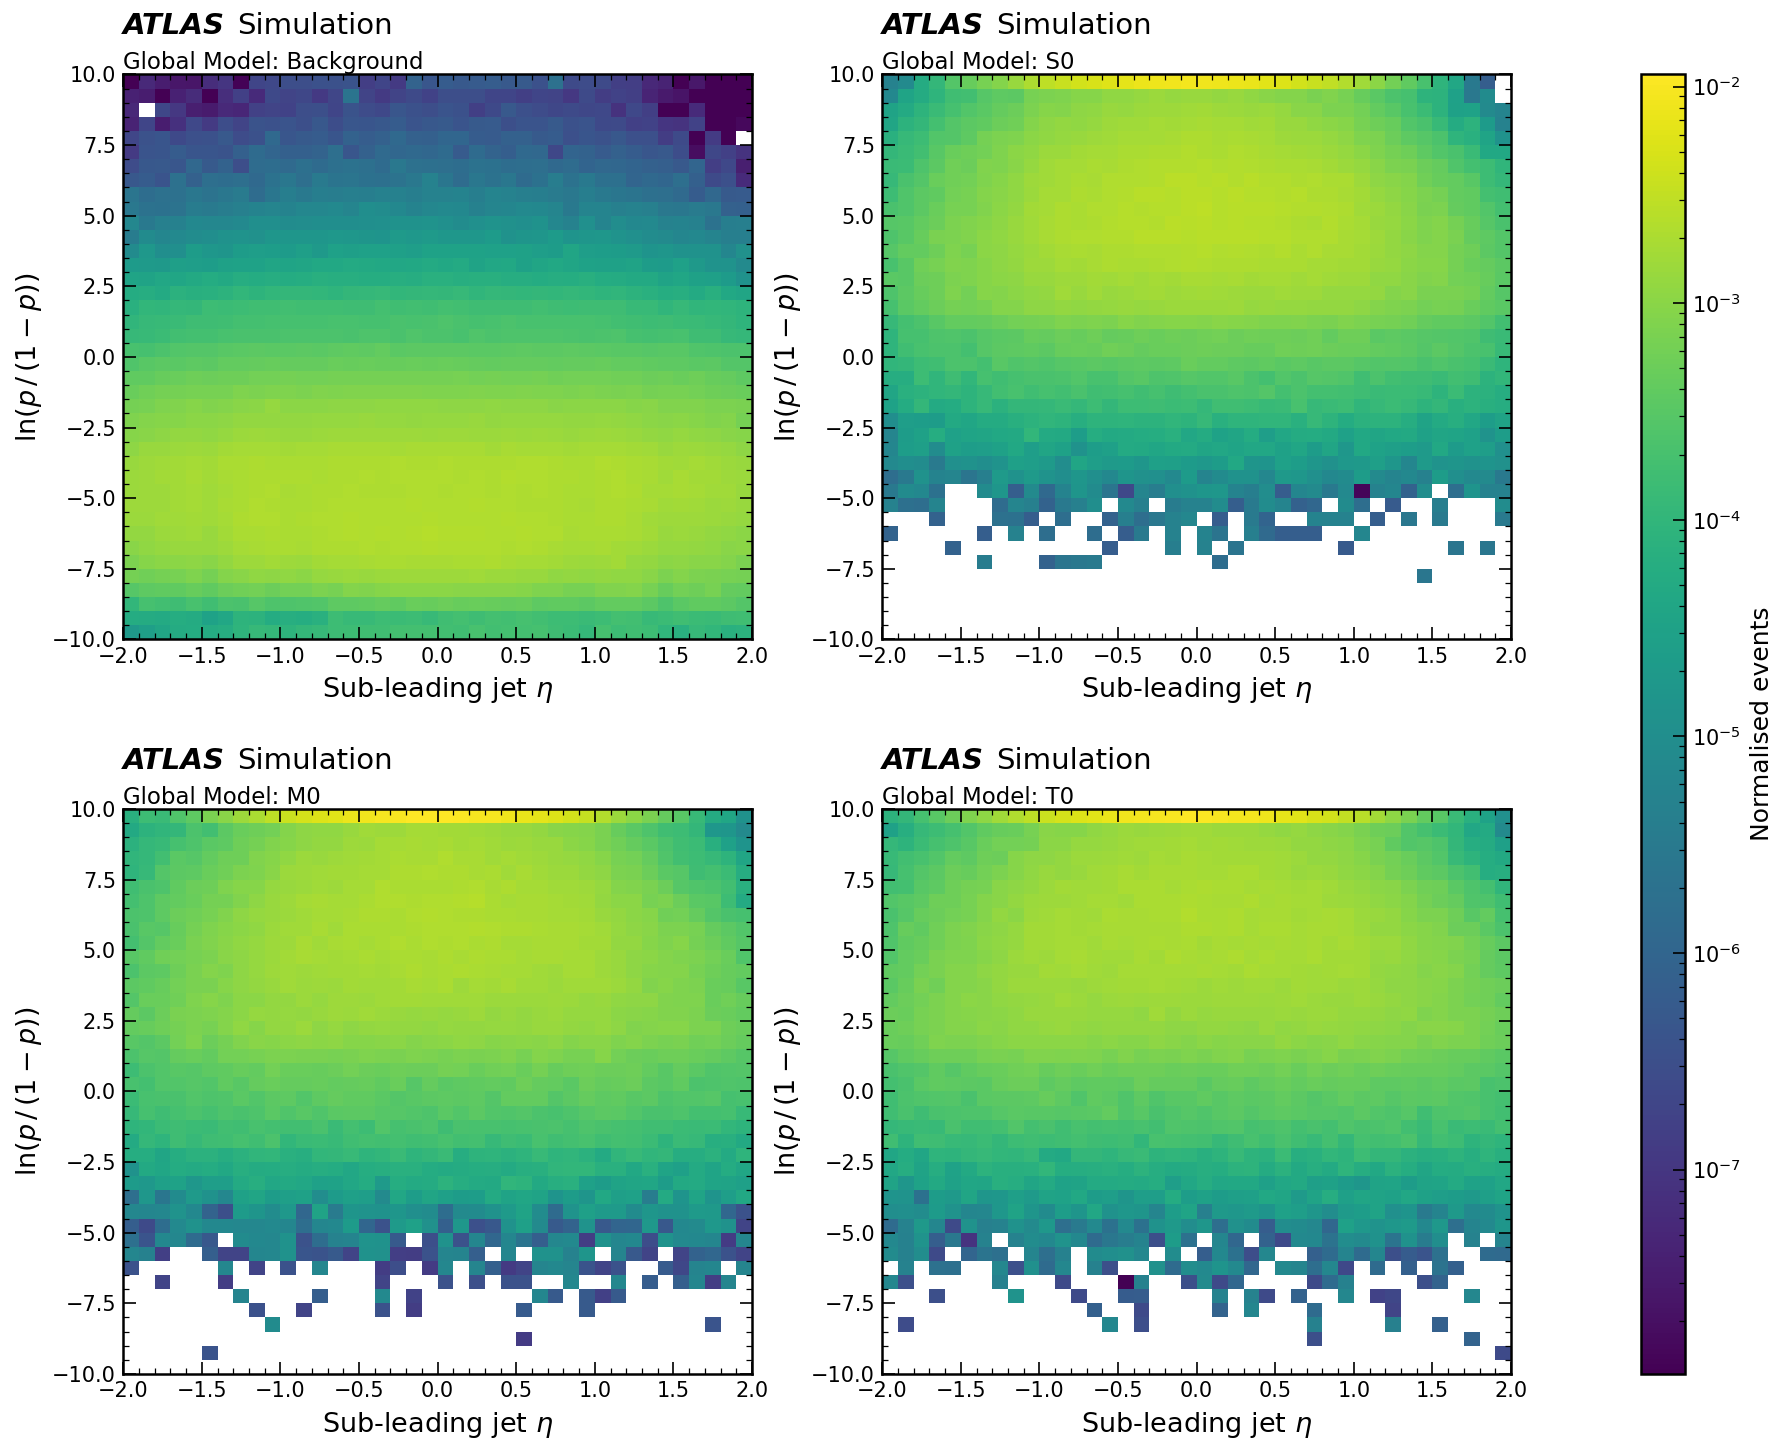
\includegraphics[width=\textwidth]{combined_var_disc-vbfrnn-v3-equal-signal-crosssection/binary_combined_SigJet2_eta_NOSYS.png}
\caption{Sub-leading $\eta$.}
\end{subfigure}
\caption{2D distribution of the global binary discriminant using the v3~+~equal-$\sigma$ version.}
\label{fig:app_corr_binary}
\end{figure}

\begin{figure}[htbp]
\centering
\begin{subfigure}[b]{0.38\textwidth}
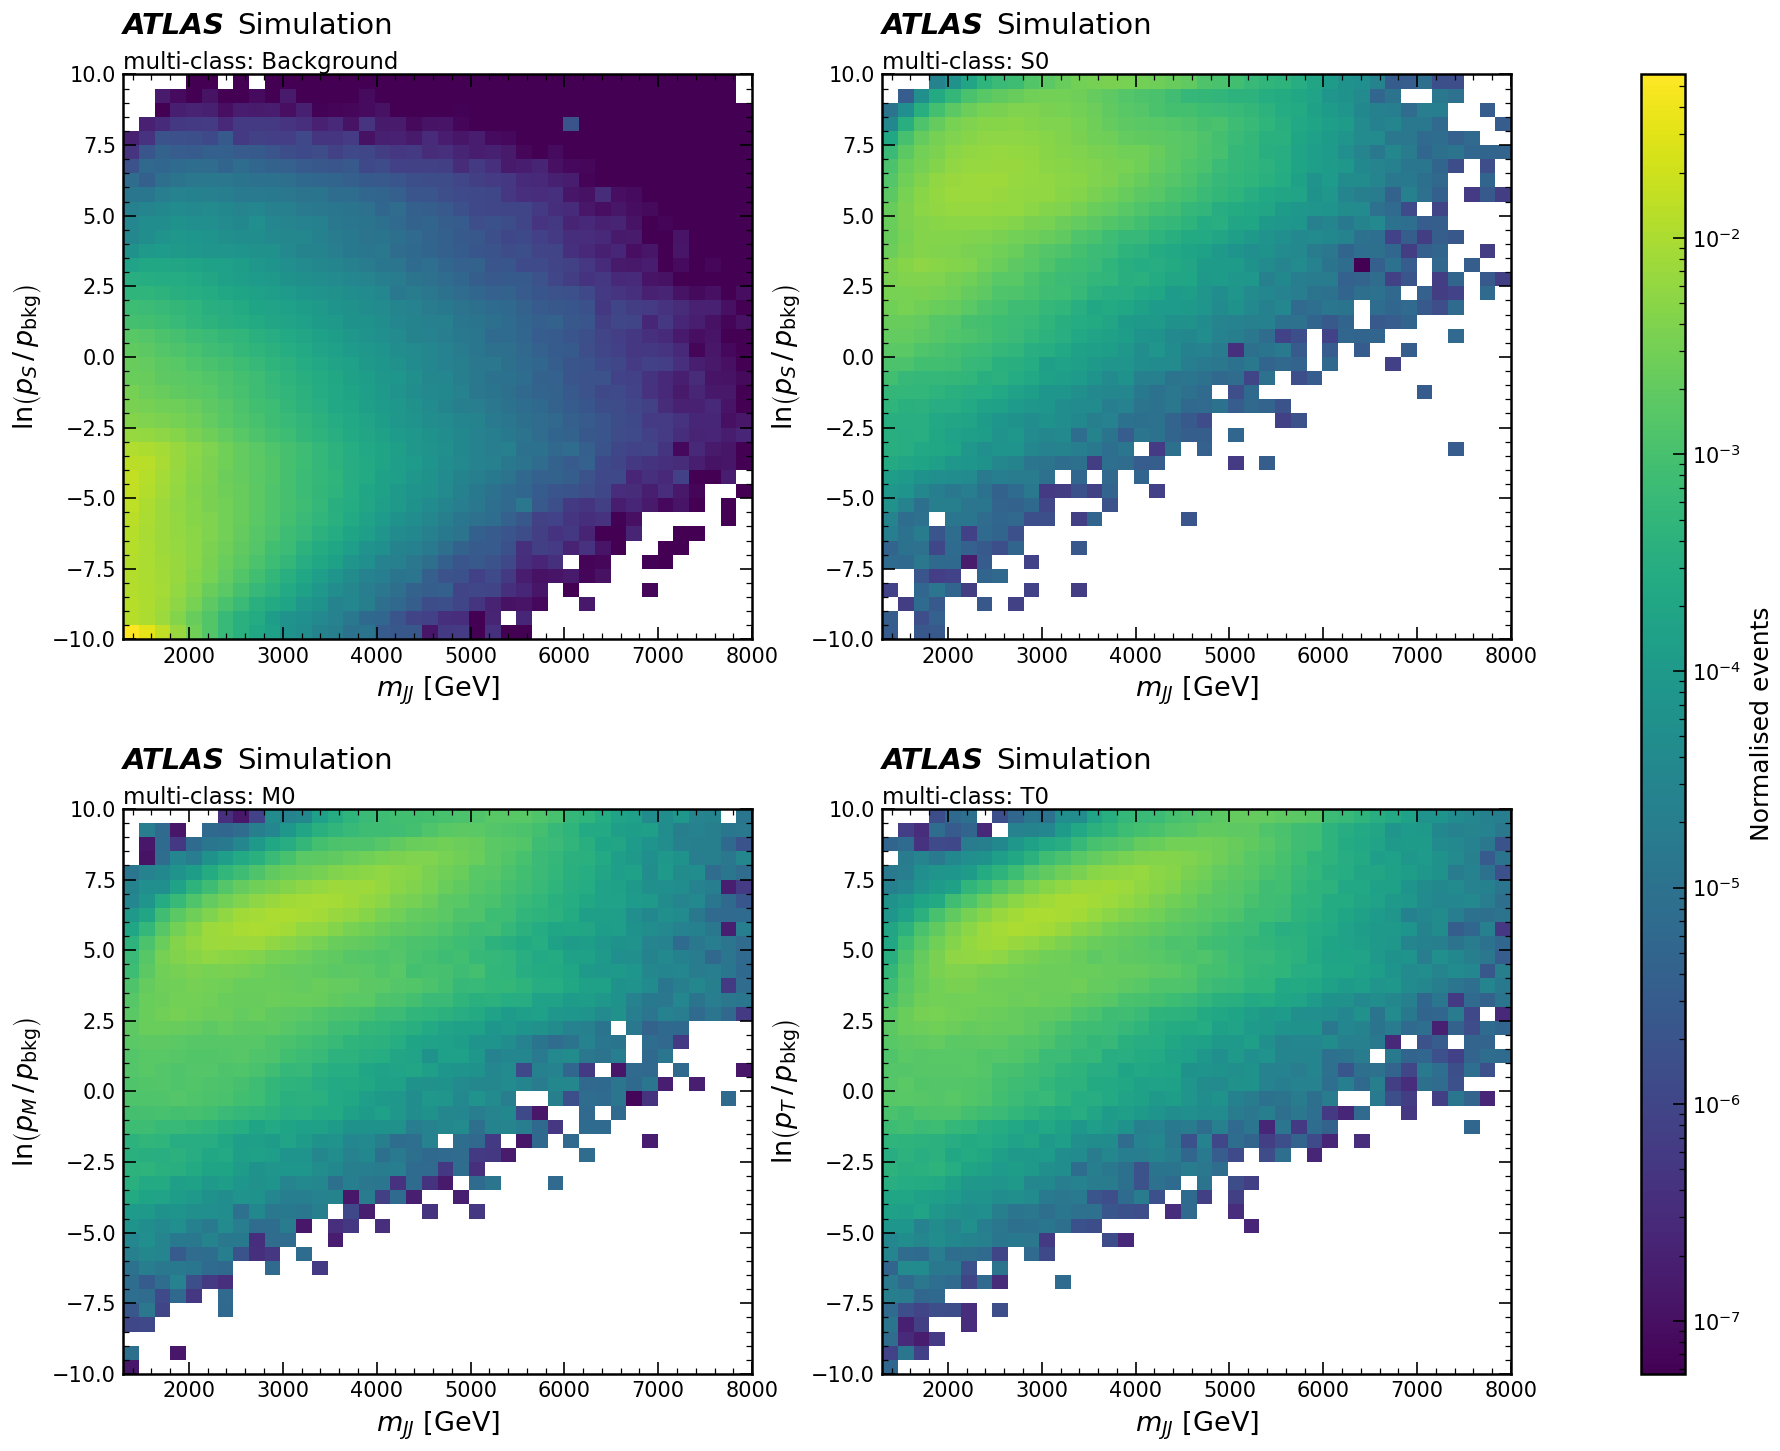
\includegraphics[width=\textwidth]{combined_var_disc-vbfrnn-v3-equal-signal-crosssection/mc01_combined_JJ_M_NOSYS.png}
\caption{$m_{JJ}$.}
\end{subfigure}
\hfill
\begin{subfigure}[b]{0.38\textwidth}
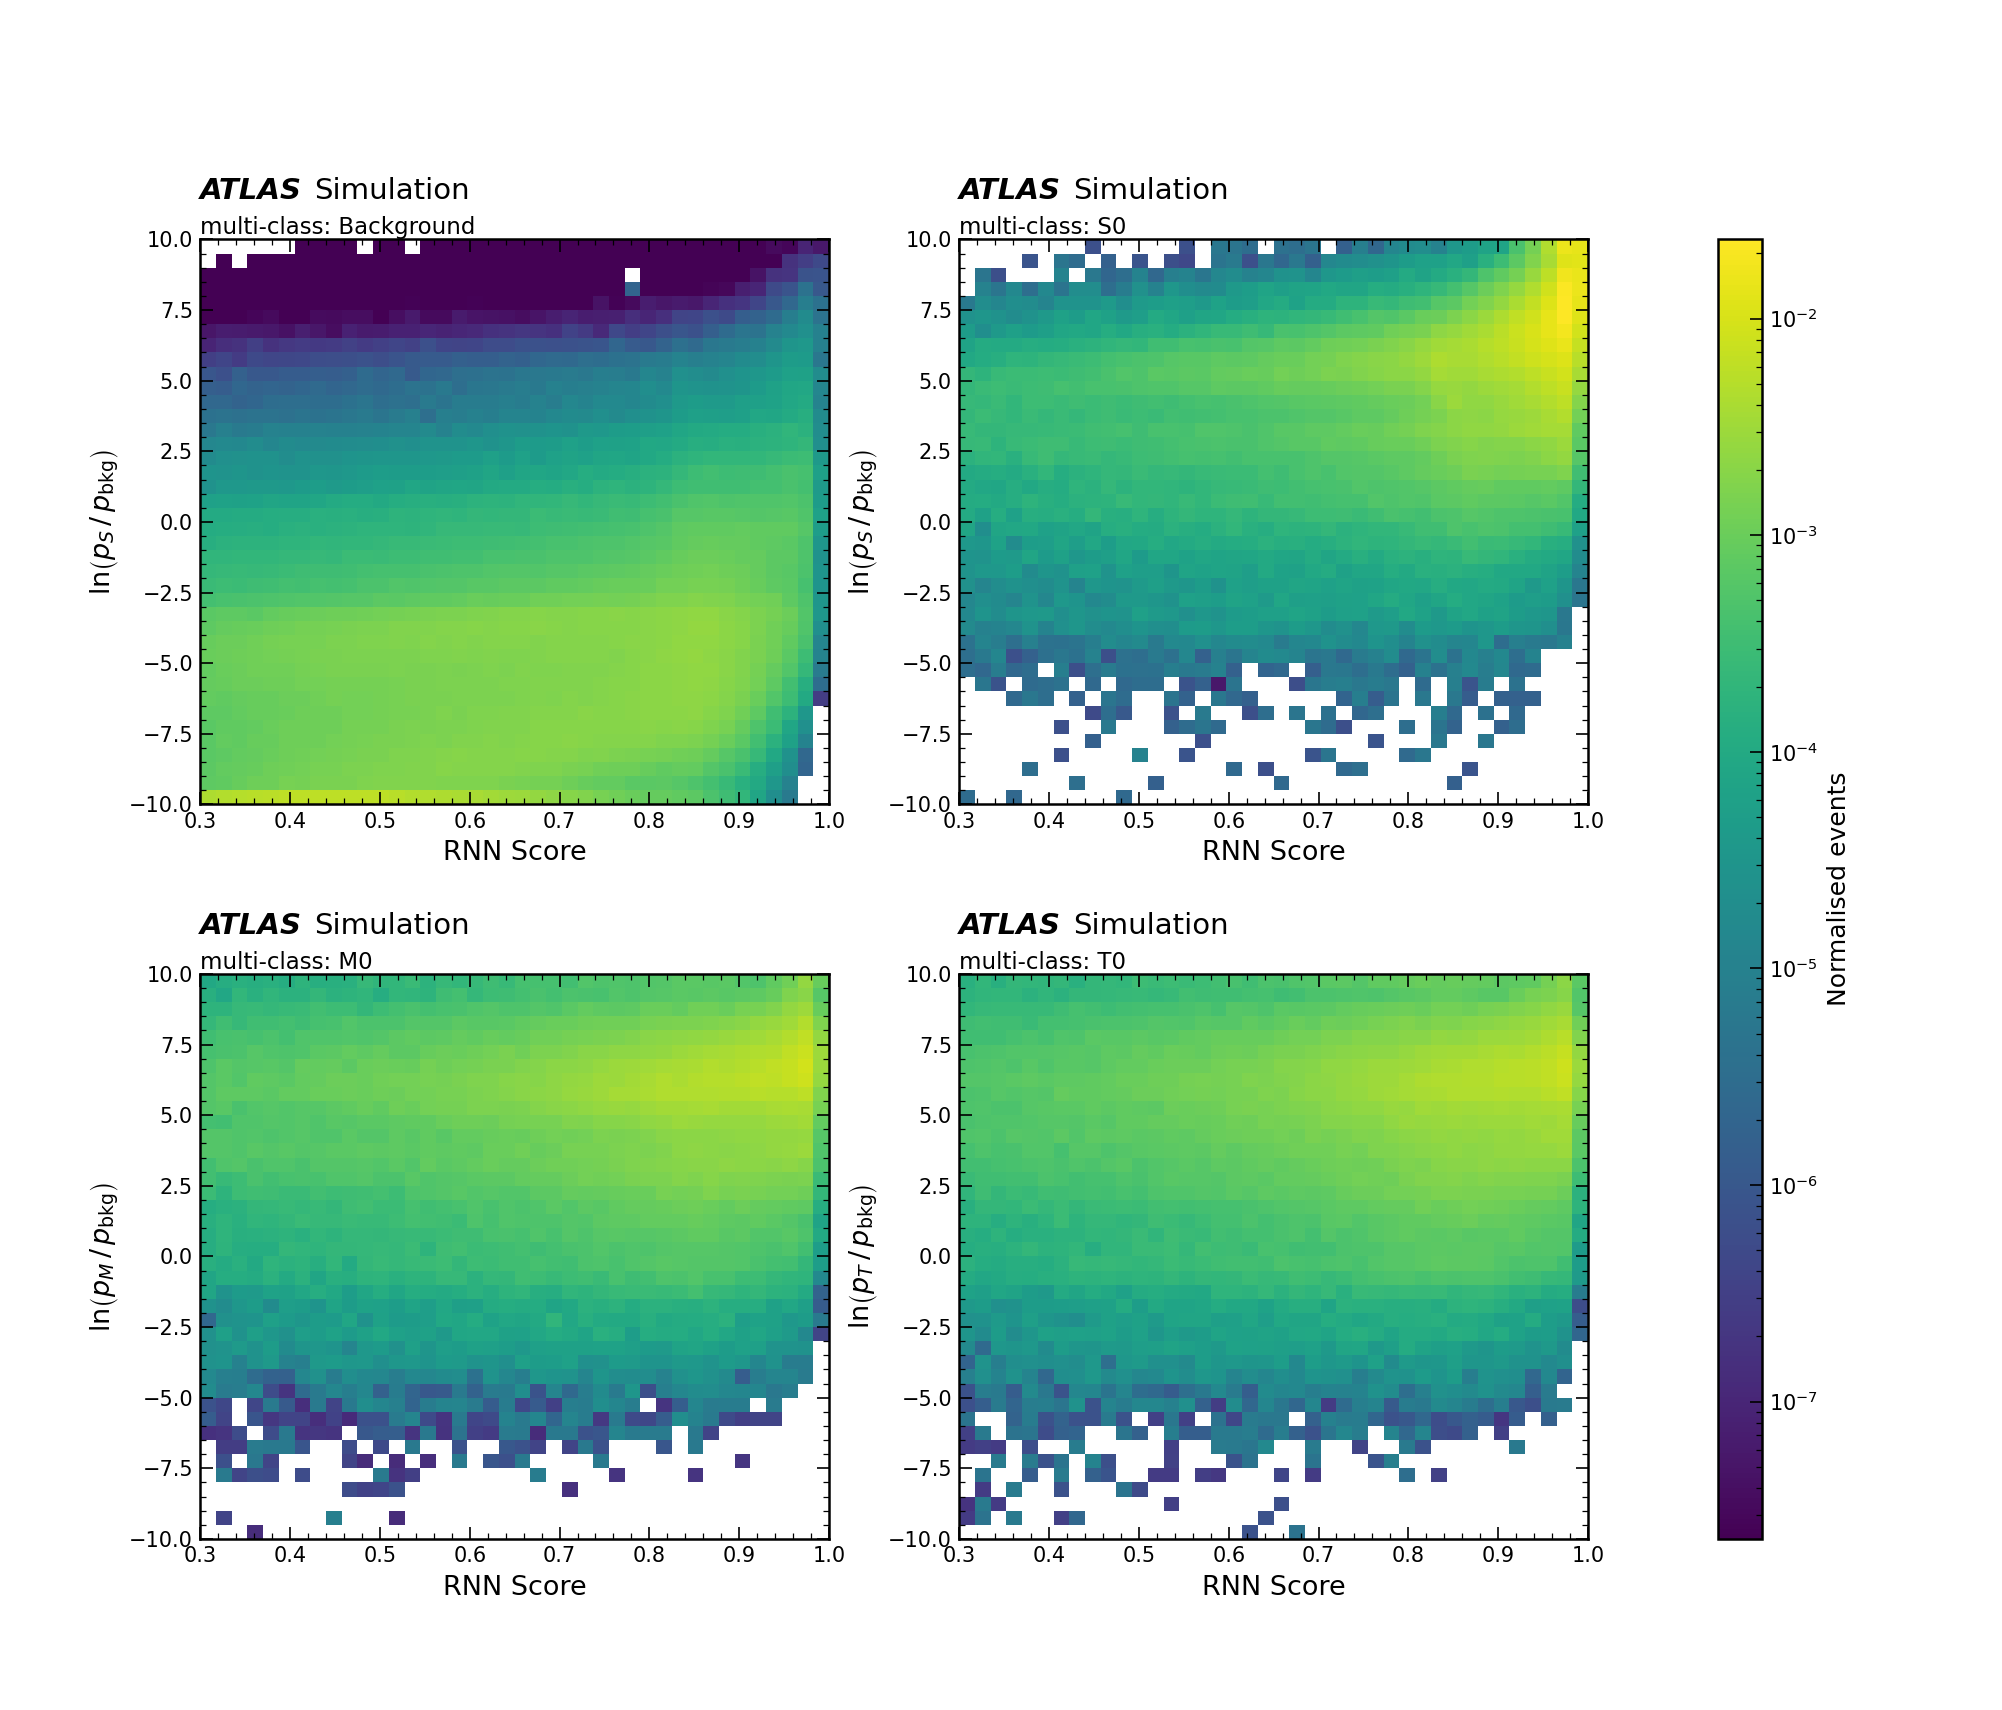
\includegraphics[width=\textwidth]{combined_var_disc-vbfrnn-v3-equal-signal-crosssection/mc01_combined_RNNScore_NOSYS.png}
\caption{VBF-RNN score.}
\end{subfigure}

\medskip

\begin{subfigure}[b]{0.38\textwidth}
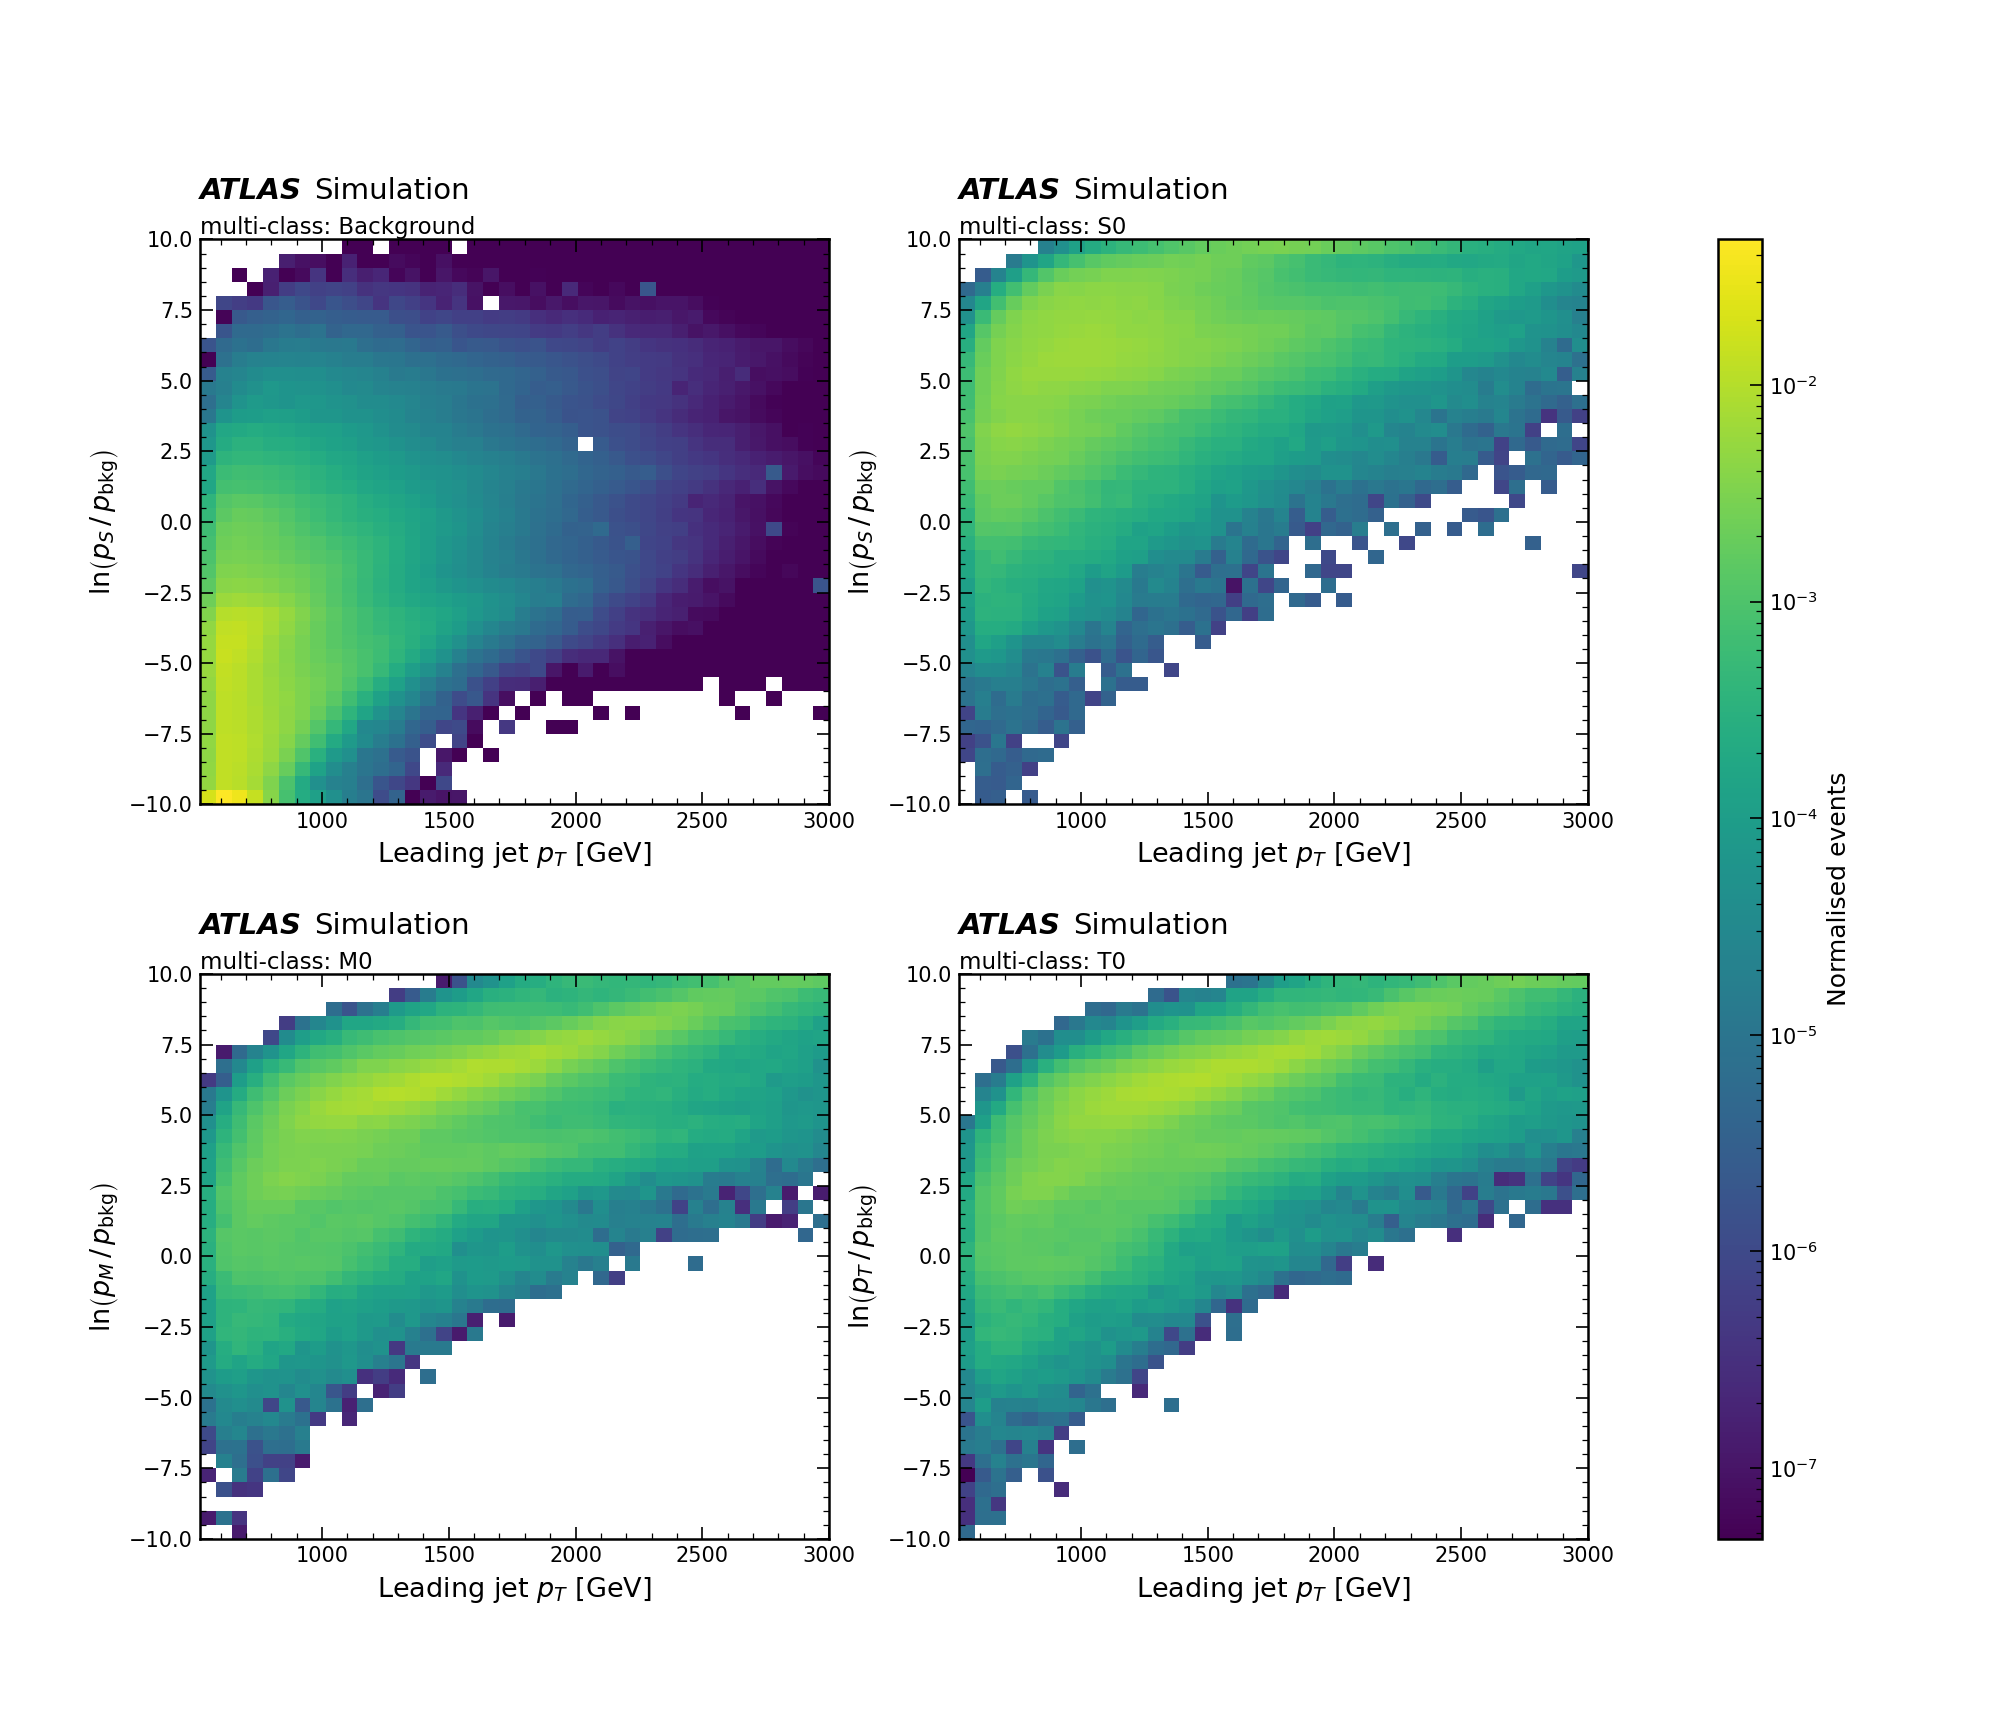
\includegraphics[width=\textwidth]{combined_var_disc-vbfrnn-v3-equal-signal-crosssection/mc01_combined_SigJet1_pT_NOSYS.png}
\caption{Leading $p_T$.}
\end{subfigure}
\hfill
\begin{subfigure}[b]{0.38\textwidth}
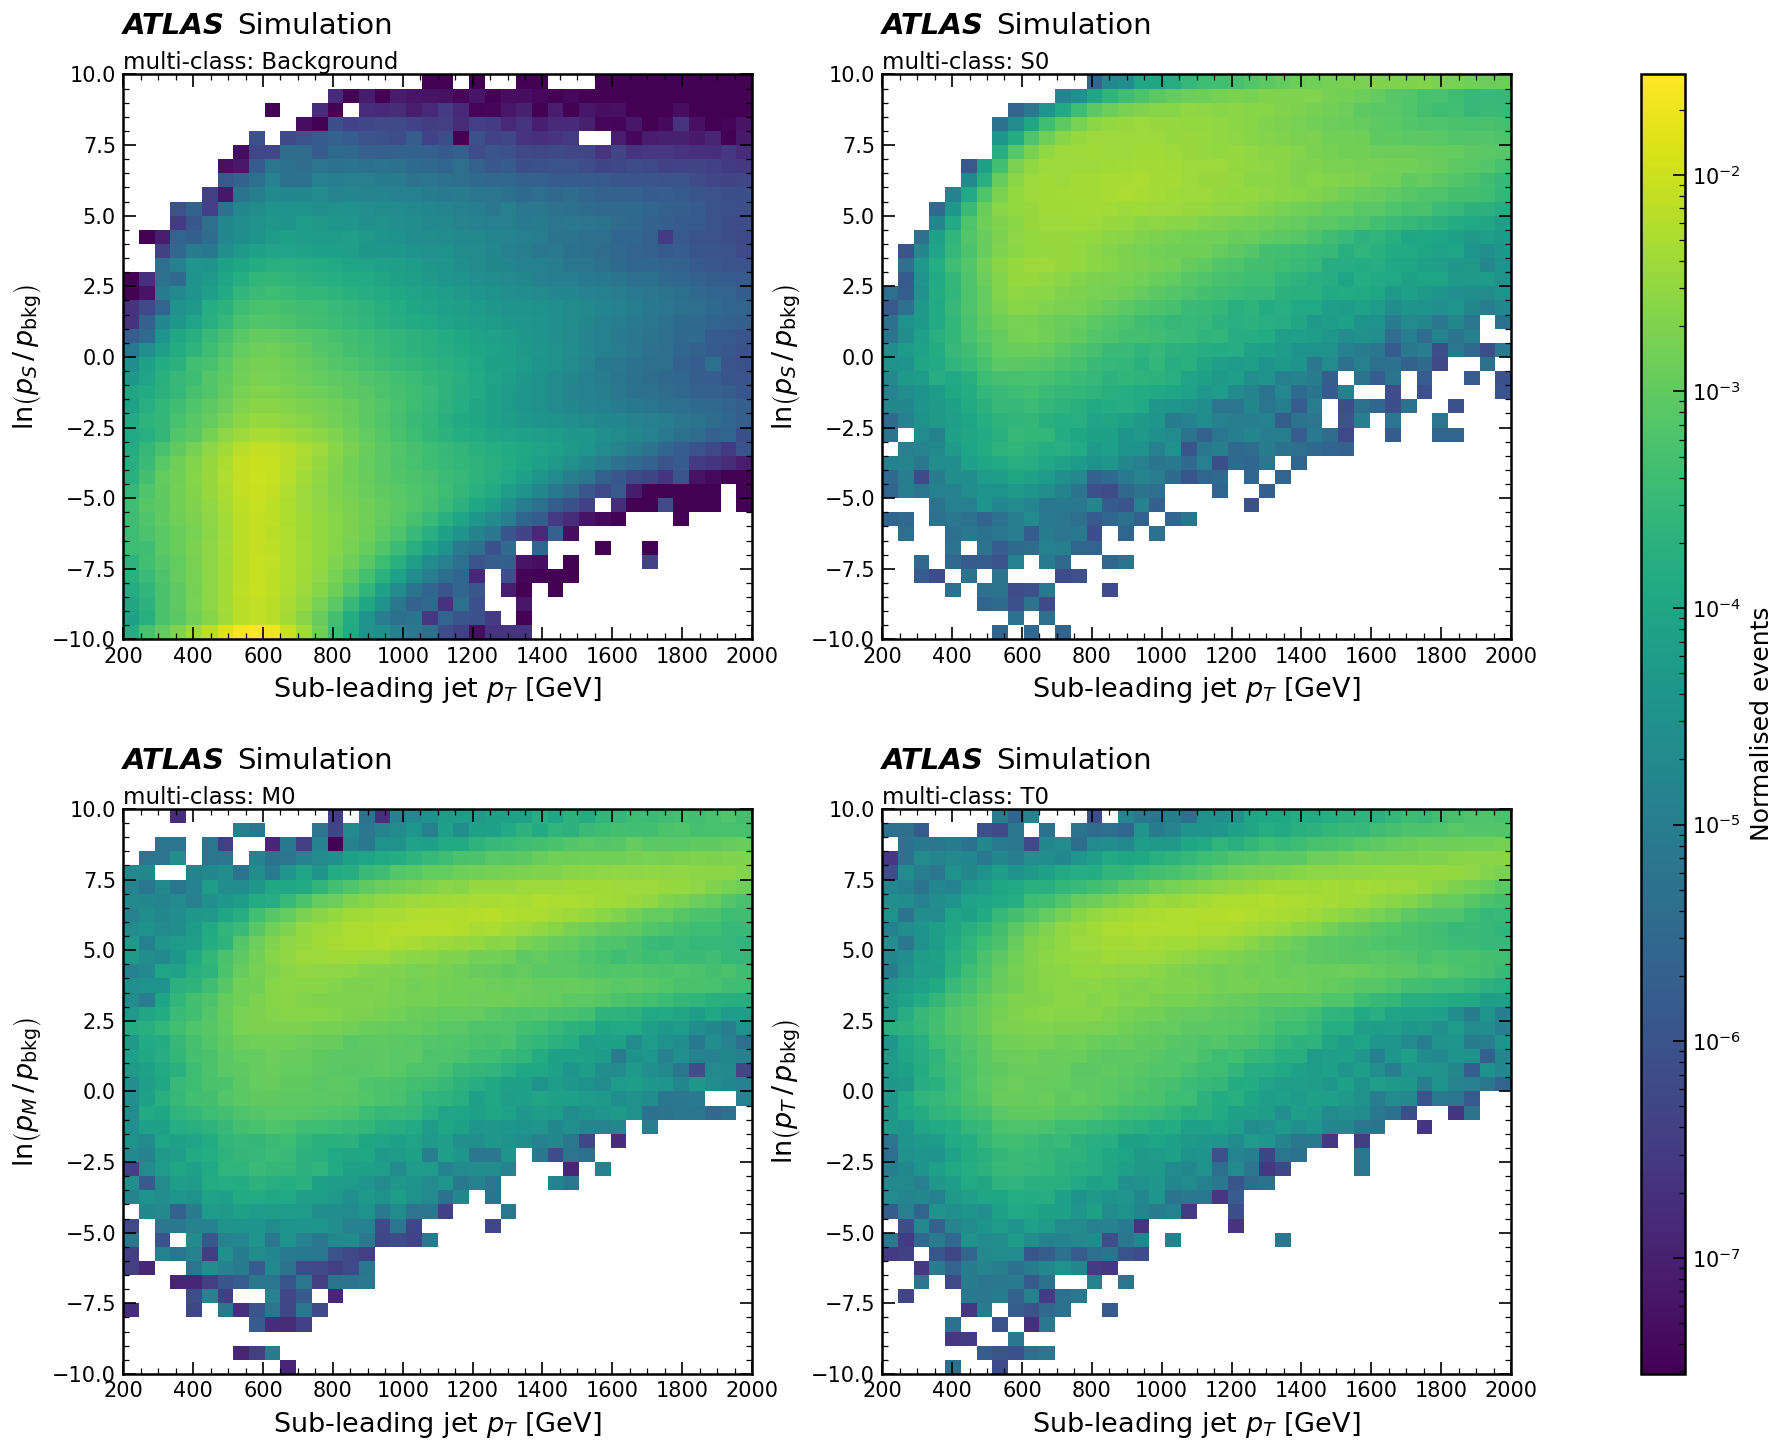
\includegraphics[width=\textwidth]{combined_var_disc-vbfrnn-v3-equal-signal-crosssection/mc01_combined_SigJet2_pT_NOSYS.png}
\caption{Sub-leading $p_T$.}
\end{subfigure}

\medskip

\begin{subfigure}[b]{0.38\textwidth}
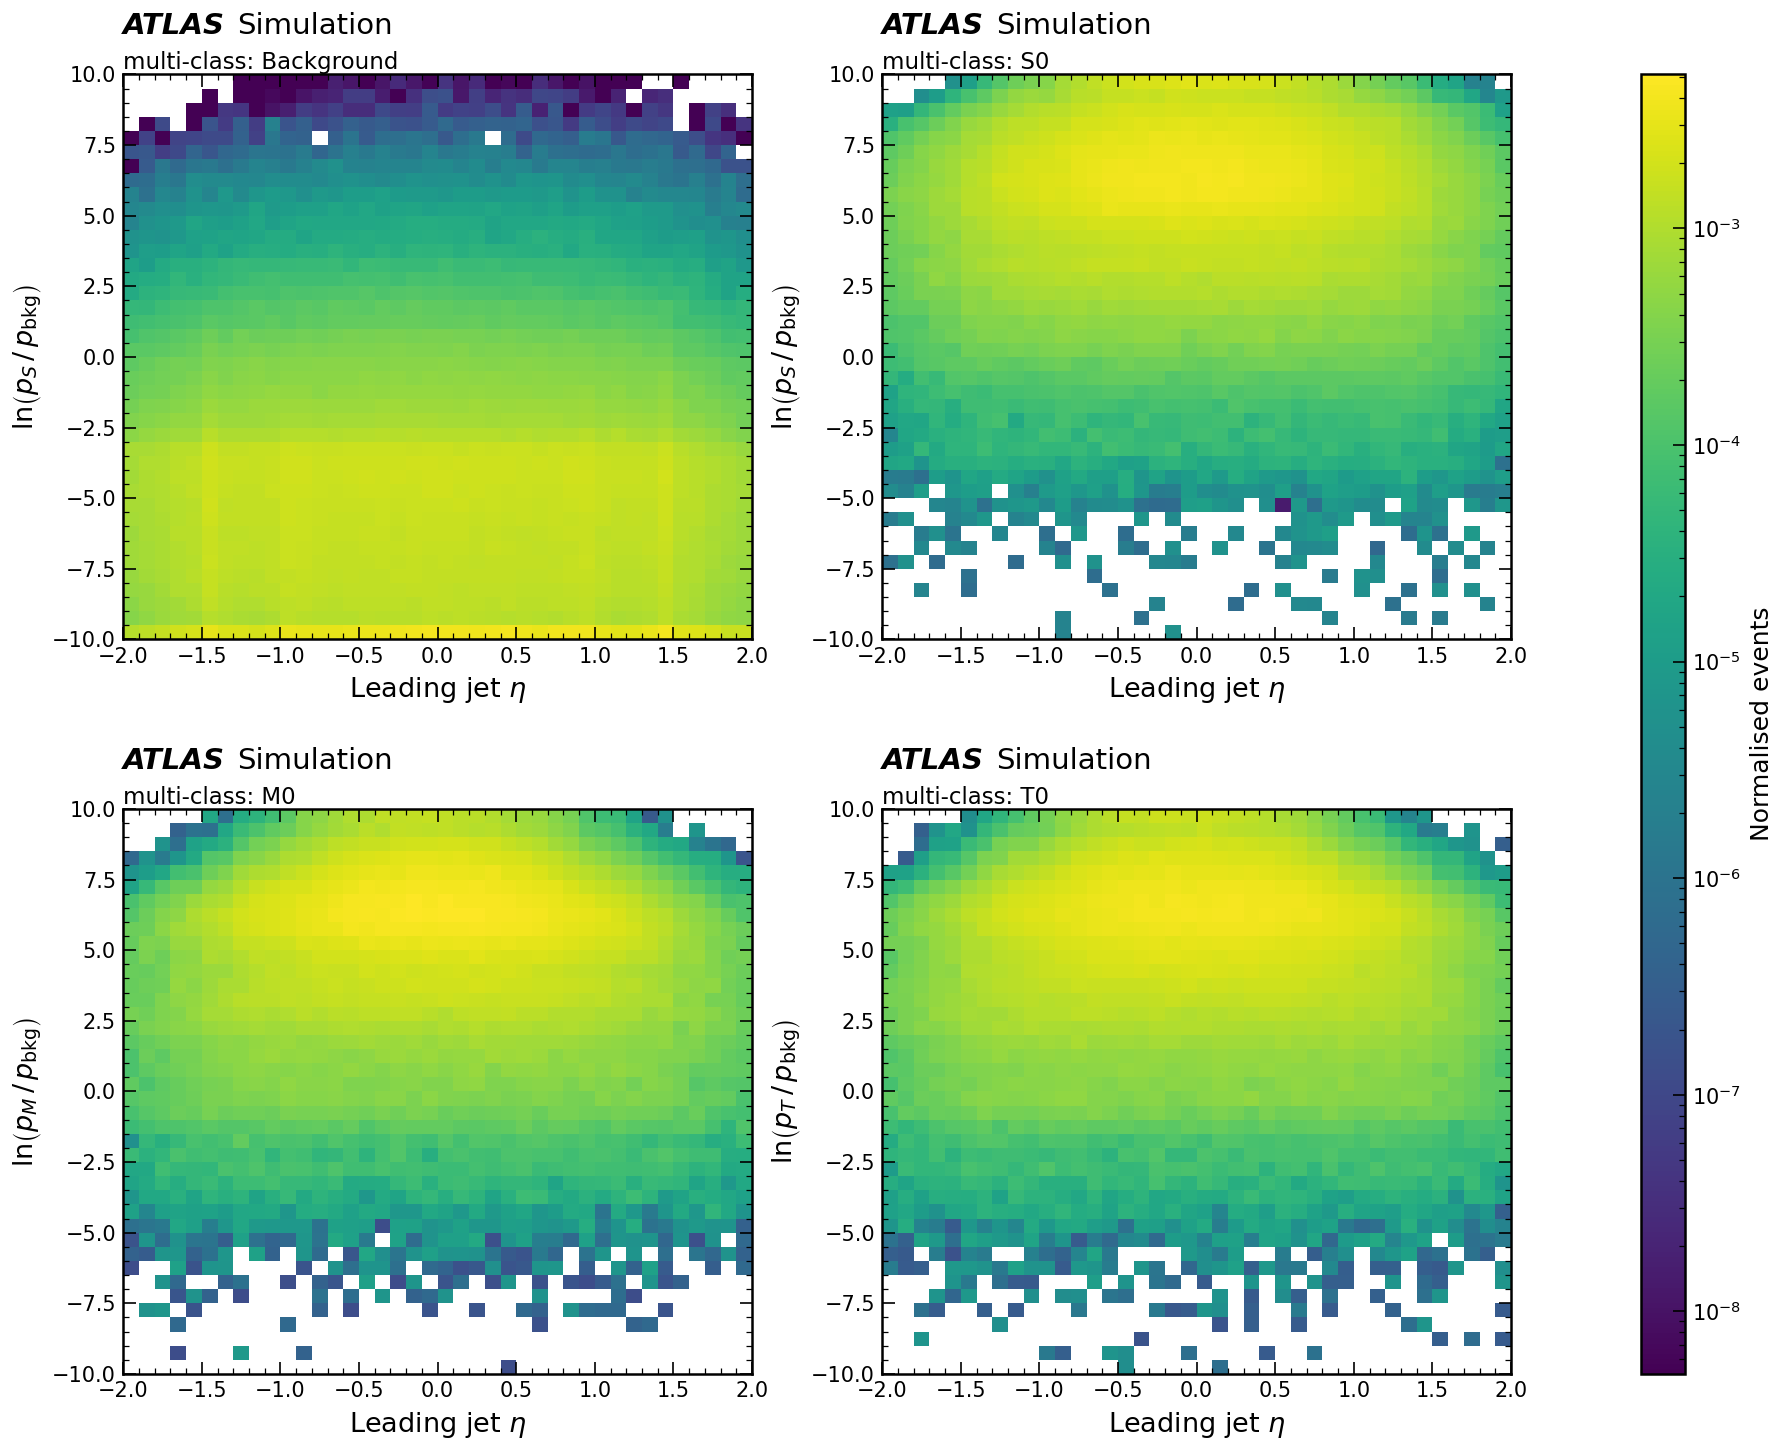
\includegraphics[width=\textwidth]{combined_var_disc-vbfrnn-v3-equal-signal-crosssection/mc01_combined_SigJet1_eta_NOSYS.png}
\caption{Leading $\eta$.}
\end{subfigure}
\hfill
\begin{subfigure}[b]{0.38\textwidth}
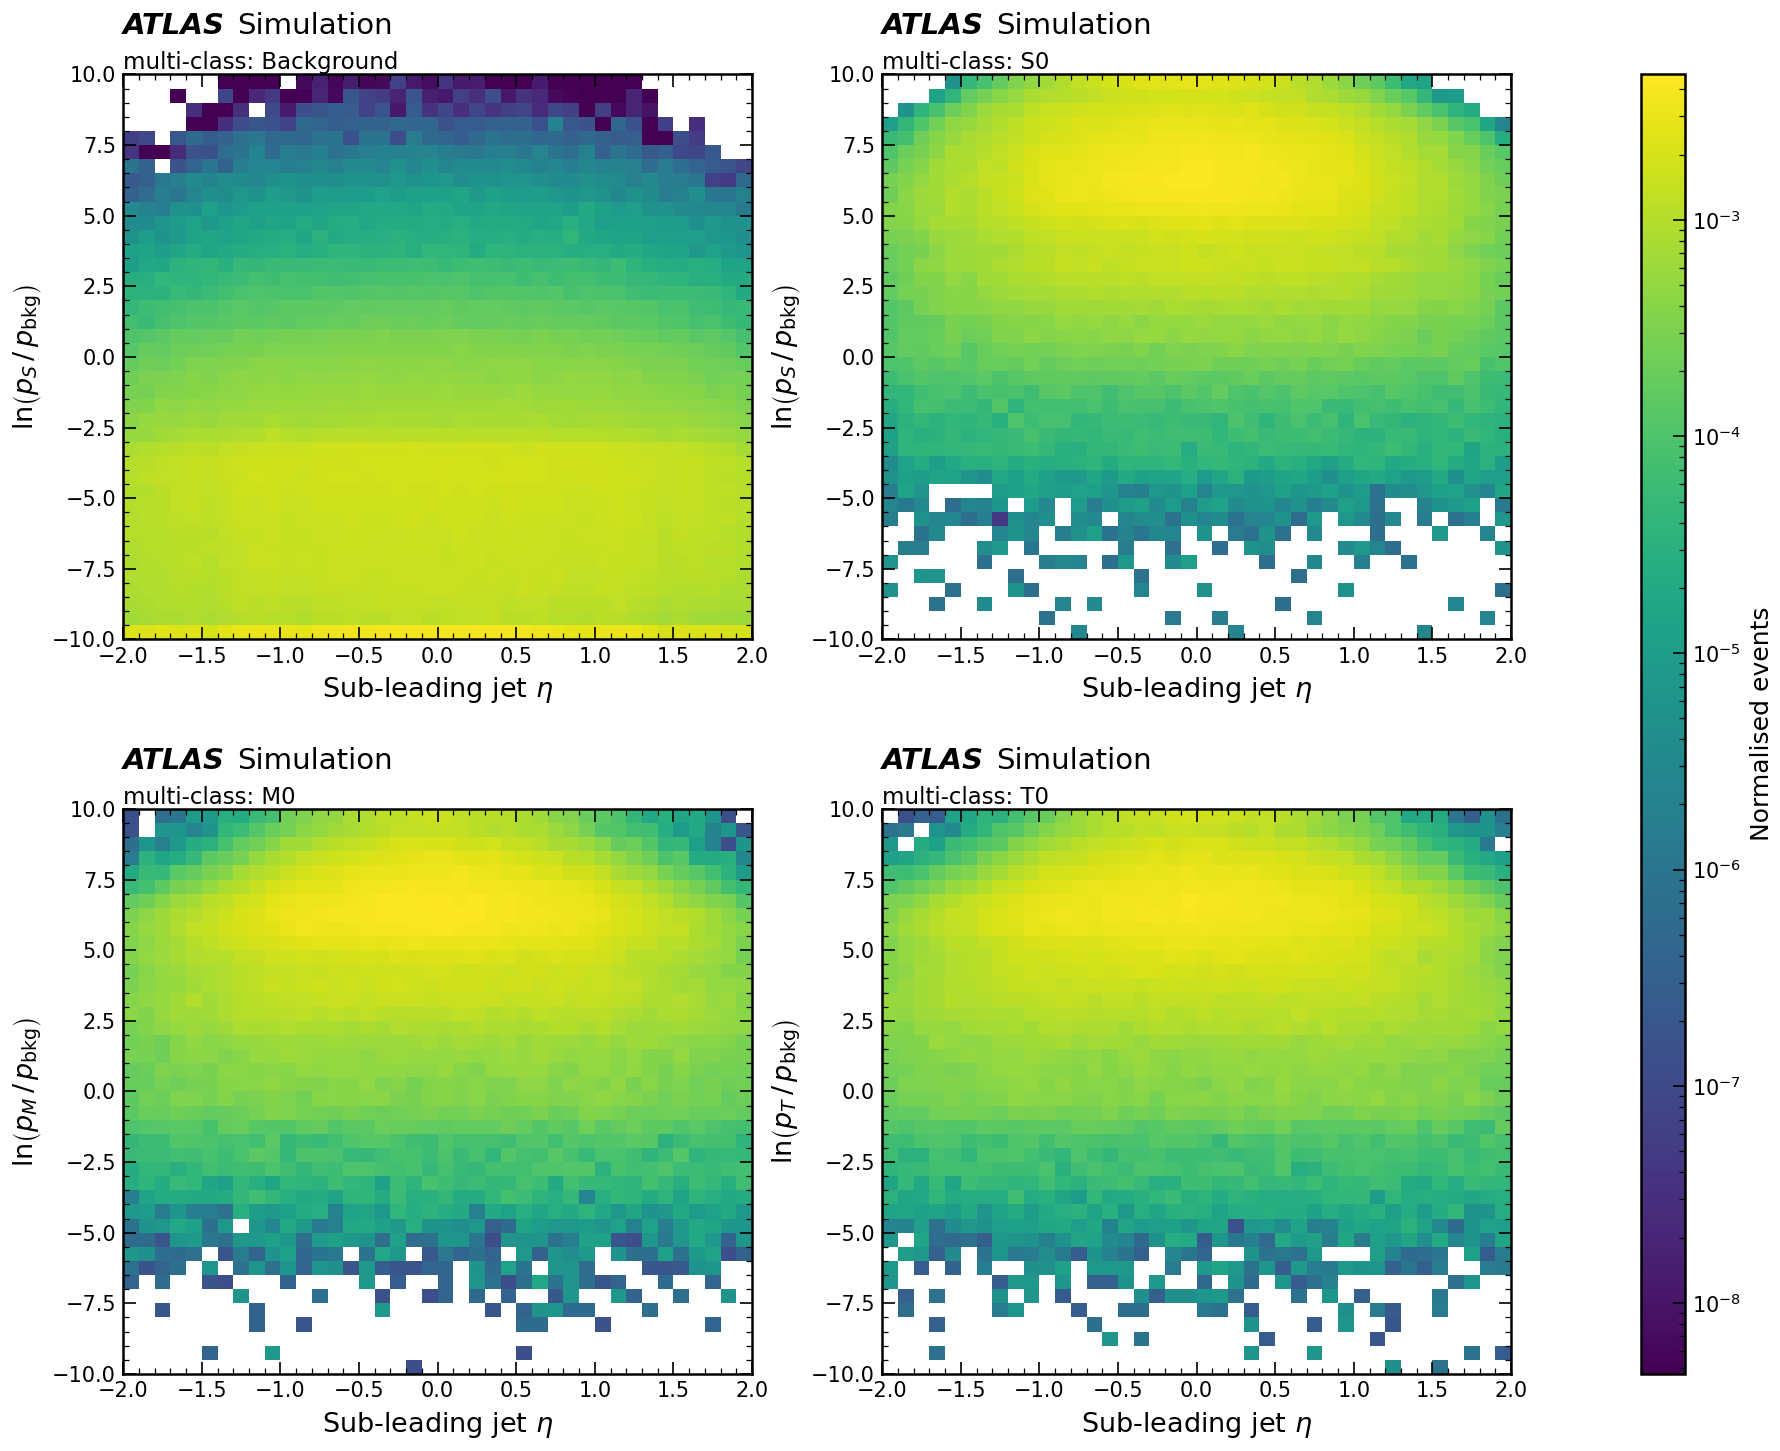
\includegraphics[width=\textwidth]{combined_var_disc-vbfrnn-v3-equal-signal-crosssection/mc01_combined_SigJet2_eta_NOSYS.png}
\caption{Sub-leading $\eta$.}
\end{subfigure}
\caption{2D distribution of the multi-class discriminant using the v3~+~equal-$\sigma$ version.}
\label{fig:app_corr_mc}
\end{figure}

\chapter{Per-operator discriminant distributions}
\label{app:templates_v3eq}

The following figures show the binned multivariate discriminant templates for every probed operator not displayed in Section~\ref{sec:sens_discriminants}, on the v3~+~equal-$\sigma$ configuration. Each panel uses the same hatched $30\%$ Gaussian background uncertainty band as the main-text discriminant figures.

\begin{figure}[htbp]
\centering
\begin{subfigure}[b]{0.32\textwidth}
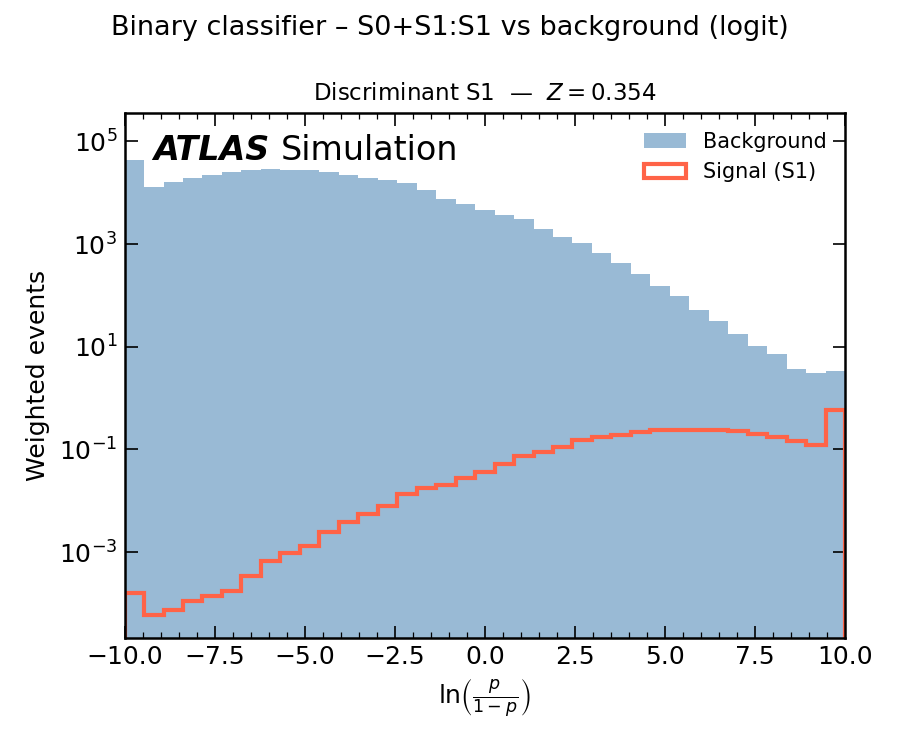
\includegraphics[width=\textwidth]{significance_plots-vbfrnn-v3-equal-signal-crosssection/binary_groups/binary_discriminants_S0_S1_S1.png}
\caption{$S_1$, specialised.}
\end{subfigure}
\hfill
\begin{subfigure}[b]{0.32\textwidth}
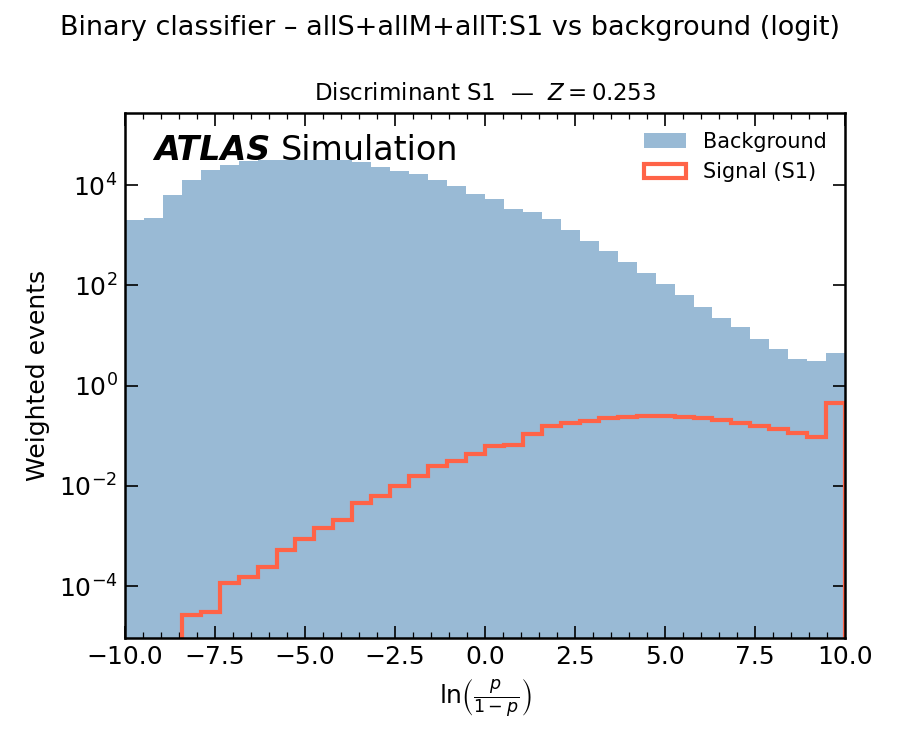
\includegraphics[width=\textwidth]{significance_plots-vbfrnn-v3-equal-signal-crosssection/binary_groups/binary_discriminants_allS_allM_allT_S1.png}
\caption{$S_1$, global.}
\end{subfigure}
\hfill
\begin{subfigure}[b]{0.32\textwidth}
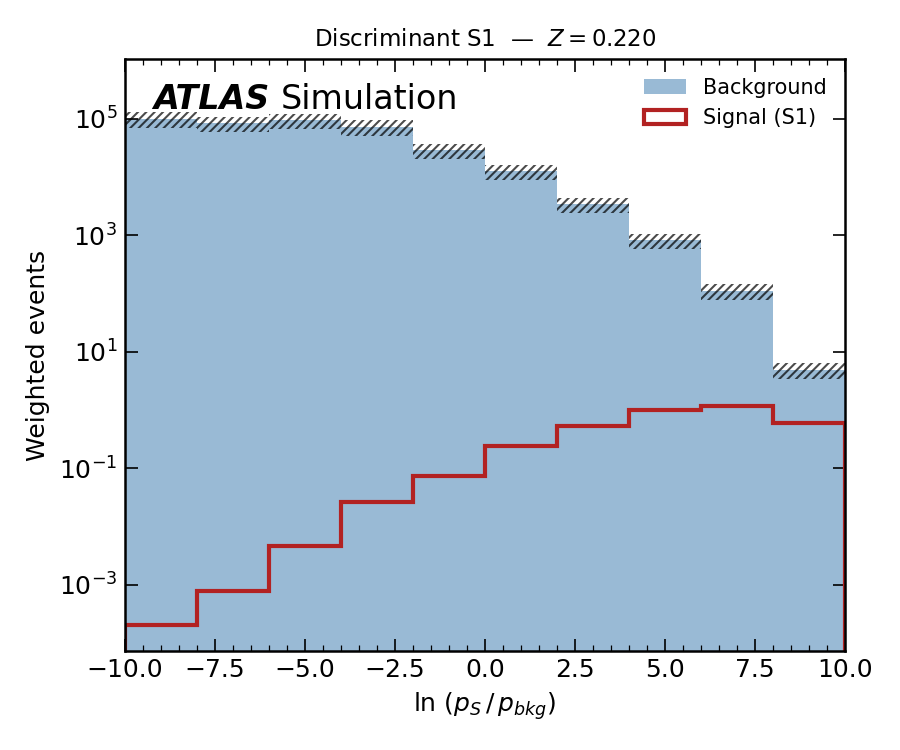
\includegraphics[width=\textwidth]{significance_plots-vbfrnn-v3-equal-signal-crosssection/multiclass/multiclass_discriminants_all_S1.png}
\caption{$S_1$, multi-class.}
\end{subfigure}
\caption{Binned multivariate discriminant for the scalar operator $S_1$ on the v3~+~equal-$\sigma$ configuration, for the three discriminant architectures.}
\label{fig:app_disc_v3eq_S}
\end{figure}

\begin{figure}[htbp]
\centering
\begin{subfigure}[b]{0.32\textwidth}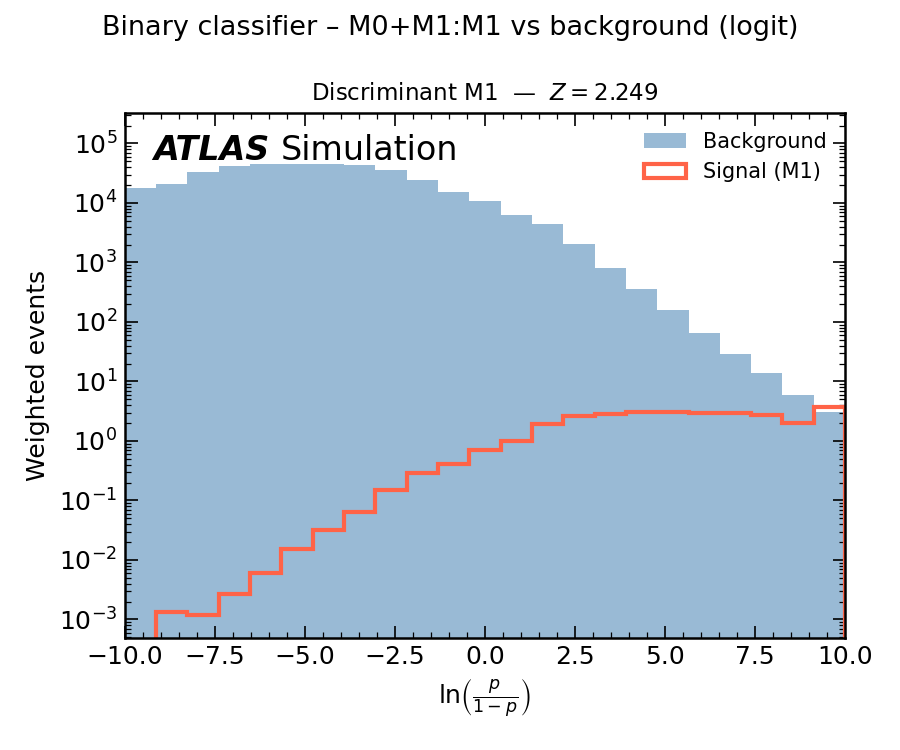
\includegraphics[width=\textwidth]{significance_plots-vbfrnn-v3-equal-signal-crosssection/binary_groups/binary_discriminants_M0_M1_M1.png}\caption{$M_1$.}\end{subfigure}\hfill
\begin{subfigure}[b]{0.32\textwidth}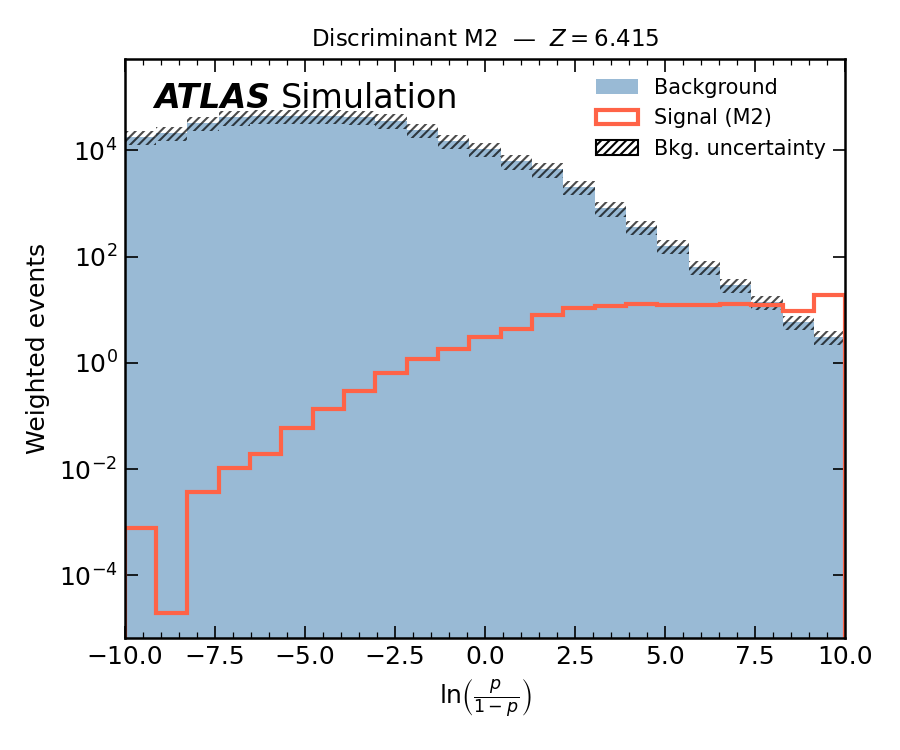
\includegraphics[width=\textwidth]{significance_plots-vbfrnn-v3-equal-signal-crosssection/binary_groups/binary_discriminants_M0_M1_M2.png}\caption{$M_2$.}\end{subfigure}\hfill
\begin{subfigure}[b]{0.32\textwidth}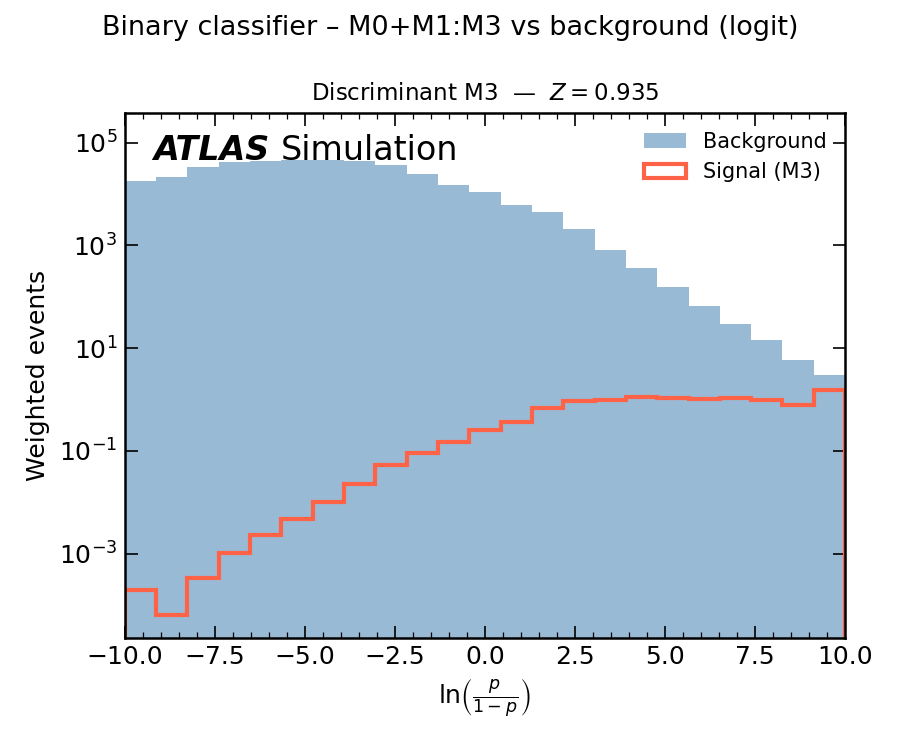
\includegraphics[width=\textwidth]{significance_plots-vbfrnn-v3-equal-signal-crosssection/binary_groups/binary_discriminants_M0_M1_M3.png}\caption{$M_3$.}\end{subfigure}

\medskip

\begin{subfigure}[b]{0.32\textwidth}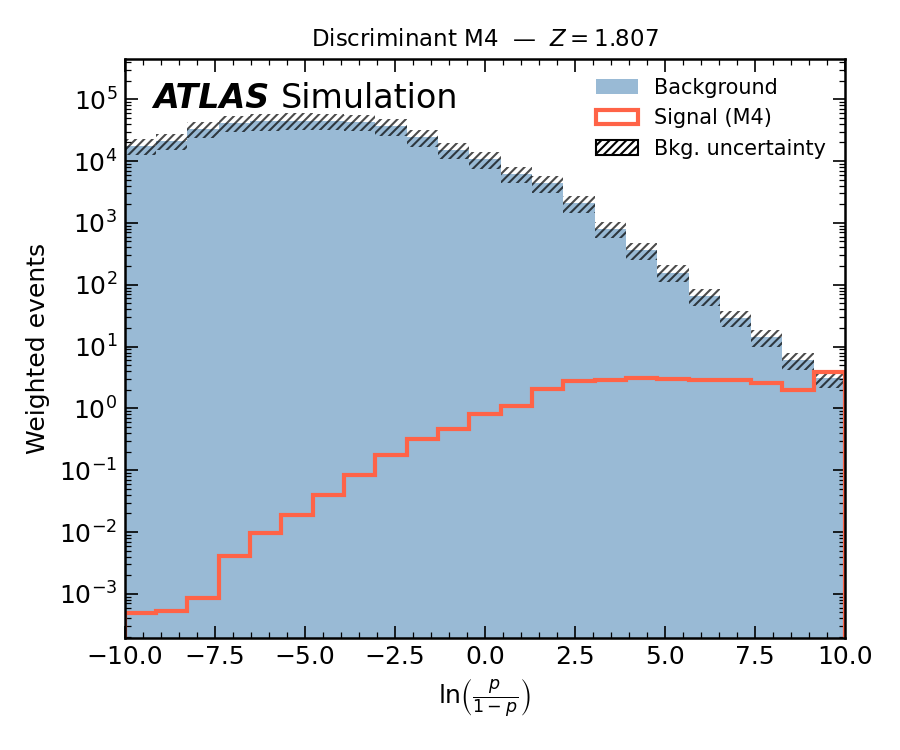
\includegraphics[width=\textwidth]{significance_plots-vbfrnn-v3-equal-signal-crosssection/binary_groups/binary_discriminants_M0_M1_M4.png}\caption{$M_4$.}\end{subfigure}\hfill
\begin{subfigure}[b]{0.32\textwidth}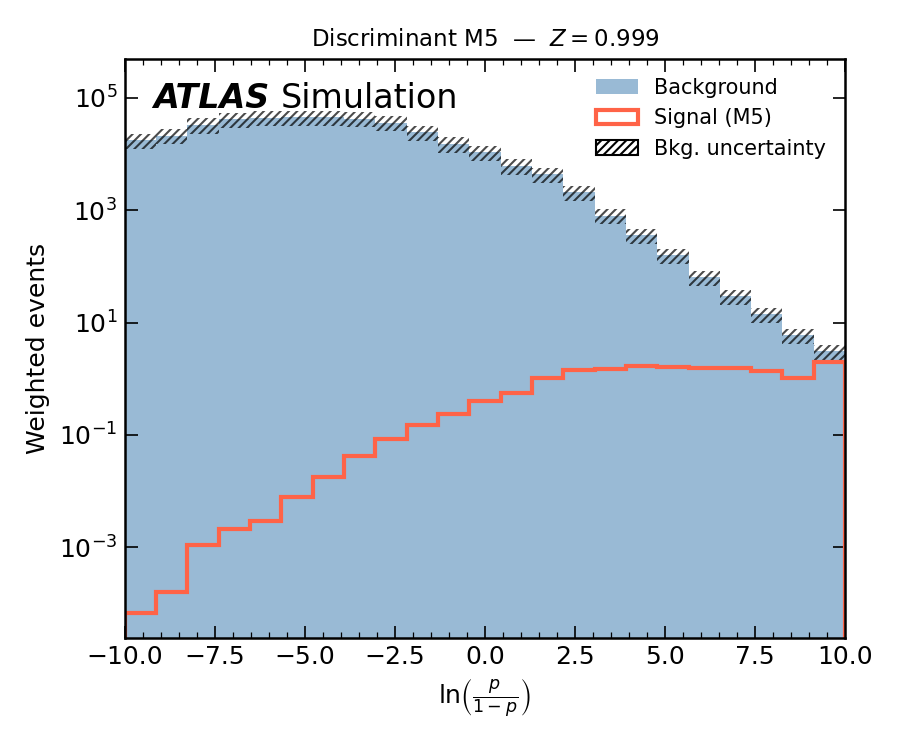
\includegraphics[width=\textwidth]{significance_plots-vbfrnn-v3-equal-signal-crosssection/binary_groups/binary_discriminants_M0_M1_M5.png}\caption{$M_5$.}\end{subfigure}\hfill
\begin{subfigure}[b]{0.32\textwidth}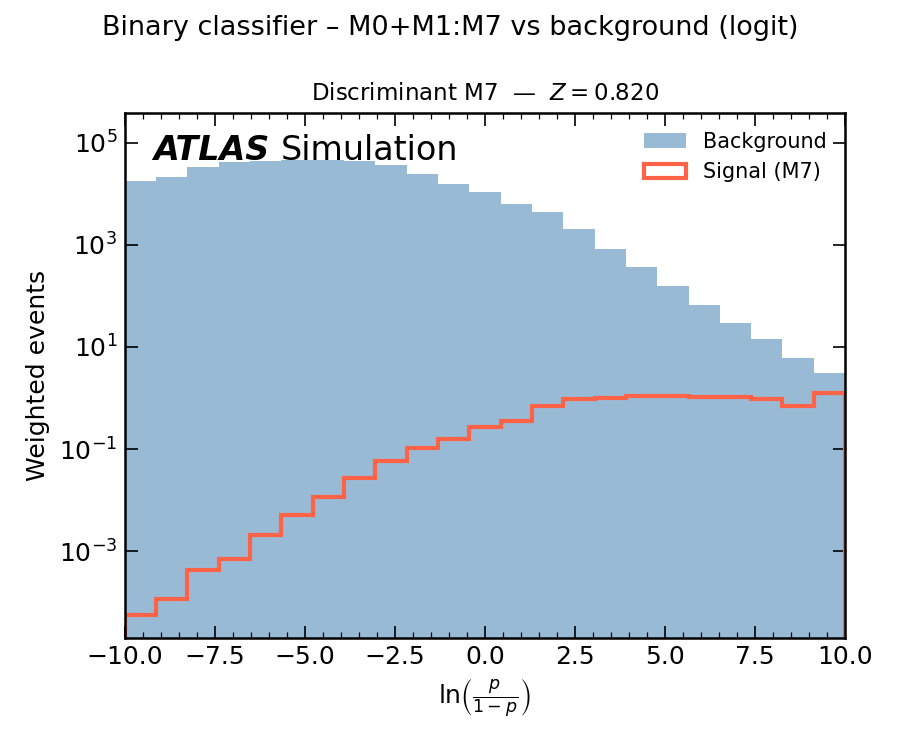
\includegraphics[width=\textwidth]{significance_plots-vbfrnn-v3-equal-signal-crosssection/binary_groups/binary_discriminants_M0_M1_M7.png}\caption{$M_7$.}\end{subfigure}
\caption{Specialised binary discriminant on the v3~+~equal-$\sigma$ configuration for the mixed operators.}
\label{fig:app_disc_v3eq_spec_M}
\end{figure}

\begin{figure}[htbp]
\centering
\begin{subfigure}[b]{0.32\textwidth}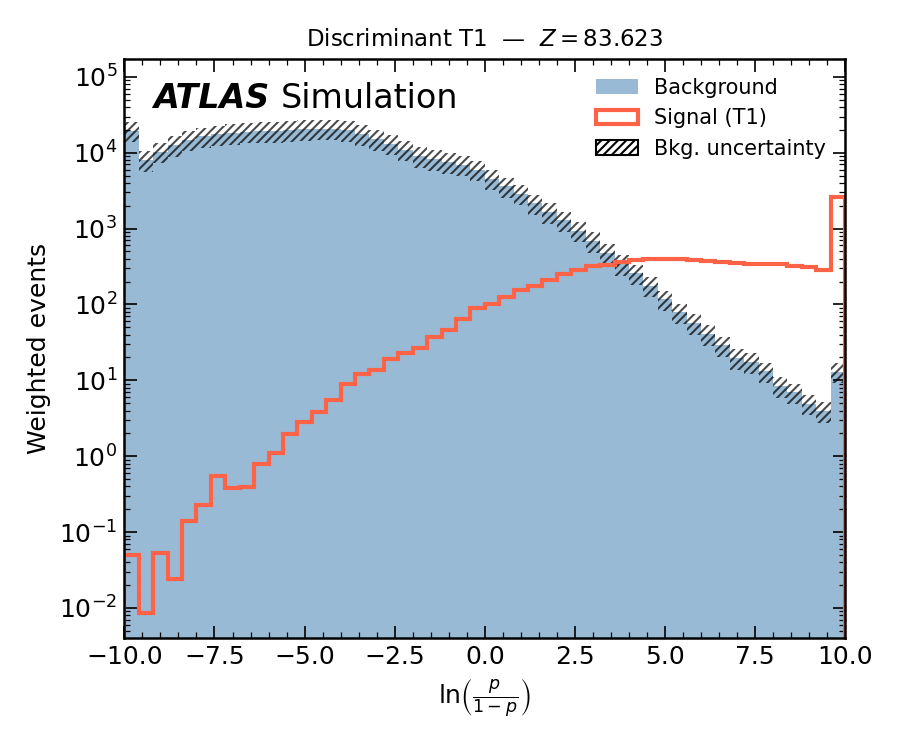
\includegraphics[width=\textwidth]{significance_plots-vbfrnn-v3-equal-signal-crosssection/binary_groups/binary_discriminants_T0_T1_T1.png}\caption{$T_1$.}\end{subfigure}\hfill
\begin{subfigure}[b]{0.32\textwidth}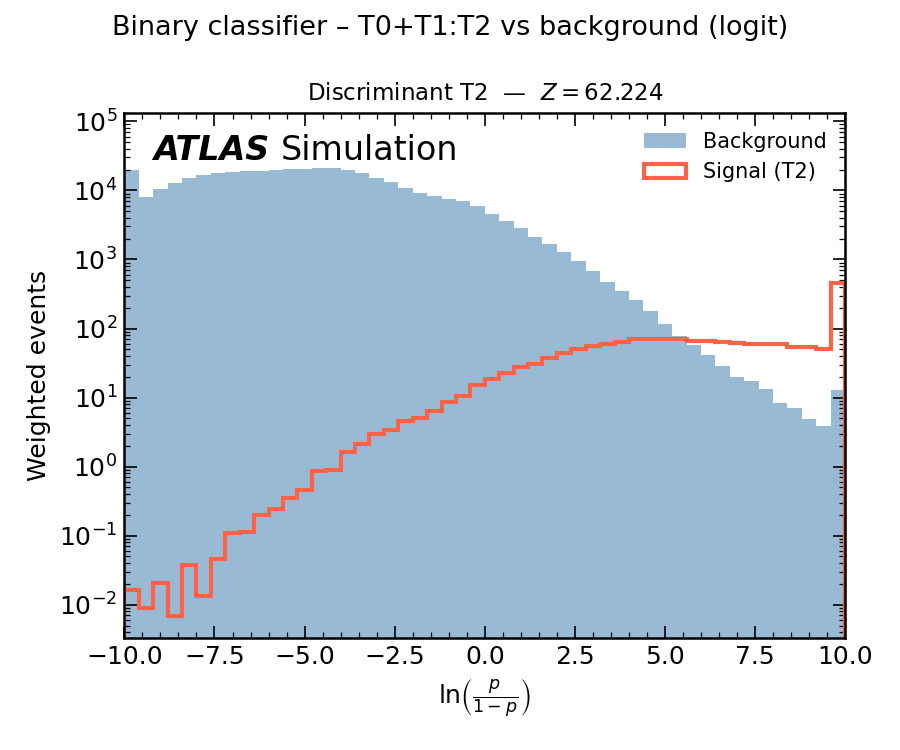
\includegraphics[width=\textwidth]{significance_plots-vbfrnn-v3-equal-signal-crosssection/binary_groups/binary_discriminants_T0_T1_T2.png}\caption{$T_2$.}\end{subfigure}\hfill
\begin{subfigure}[b]{0.32\textwidth}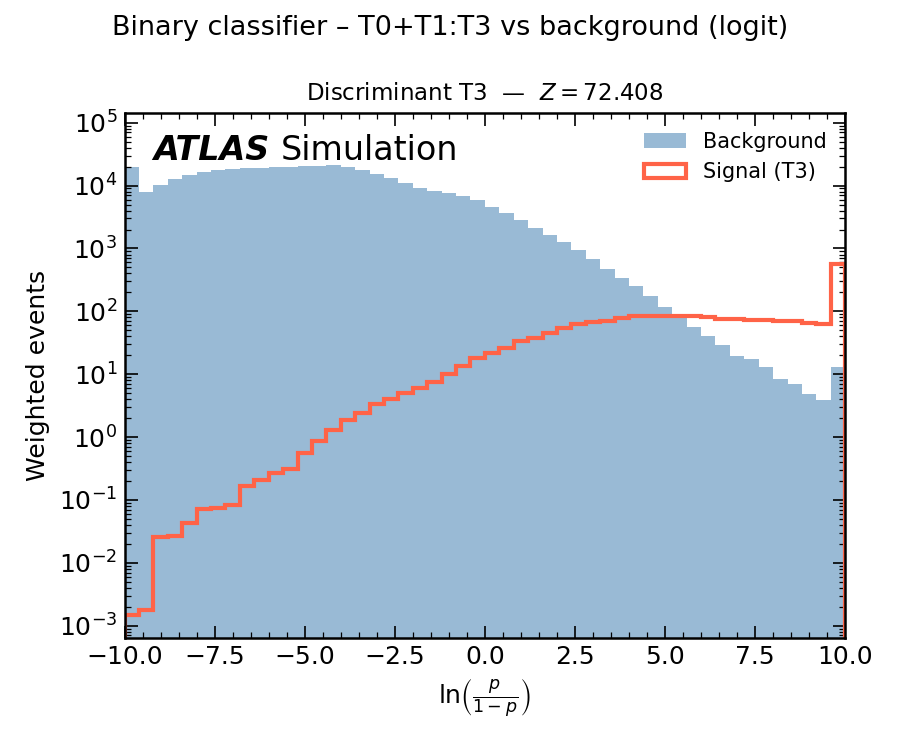
\includegraphics[width=\textwidth]{significance_plots-vbfrnn-v3-equal-signal-crosssection/binary_groups/binary_discriminants_T0_T1_T3.png}\caption{$T_3$.}\end{subfigure}

\medskip

\begin{subfigure}[b]{0.32\textwidth}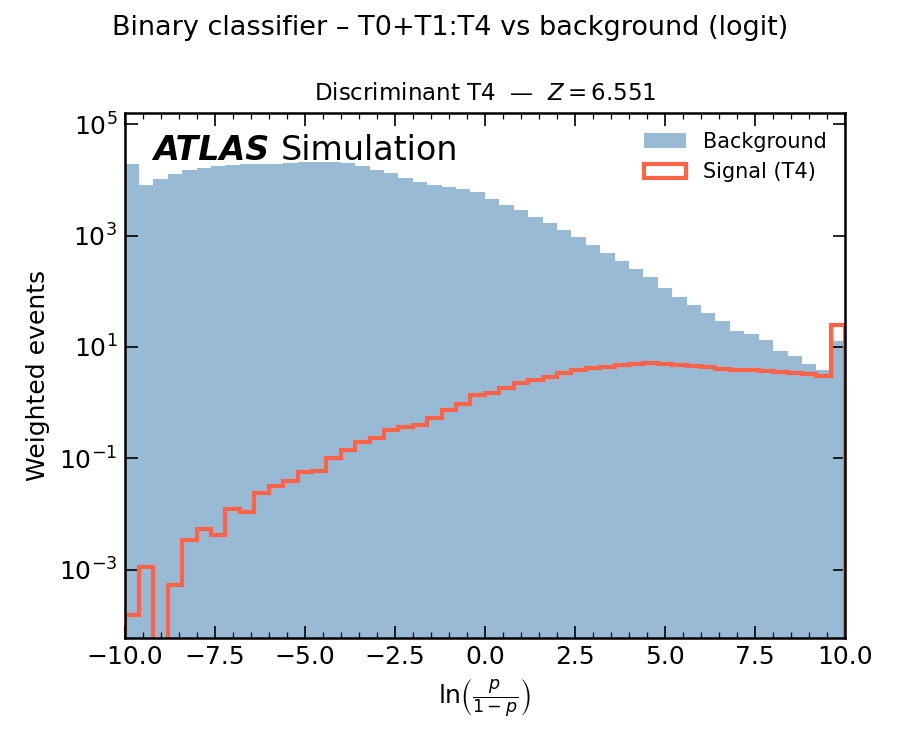
\includegraphics[width=\textwidth]{significance_plots-vbfrnn-v3-equal-signal-crosssection/binary_groups/binary_discriminants_T0_T1_T4.png}\caption{$T_4$.}\end{subfigure}\hfill
\begin{subfigure}[b]{0.32\textwidth}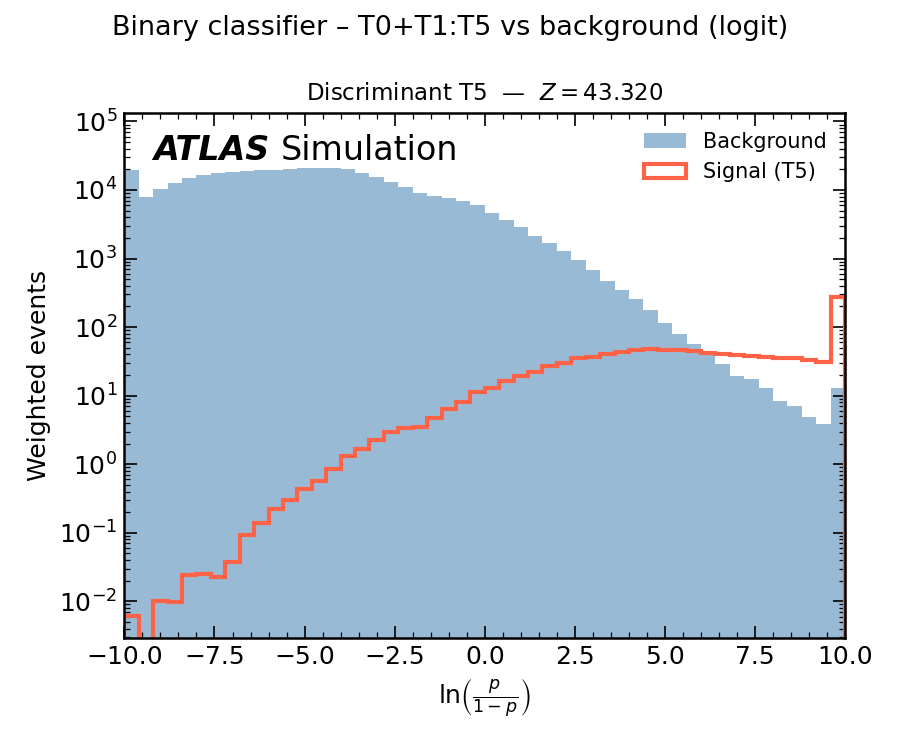
\includegraphics[width=\textwidth]{significance_plots-vbfrnn-v3-equal-signal-crosssection/binary_groups/binary_discriminants_T0_T1_T5.png}\caption{$T_5$.}\end{subfigure}\hfill
\begin{subfigure}[b]{0.32\textwidth}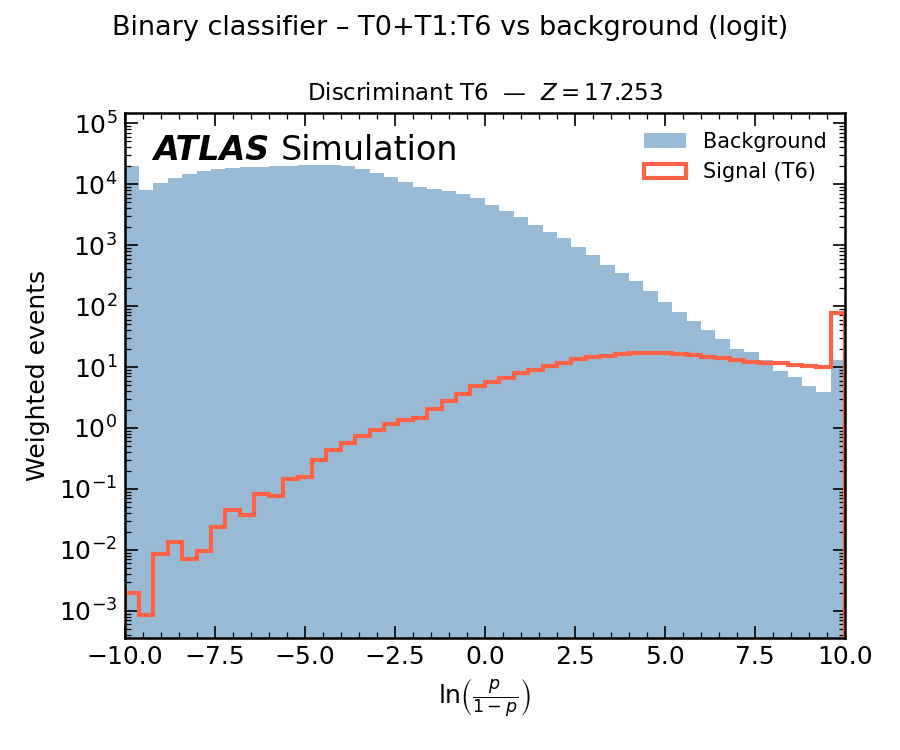
\includegraphics[width=\textwidth]{significance_plots-vbfrnn-v3-equal-signal-crosssection/binary_groups/binary_discriminants_T0_T1_T6.png}\caption{$T_6$.}\end{subfigure}

\medskip

\begin{subfigure}[b]{0.32\textwidth}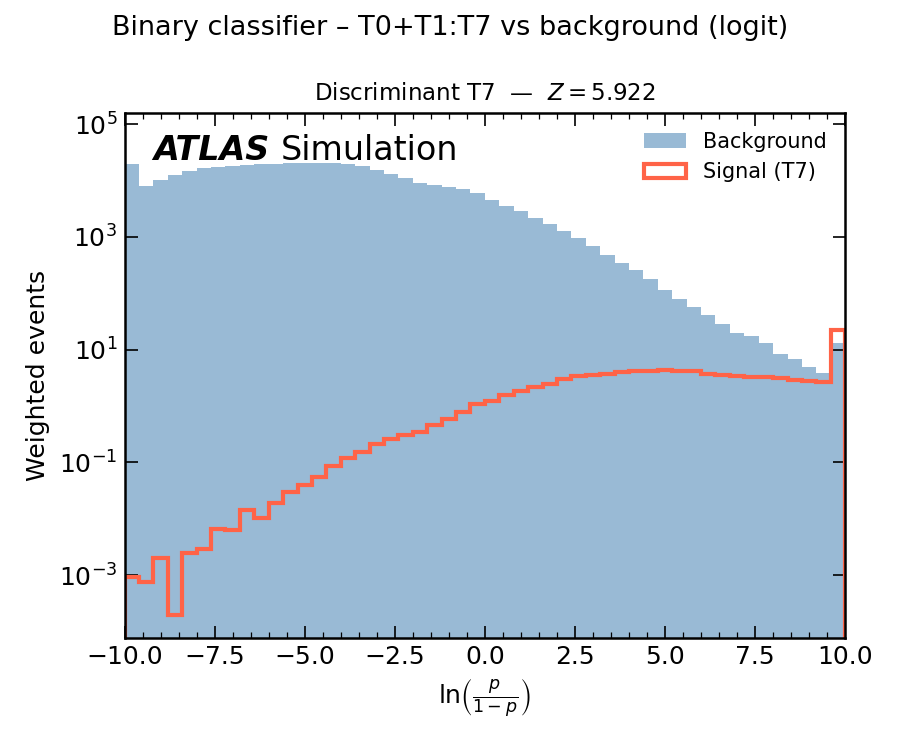
\includegraphics[width=\textwidth]{significance_plots-vbfrnn-v3-equal-signal-crosssection/binary_groups/binary_discriminants_T0_T1_T7.png}\caption{$T_7$.}\end{subfigure}\hfill
\begin{subfigure}[b]{0.32\textwidth}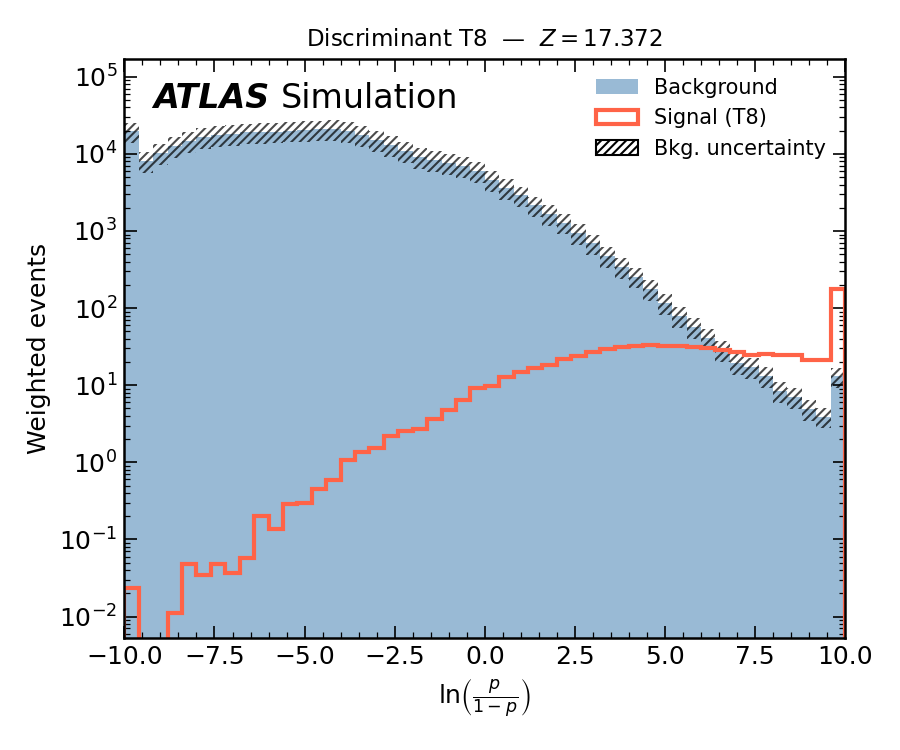
\includegraphics[width=\textwidth]{significance_plots-vbfrnn-v3-equal-signal-crosssection/binary_groups/binary_discriminants_T0_T1_T8.png}\caption{$T_8$.}\end{subfigure}\hfill
\begin{subfigure}[b]{0.32\textwidth}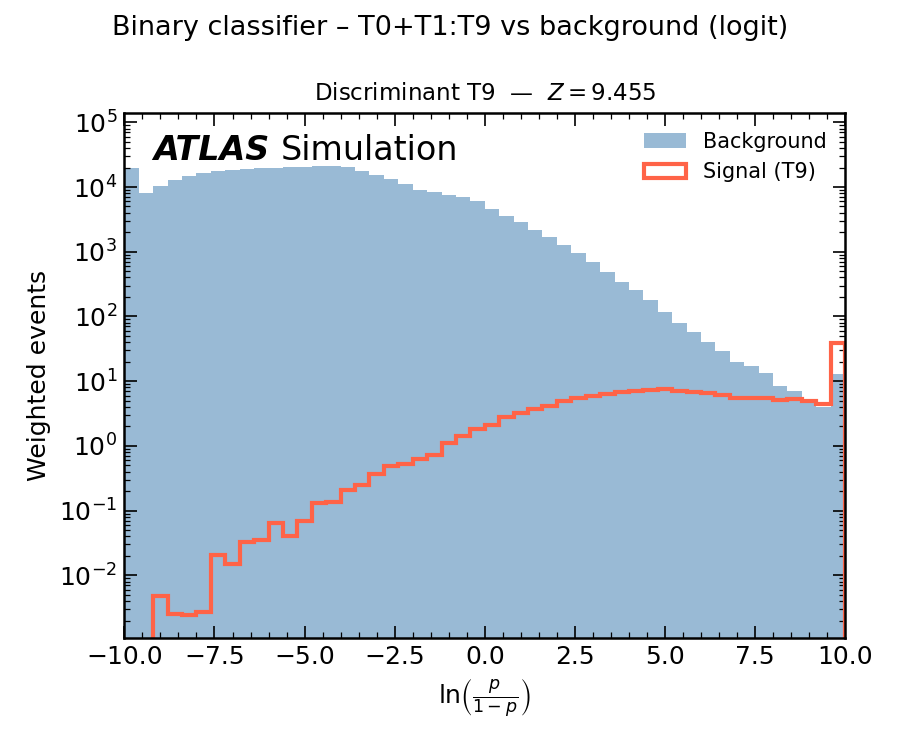
\includegraphics[width=\textwidth]{significance_plots-vbfrnn-v3-equal-signal-crosssection/binary_groups/binary_discriminants_T0_T1_T9.png}\caption{$T_9$.}\end{subfigure}
\caption{Specialised binary discriminant on the v3~+~equal-$\sigma$ configuration for the tensor operators.}
\label{fig:app_disc_v3eq_spec_T}
\end{figure}

\begin{figure}[htbp]
\centering
\begin{subfigure}[b]{0.32\textwidth}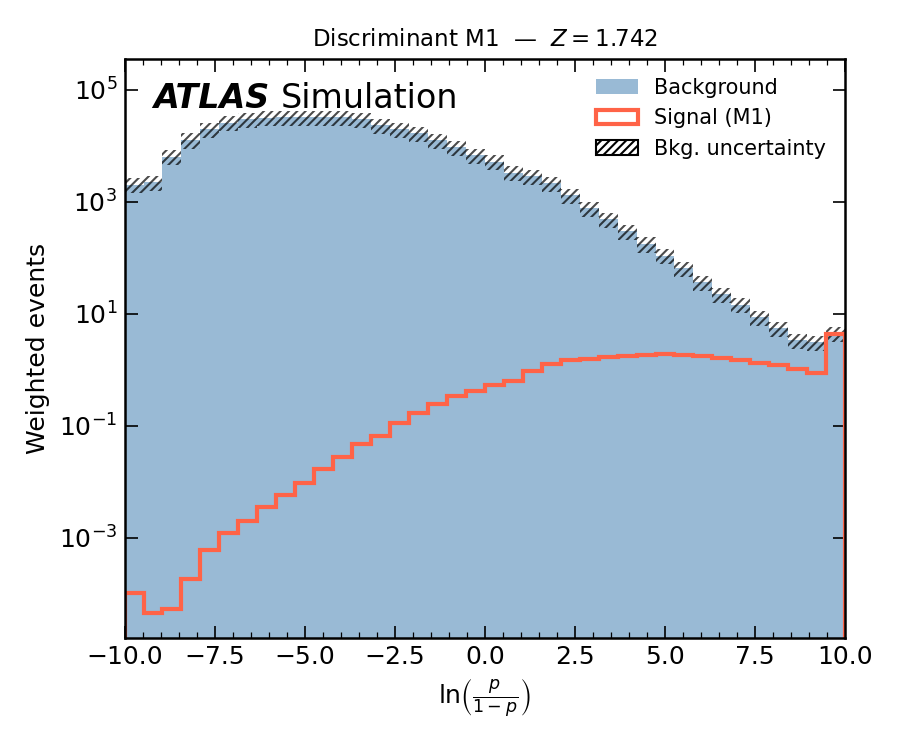
\includegraphics[width=\textwidth]{significance_plots-vbfrnn-v3-equal-signal-crosssection/binary_groups/binary_discriminants_allS_allM_allT_M1.png}\caption{$M_1$.}\end{subfigure}\hfill
\begin{subfigure}[b]{0.32\textwidth}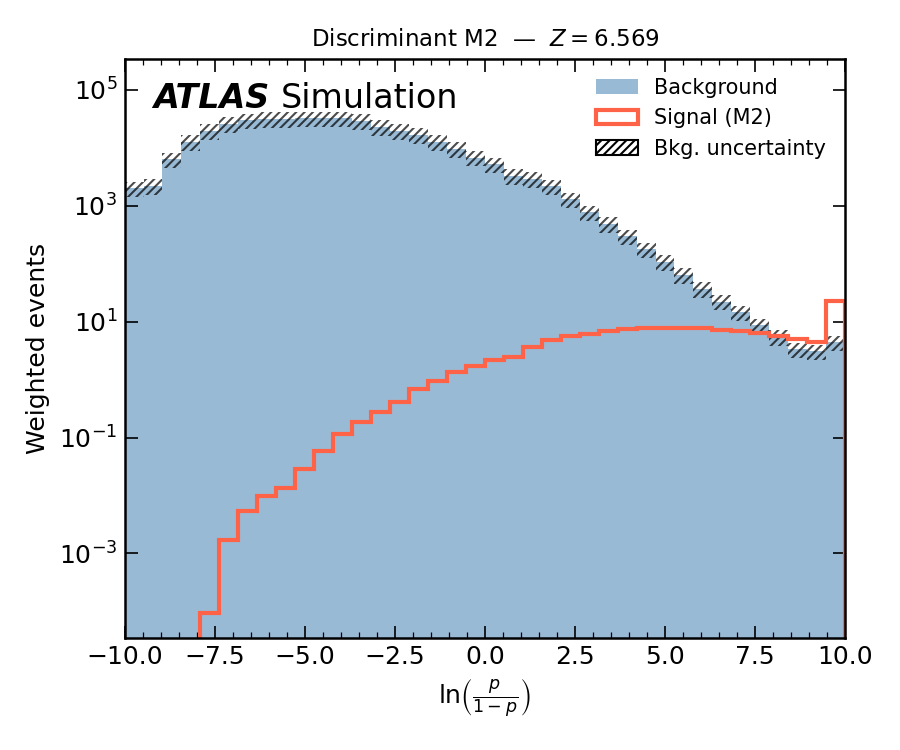
\includegraphics[width=\textwidth]{significance_plots-vbfrnn-v3-equal-signal-crosssection/binary_groups/binary_discriminants_allS_allM_allT_M2.png}\caption{$M_2$.}\end{subfigure}\hfill
\begin{subfigure}[b]{0.32\textwidth}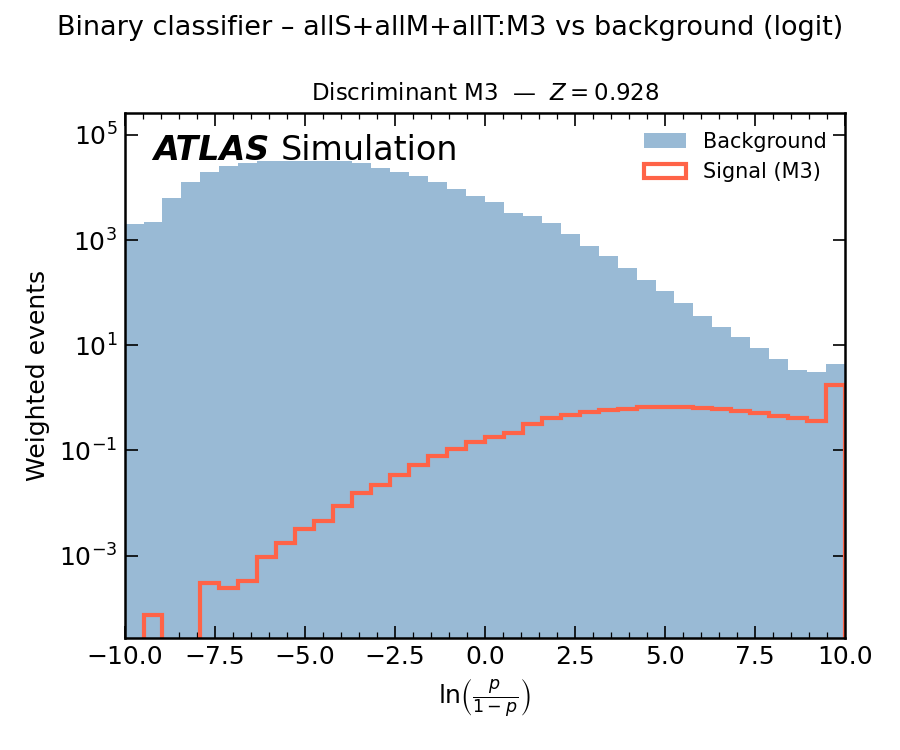
\includegraphics[width=\textwidth]{significance_plots-vbfrnn-v3-equal-signal-crosssection/binary_groups/binary_discriminants_allS_allM_allT_M3.png}\caption{$M_3$.}\end{subfigure}

\medskip

\begin{subfigure}[b]{0.32\textwidth}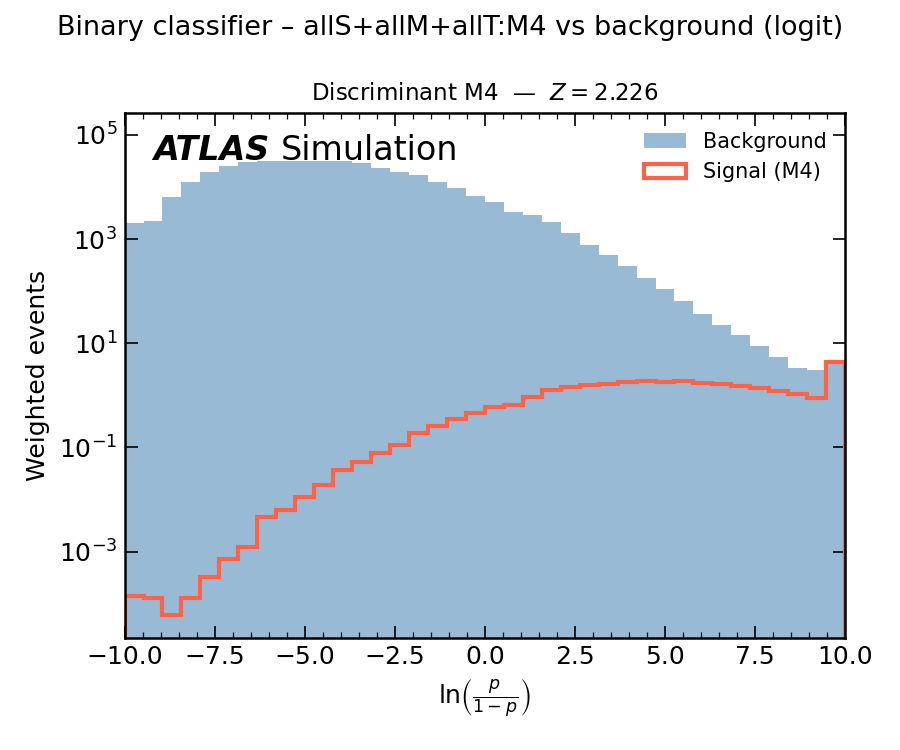
\includegraphics[width=\textwidth]{significance_plots-vbfrnn-v3-equal-signal-crosssection/binary_groups/binary_discriminants_allS_allM_allT_M4.png}\caption{$M_4$.}\end{subfigure}\hfill
\begin{subfigure}[b]{0.32\textwidth}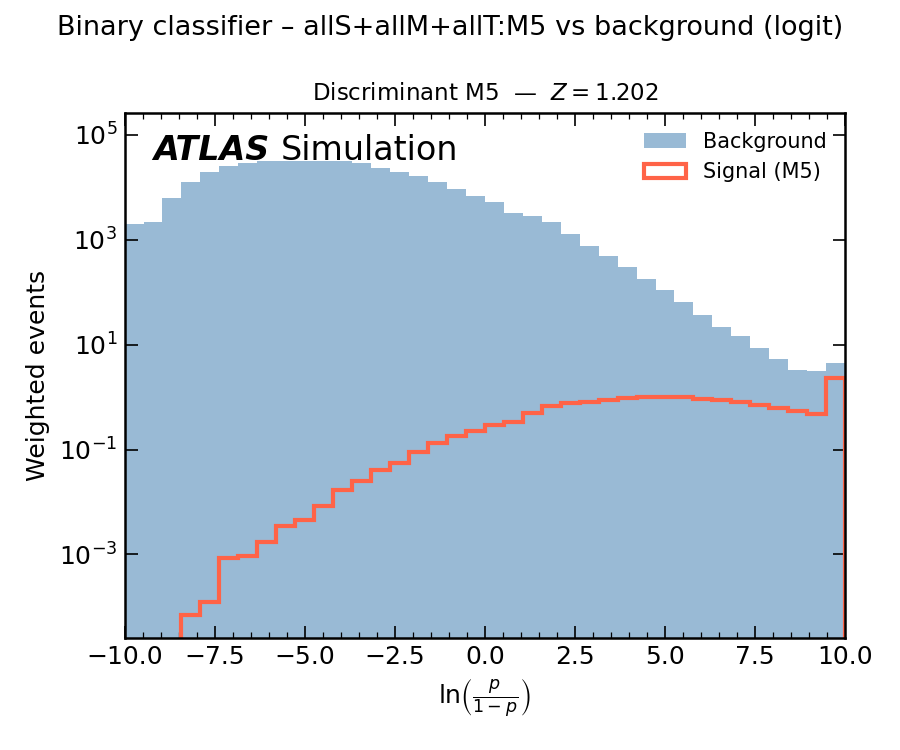
\includegraphics[width=\textwidth]{significance_plots-vbfrnn-v3-equal-signal-crosssection/binary_groups/binary_discriminants_allS_allM_allT_M5.png}\caption{$M_5$.}\end{subfigure}\hfill
\begin{subfigure}[b]{0.32\textwidth}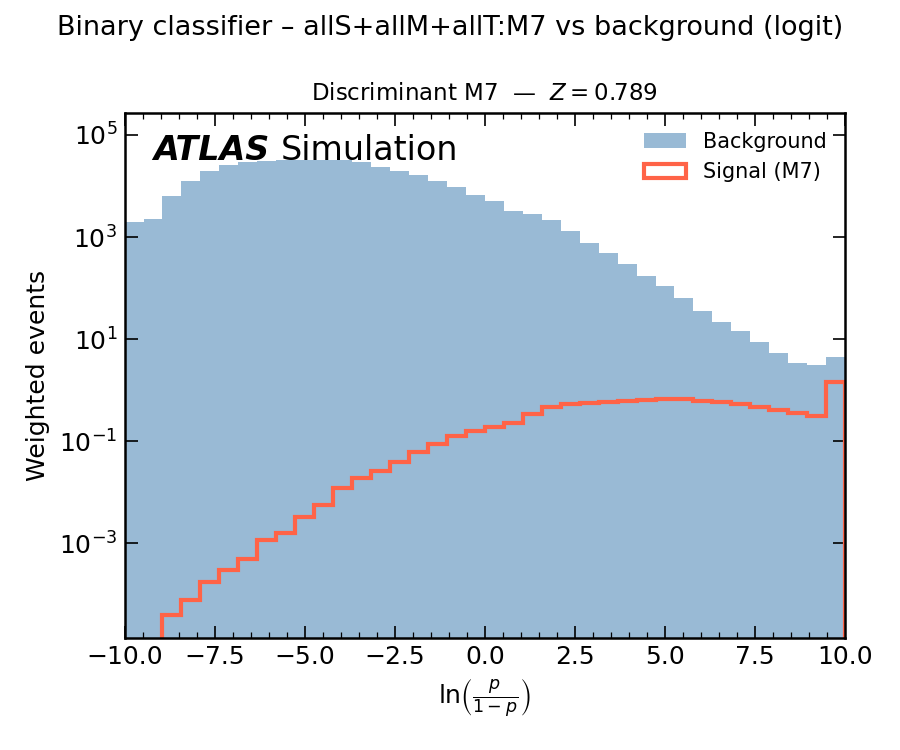
\includegraphics[width=\textwidth]{significance_plots-vbfrnn-v3-equal-signal-crosssection/binary_groups/binary_discriminants_allS_allM_allT_M7.png}\caption{$M_7$.}\end{subfigure}
\caption{Global binary discriminant on the v3~+~equal-$\sigma$ configuration for the mixed operators.}
\label{fig:app_disc_v3eq_global_M}
\end{figure}

\begin{figure}[htbp]
\centering
\begin{subfigure}[b]{0.32\textwidth}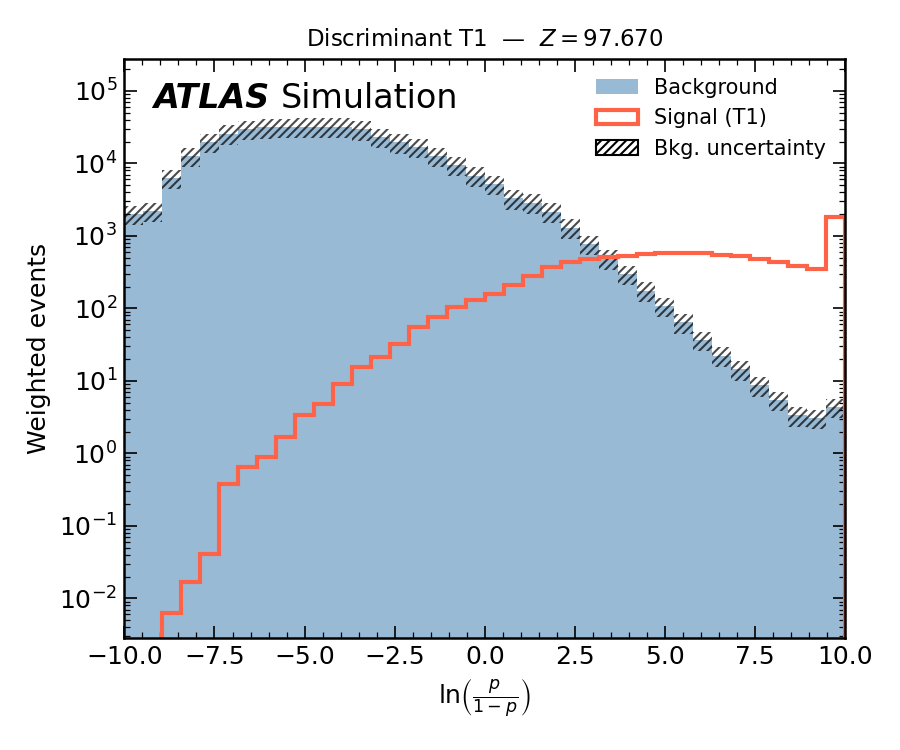
\includegraphics[width=\textwidth]{significance_plots-vbfrnn-v3-equal-signal-crosssection/binary_groups/binary_discriminants_allS_allM_allT_T1.png}\caption{$T_1$.}\end{subfigure}\hfill
\begin{subfigure}[b]{0.32\textwidth}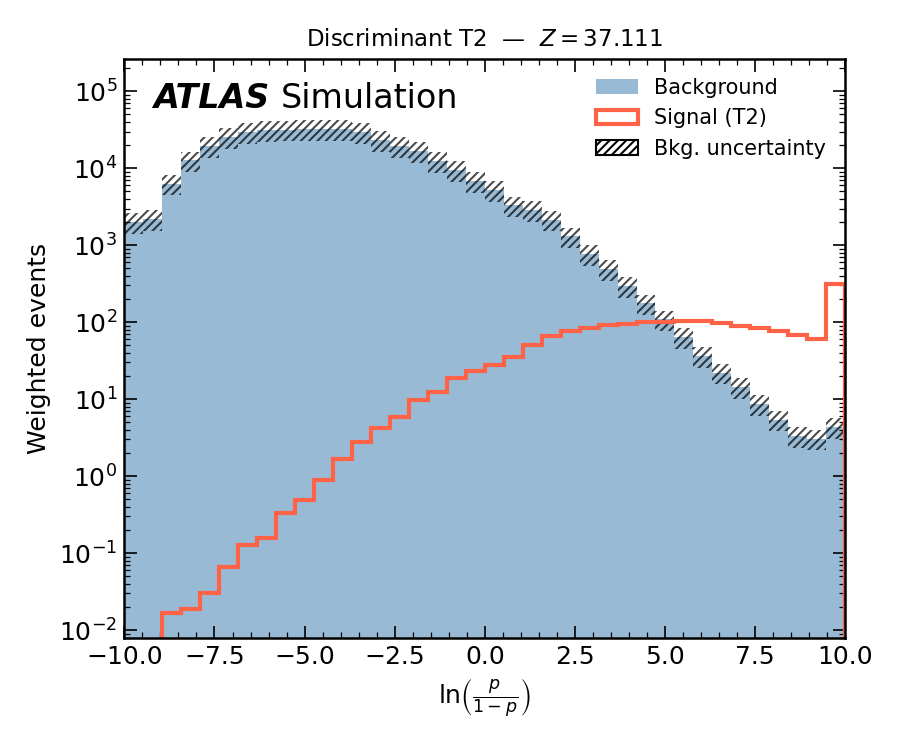
\includegraphics[width=\textwidth]{significance_plots-vbfrnn-v3-equal-signal-crosssection/binary_groups/binary_discriminants_allS_allM_allT_T2.png}\caption{$T_2$.}\end{subfigure}\hfill
\begin{subfigure}[b]{0.32\textwidth}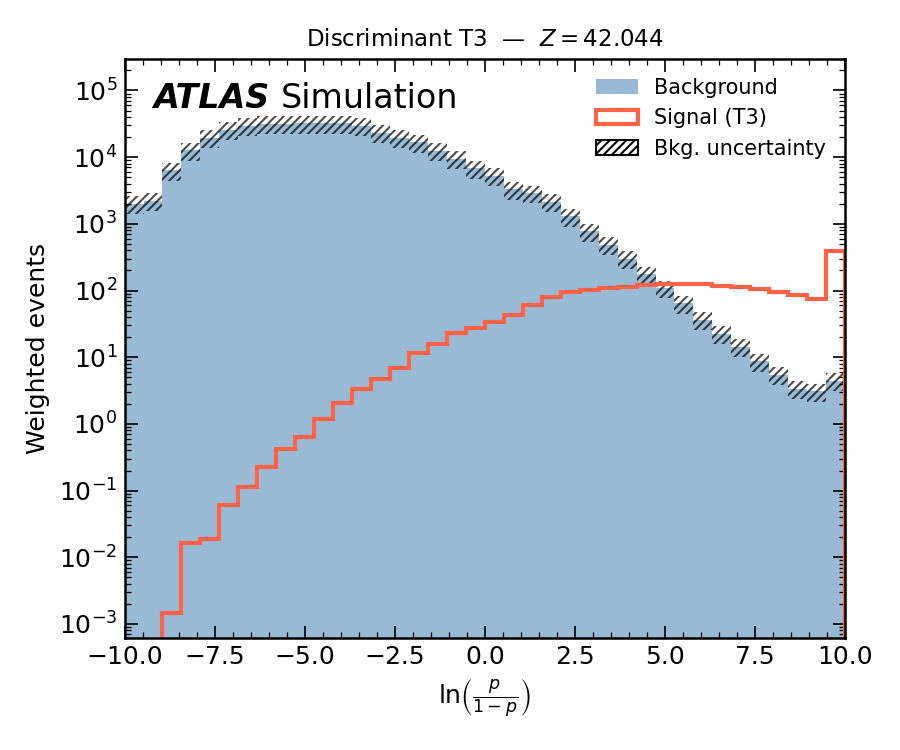
\includegraphics[width=\textwidth]{significance_plots-vbfrnn-v3-equal-signal-crosssection/binary_groups/binary_discriminants_allS_allM_allT_T3.png}\caption{$T_3$.}\end{subfigure}

\medskip

\begin{subfigure}[b]{0.32\textwidth}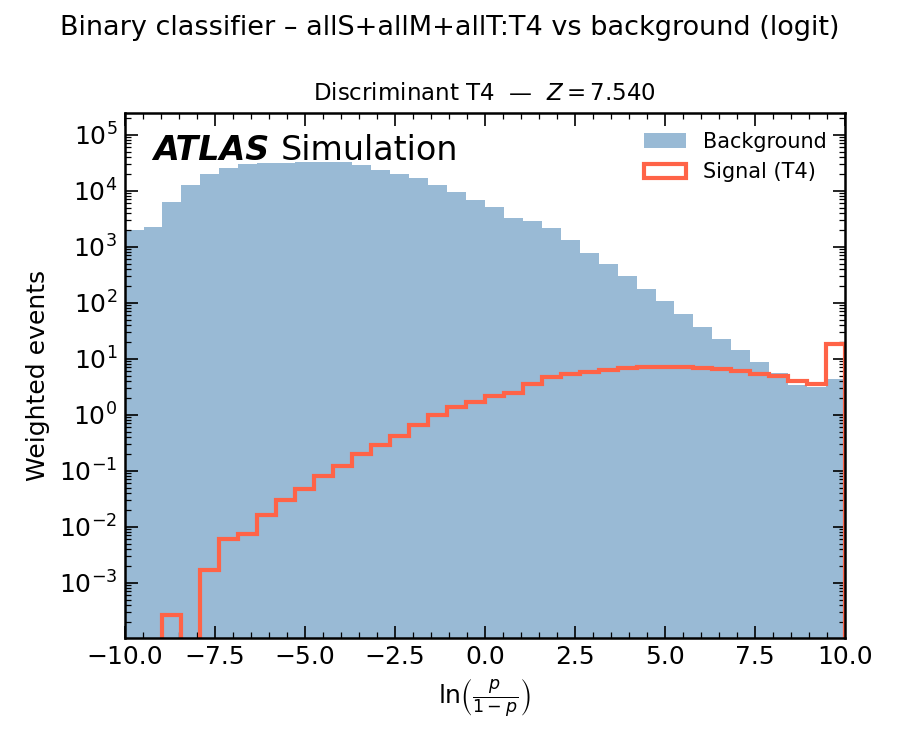
\includegraphics[width=\textwidth]{significance_plots-vbfrnn-v3-equal-signal-crosssection/binary_groups/binary_discriminants_allS_allM_allT_T4.png}\caption{$T_4$.}\end{subfigure}\hfill
\begin{subfigure}[b]{0.32\textwidth}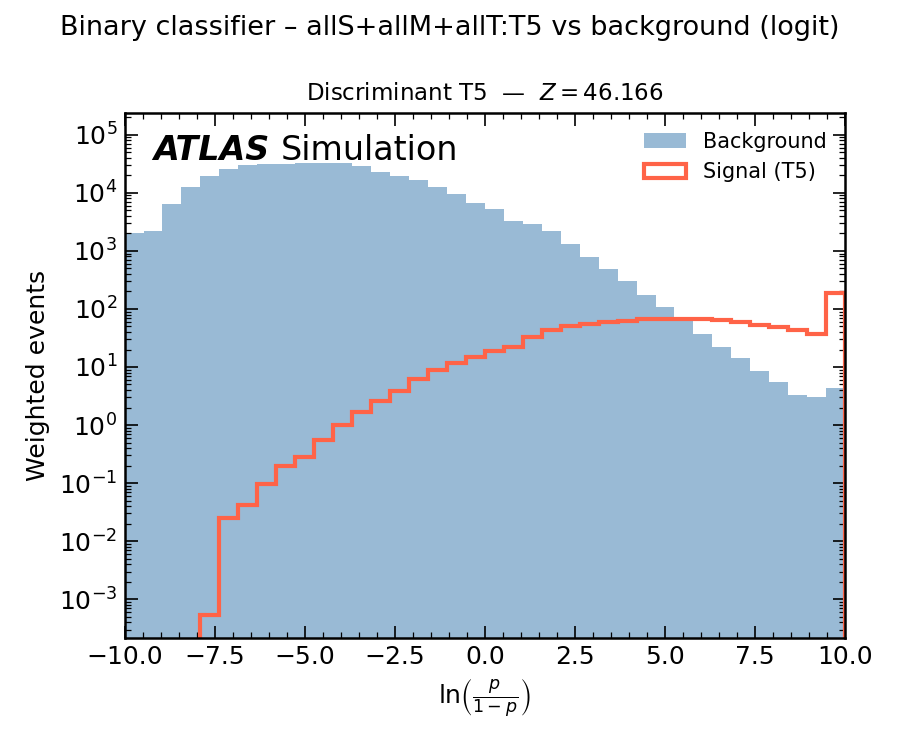
\includegraphics[width=\textwidth]{significance_plots-vbfrnn-v3-equal-signal-crosssection/binary_groups/binary_discriminants_allS_allM_allT_T5.png}\caption{$T_5$.}\end{subfigure}\hfill
\begin{subfigure}[b]{0.32\textwidth}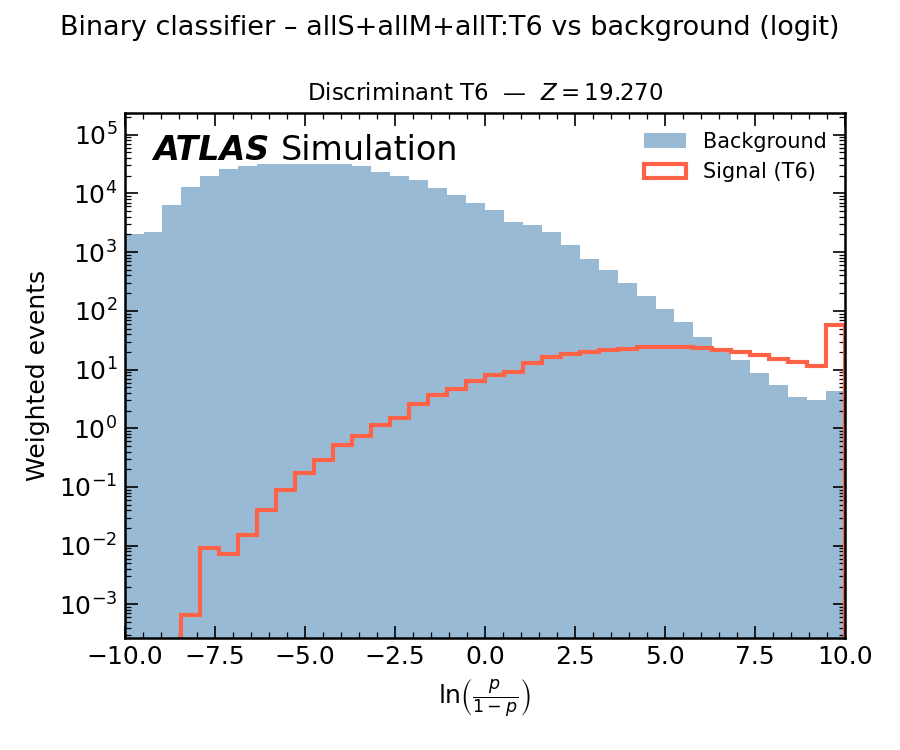
\includegraphics[width=\textwidth]{significance_plots-vbfrnn-v3-equal-signal-crosssection/binary_groups/binary_discriminants_allS_allM_allT_T6.png}\caption{$T_6$.}\end{subfigure}

\medskip

\begin{subfigure}[b]{0.32\textwidth}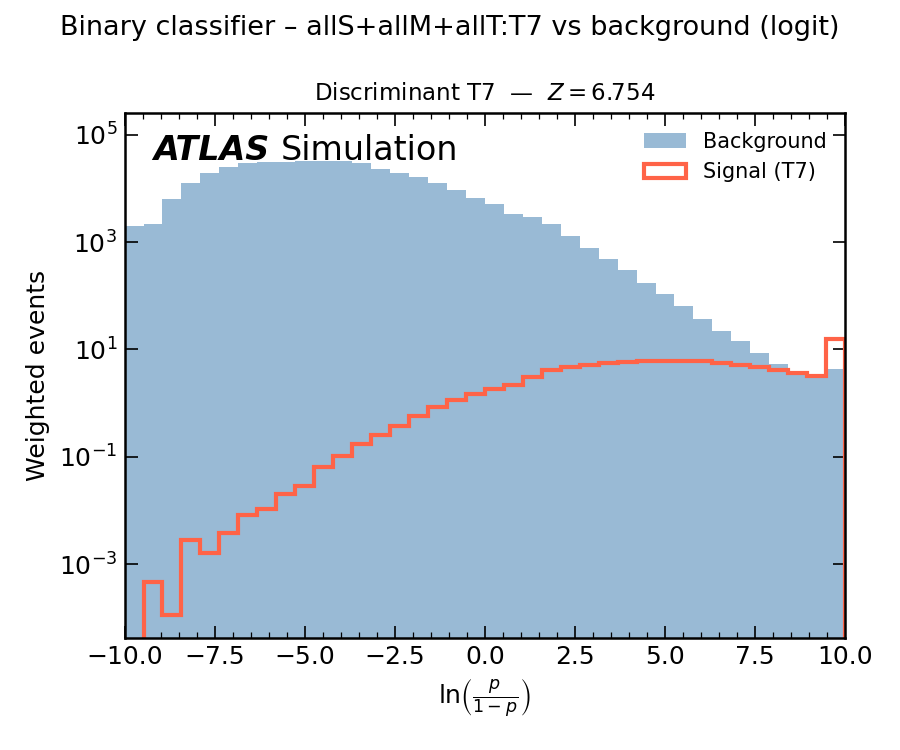
\includegraphics[width=\textwidth]{significance_plots-vbfrnn-v3-equal-signal-crosssection/binary_groups/binary_discriminants_allS_allM_allT_T7.png}\caption{$T_7$.}\end{subfigure}\hfill
\begin{subfigure}[b]{0.32\textwidth}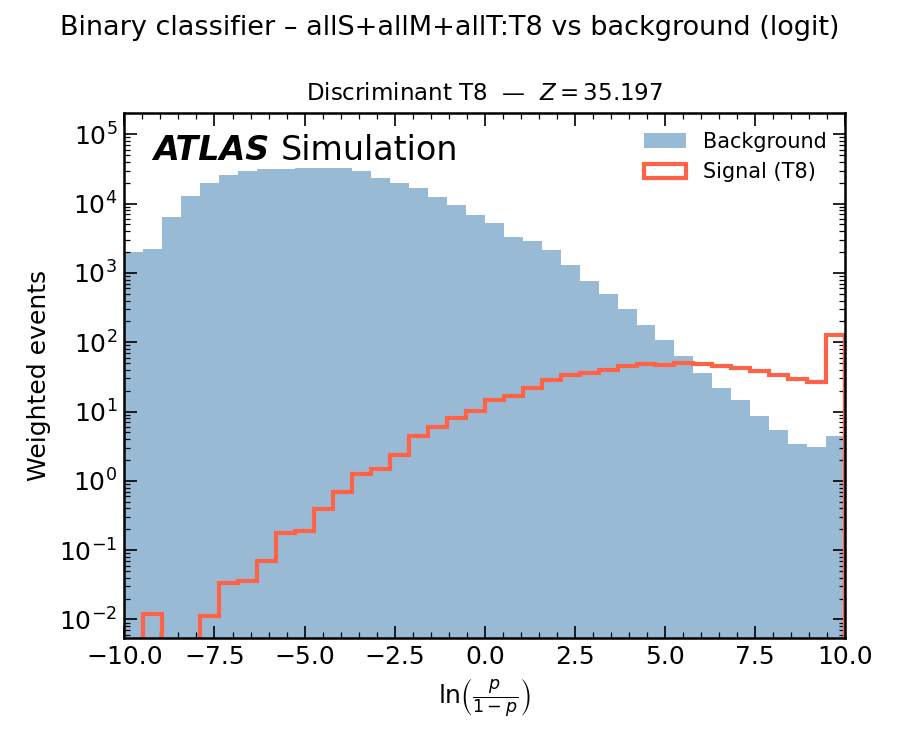
\includegraphics[width=\textwidth]{significance_plots-vbfrnn-v3-equal-signal-crosssection/binary_groups/binary_discriminants_allS_allM_allT_T8.png}\caption{$T_8$.}\end{subfigure}\hfill
\begin{subfigure}[b]{0.32\textwidth}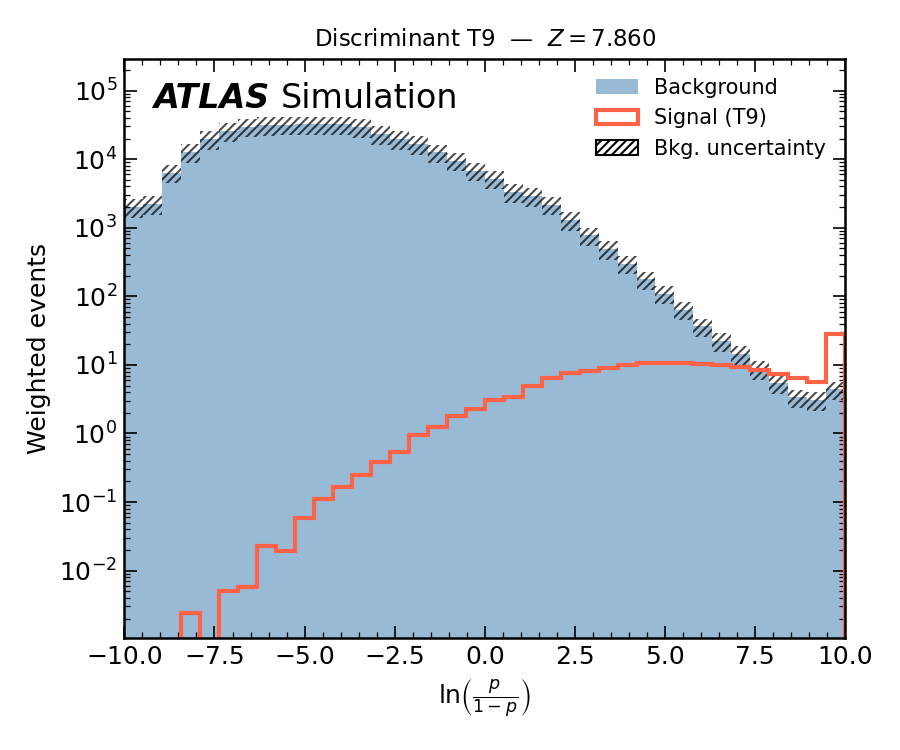
\includegraphics[width=\textwidth]{significance_plots-vbfrnn-v3-equal-signal-crosssection/binary_groups/binary_discriminants_allS_allM_allT_T9.png}\caption{$T_9$.}\end{subfigure}
\caption{Global binary discriminant on the v3~+~equal-$\sigma$ configuration for the tensor operators.}
\label{fig:app_disc_v3eq_global_T}
\end{figure}

\begin{figure}[htbp]
\centering
\begin{subfigure}[b]{0.32\textwidth}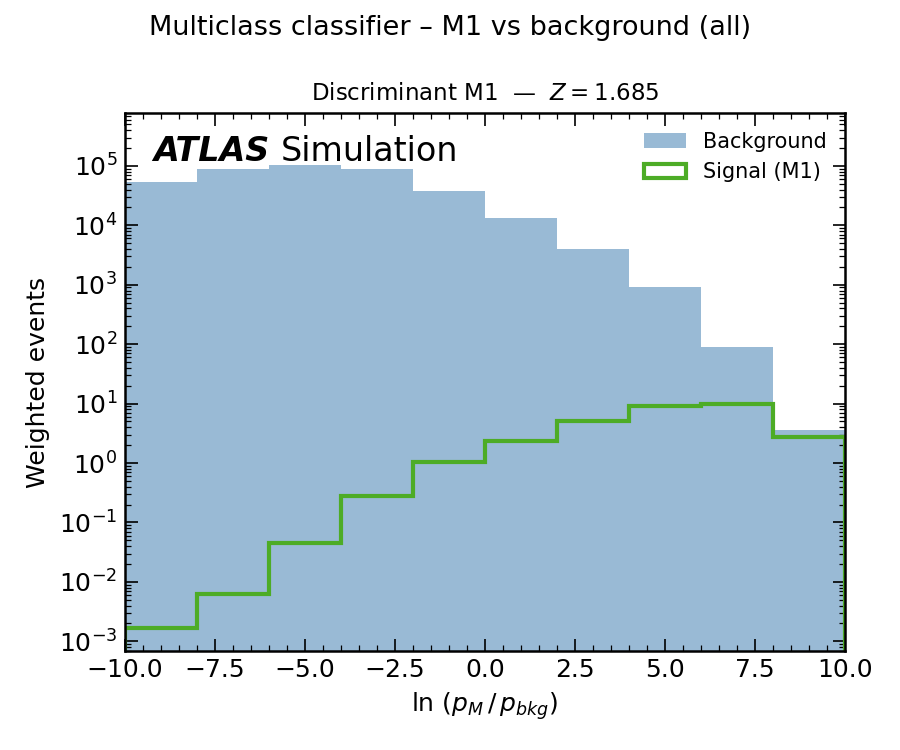
\includegraphics[width=\textwidth]{significance_plots-vbfrnn-v3-equal-signal-crosssection/multiclass/multiclass_discriminants_all_M1.png}\caption{$M_1$.}\end{subfigure}\hfill
\begin{subfigure}[b]{0.32\textwidth}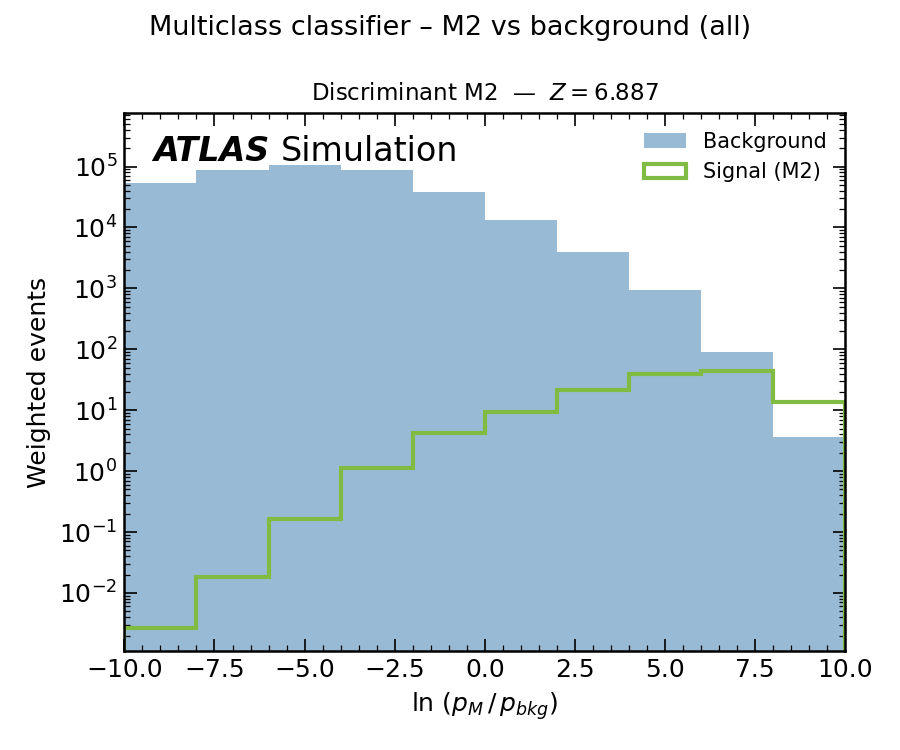
\includegraphics[width=\textwidth]{significance_plots-vbfrnn-v3-equal-signal-crosssection/multiclass/multiclass_discriminants_all_M2.png}\caption{$M_2$.}\end{subfigure}\hfill
\begin{subfigure}[b]{0.32\textwidth}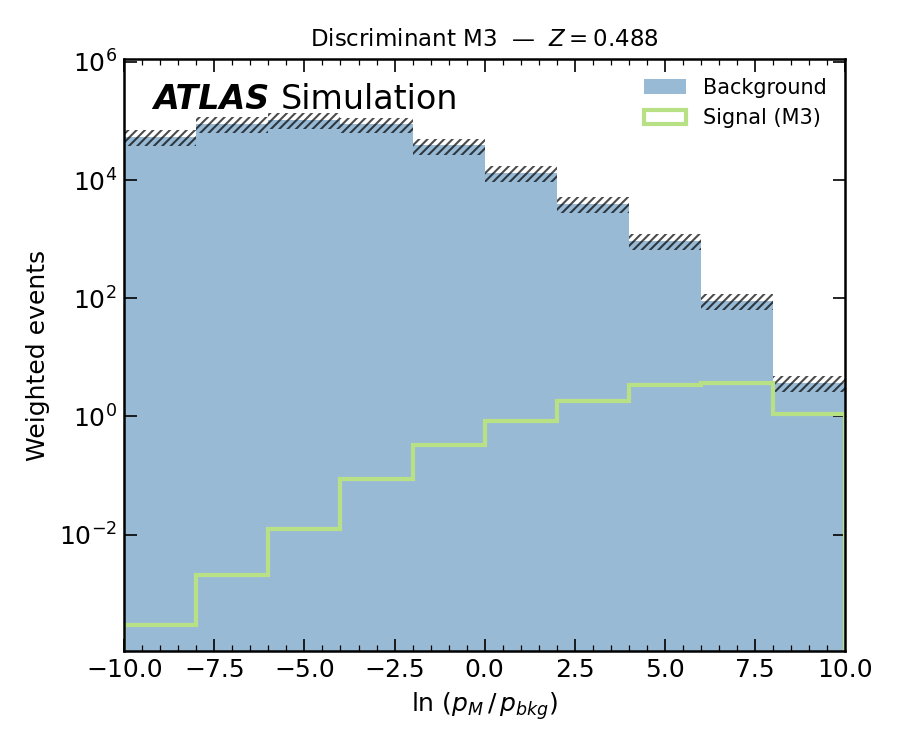
\includegraphics[width=\textwidth]{significance_plots-vbfrnn-v3-equal-signal-crosssection/multiclass/multiclass_discriminants_all_M3.png}\caption{$M_3$.}\end{subfigure}

\medskip

\begin{subfigure}[b]{0.32\textwidth}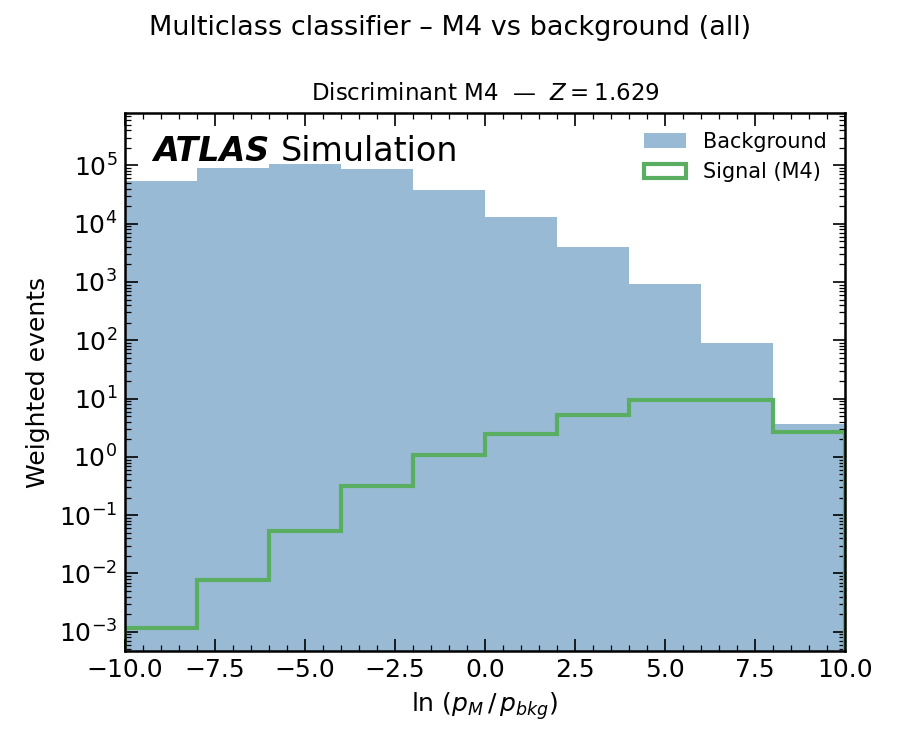
\includegraphics[width=\textwidth]{significance_plots-vbfrnn-v3-equal-signal-crosssection/multiclass/multiclass_discriminants_all_M4.png}\caption{$M_4$.}\end{subfigure}\hfill
\begin{subfigure}[b]{0.32\textwidth}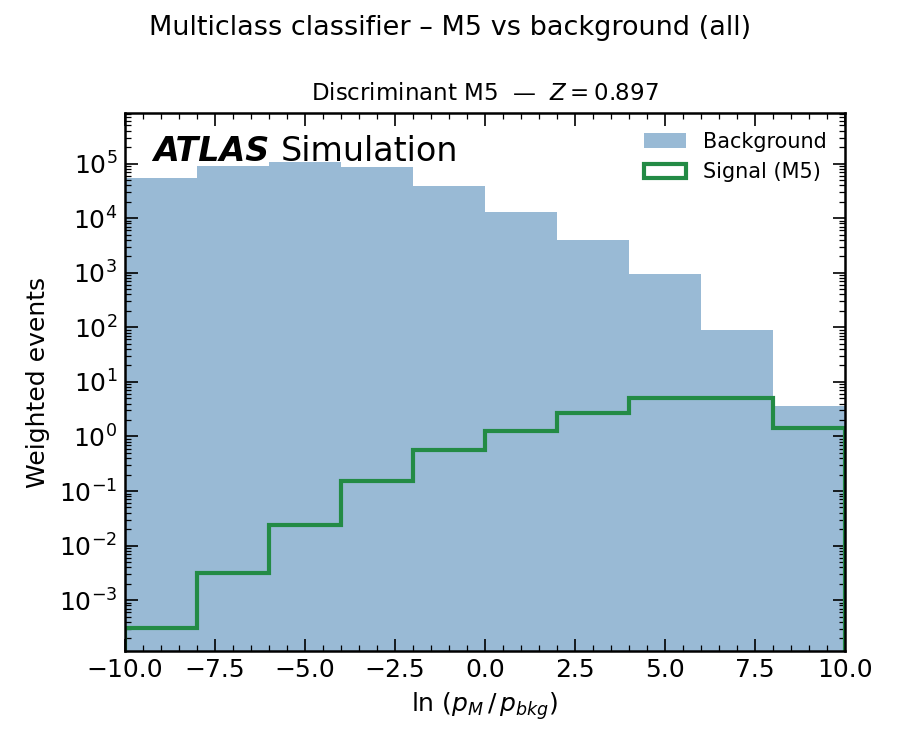
\includegraphics[width=\textwidth]{significance_plots-vbfrnn-v3-equal-signal-crosssection/multiclass/multiclass_discriminants_all_M5.png}\caption{$M_5$.}\end{subfigure}\hfill
\begin{subfigure}[b]{0.32\textwidth}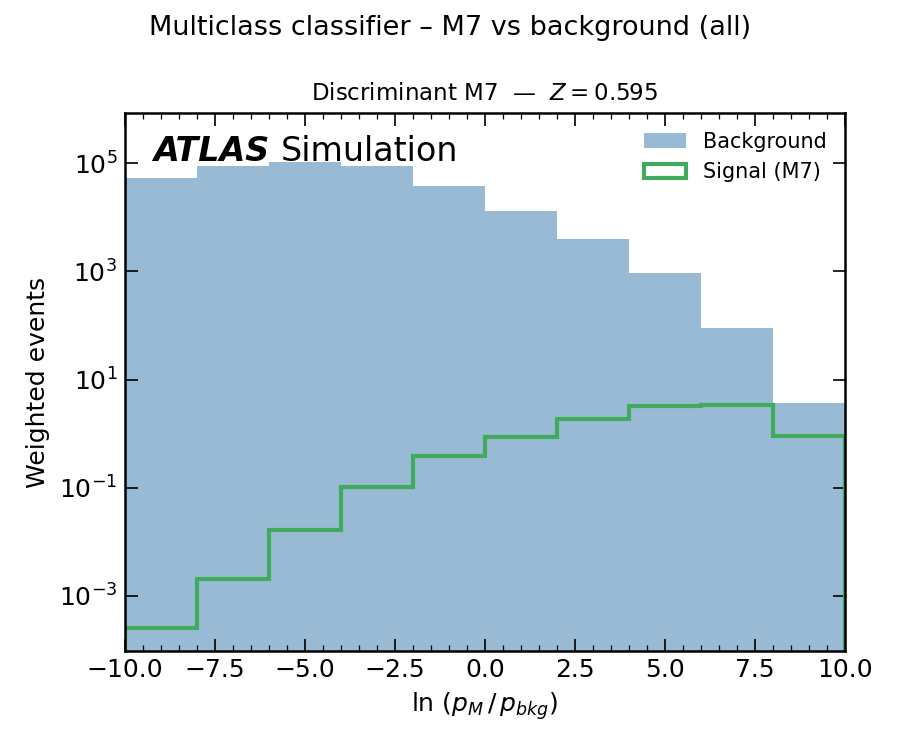
\includegraphics[width=\textwidth]{significance_plots-vbfrnn-v3-equal-signal-crosssection/multiclass/multiclass_discriminants_all_M7.png}\caption{$M_7$.}\end{subfigure}
\caption{Multi-class discriminant on the v3~+~equal-$\sigma$ configuration for the mixed operators.}
\label{fig:app_disc_v3eq_mc_M}
\end{figure}

\begin{figure}[htbp]
\centering
\begin{subfigure}[b]{0.32\textwidth}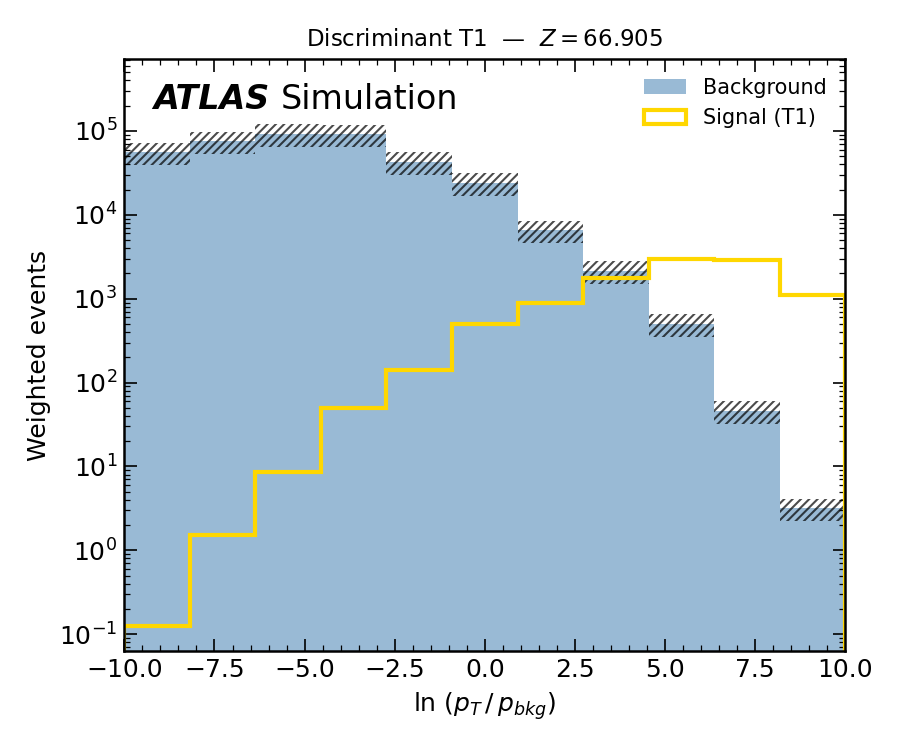
\includegraphics[width=\textwidth]{significance_plots-vbfrnn-v3-equal-signal-crosssection/multiclass/multiclass_discriminants_all_T1.png}\caption{$T_1$.}\end{subfigure}\hfill
\begin{subfigure}[b]{0.32\textwidth}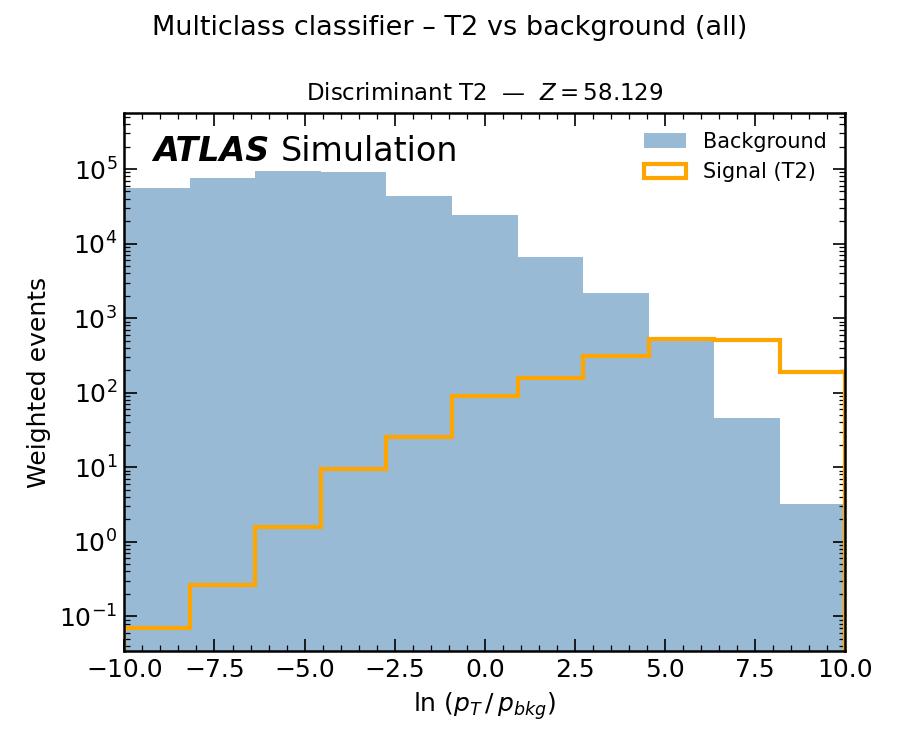
\includegraphics[width=\textwidth]{significance_plots-vbfrnn-v3-equal-signal-crosssection/multiclass/multiclass_discriminants_all_T2.png}\caption{$T_2$.}\end{subfigure}\hfill
\begin{subfigure}[b]{0.32\textwidth}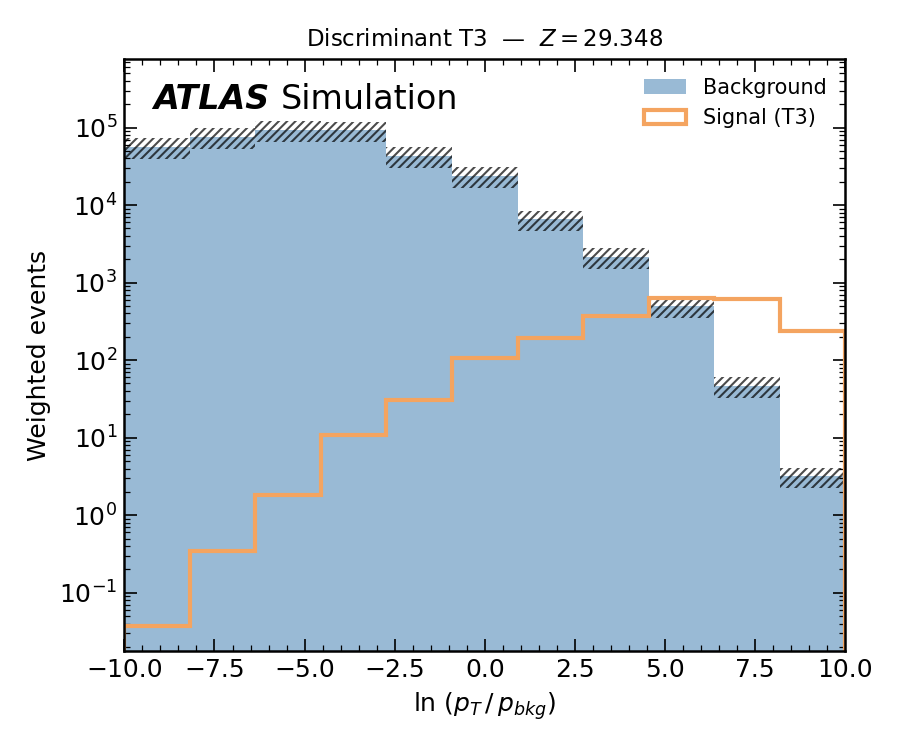
\includegraphics[width=\textwidth]{significance_plots-vbfrnn-v3-equal-signal-crosssection/multiclass/multiclass_discriminants_all_T3.png}\caption{$T_3$.}\end{subfigure}

\medskip

\begin{subfigure}[b]{0.32\textwidth}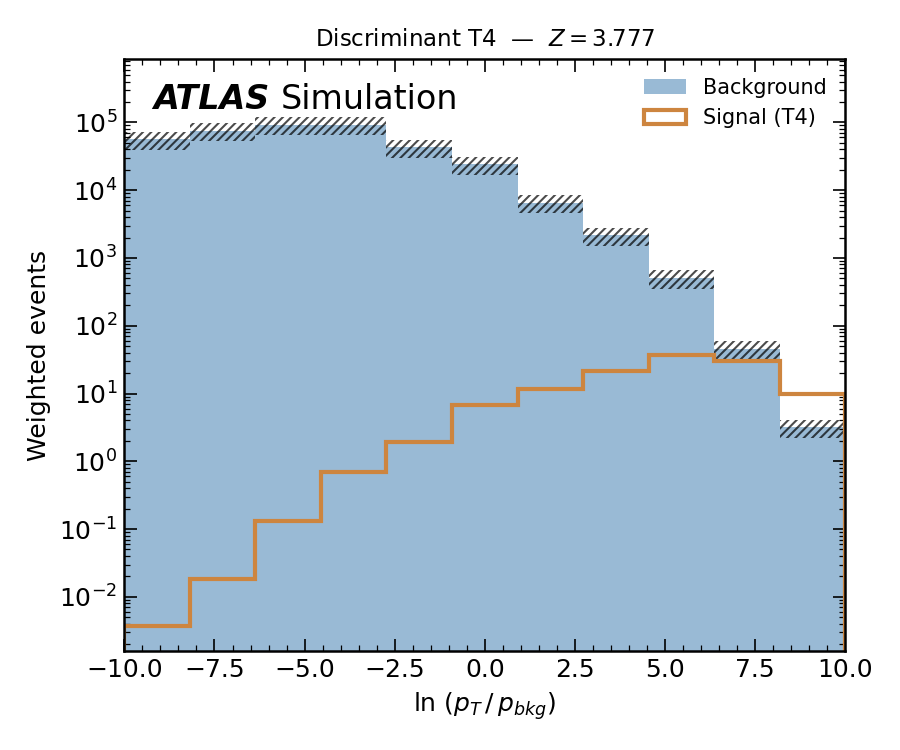
\includegraphics[width=\textwidth]{significance_plots-vbfrnn-v3-equal-signal-crosssection/multiclass/multiclass_discriminants_all_T4.png}\caption{$T_4$.}\end{subfigure}\hfill
\begin{subfigure}[b]{0.32\textwidth}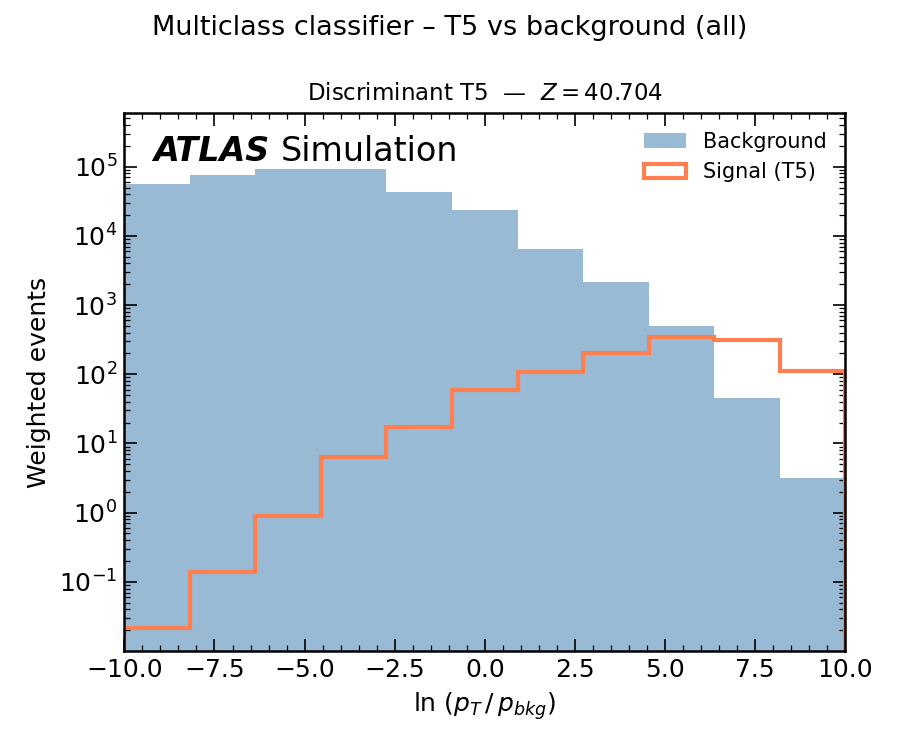
\includegraphics[width=\textwidth]{significance_plots-vbfrnn-v3-equal-signal-crosssection/multiclass/multiclass_discriminants_all_T5.png}\caption{$T_5$.}\end{subfigure}\hfill
\begin{subfigure}[b]{0.32\textwidth}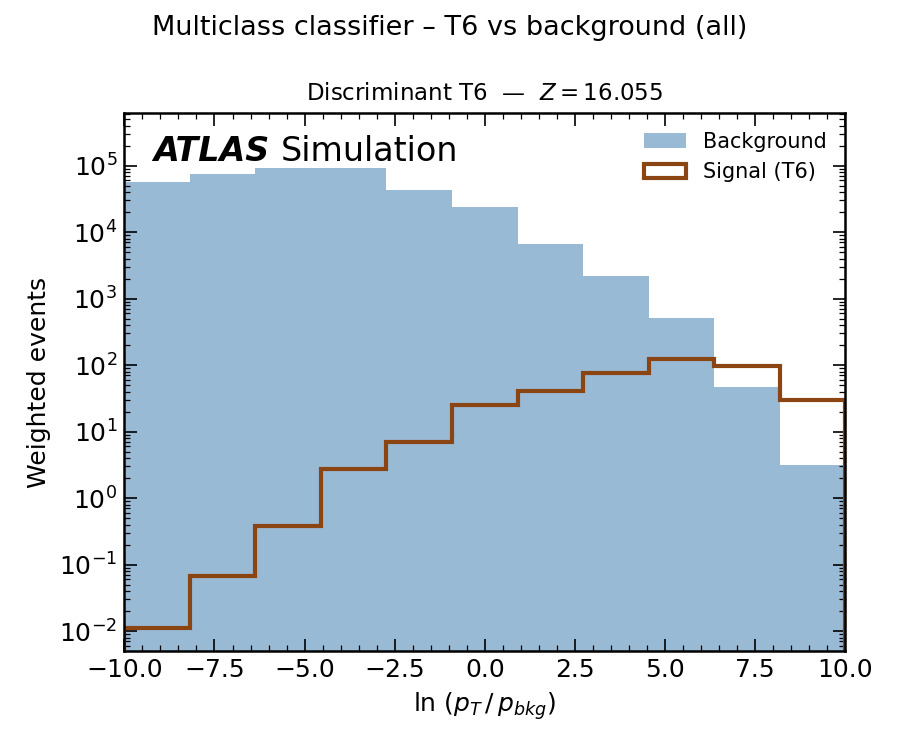
\includegraphics[width=\textwidth]{significance_plots-vbfrnn-v3-equal-signal-crosssection/multiclass/multiclass_discriminants_all_T6.png}\caption{$T_6$.}\end{subfigure}

\medskip

\begin{subfigure}[b]{0.32\textwidth}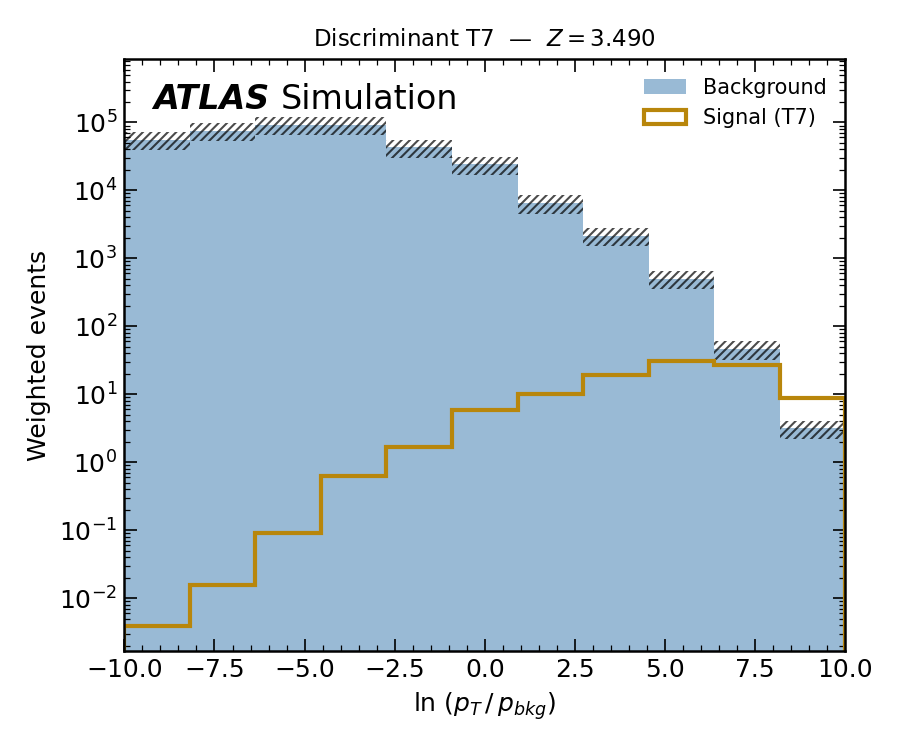
\includegraphics[width=\textwidth]{significance_plots-vbfrnn-v3-equal-signal-crosssection/multiclass/multiclass_discriminants_all_T7.png}\caption{$T_7$.}\end{subfigure}\hfill
\begin{subfigure}[b]{0.32\textwidth}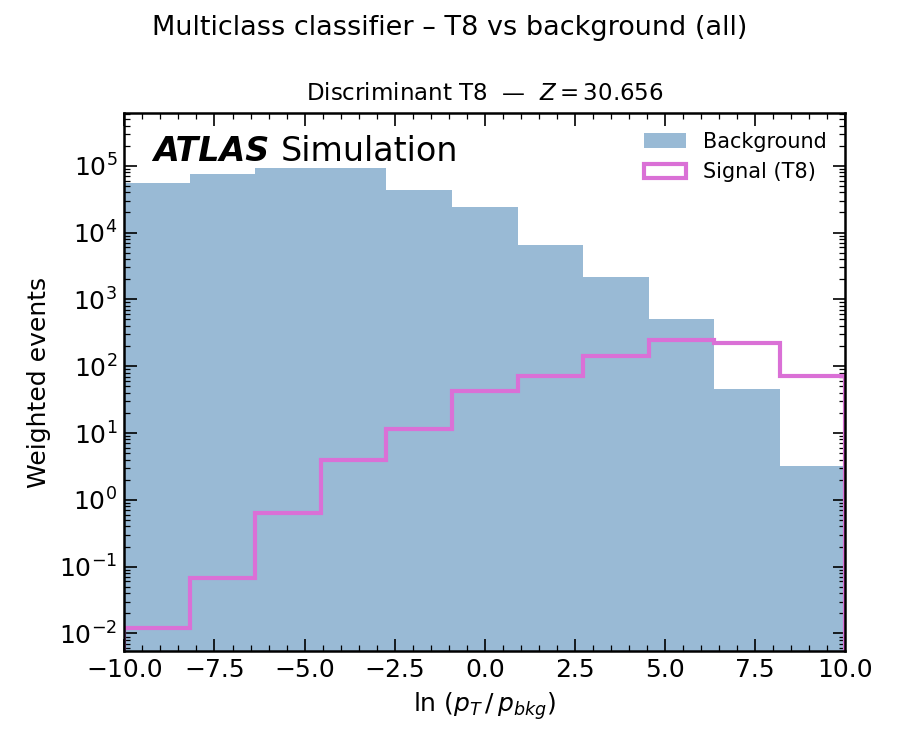
\includegraphics[width=\textwidth]{significance_plots-vbfrnn-v3-equal-signal-crosssection/multiclass/multiclass_discriminants_all_T8.png}\caption{$T_8$.}\end{subfigure}\hfill
\begin{subfigure}[b]{0.32\textwidth}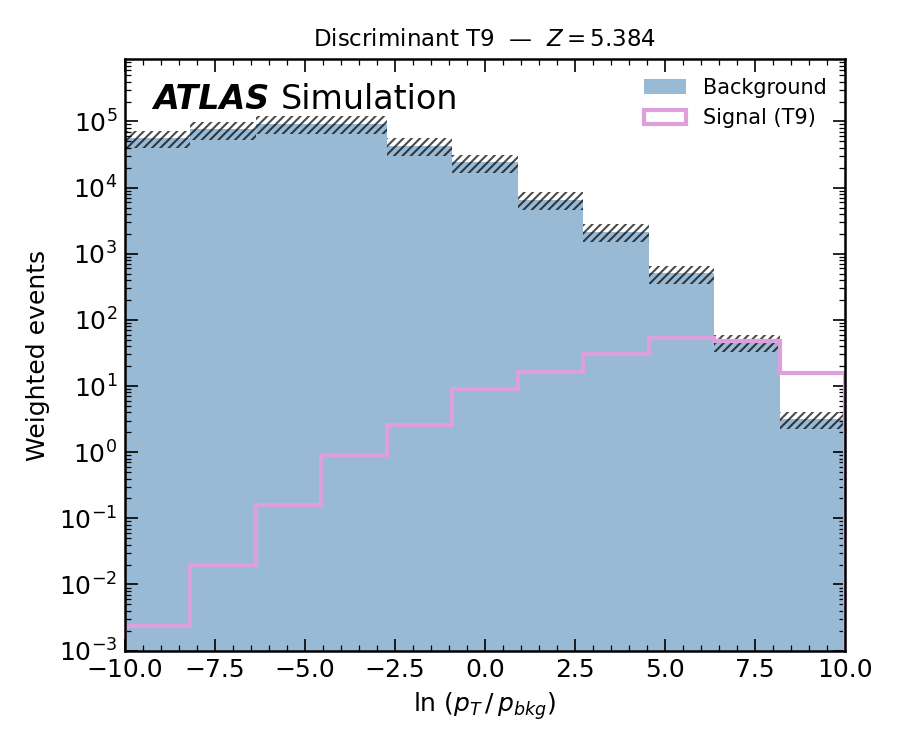
\includegraphics[width=\textwidth]{significance_plots-vbfrnn-v3-equal-signal-crosssection/multiclass/multiclass_discriminants_all_T9.png}\caption{$T_9$.}\end{subfigure}
\caption{Multi-class discriminant on the v3~+~equal-$\sigma$ configuration for the tensor operators.}
\label{fig:app_disc_v3eq_mc_T}
\end{figure}
